% User guide for the cronologic GmbH & Co. KG TimeTagger4 and xTDC4 boards.
%
% to create user guides with the correct filenames run the parent configuration files like this
% pdflatex xTDC4_User_Guide.tex
% pdflatex TimeTagger4_User_Guide.tex
% 
% Visit www.cronologic.de for ready made PDFs of these user guides
% https://www.cronologic.de/products/tdcs/xtdc4-pcie 
% https://www.cronologic.de/products/tdcs/timetagger
%
% You can contribute to this documentation at
% https://github.com/cronologic-de/ug_xtdc4_timetagger
%
% the whole user guide is provided by cronologic GmbH & Co. KG under a
% Creative Commons Attribution-NoDerivatices 4.0 International License
% https://creativecommons.org/licenses/by-nd/4.0/
% except fpr extraplaceins.sty which is in the public domain

% configure Visual Studio Code LaTeX Workshop 
% !TEX root = xHPTDC8_User_guide.tex
  
\documentclass[11pt,notitlepage]{scrreprt}
\usepackage{cronologicug}

% this file creates two similar user guides depending on the commend \deviceName
 
%source files that differ between versions can be input with \ttinput
%this will prefix the include with TT4_ or xTDC4, depending on versoin

\usepackage{ifthen}
% instead of setting \devicename in a top level file you can also provide it at the command line
% pdflatex "\newcommand{\deviceName}{xTDC4} % User guide for the cronologic GmbH & Co. KG TimeTagger4 and xTDC4 boards.
%
% To create user guides with the correct filenames run the parent configuration
% files like this
% lualatex xTDC4_User_Guide.tex
% lualatex TimeTagger4_User_Guide.tex
% lualatex xHPTDC8_User_Guide.tex
% 
% Visit https://docs.cronologic.de for ready made PDFs of these user guides
%
% You can contribute to this documentation at
% https://github.com/cronologic-de/ug_xtdc_timetagger_xhptdc/
%
% the whole user guide is provided by cronologic GmbH & Co. KG under a
% Creative Commons Attribution-NoDerivatices 4.0 International License
% https://creativecommons.org/licenses/by-nd/4.0/
% except fpr extraplaceins.sty which is in the public domain

% configure Visual Studio Code LaTeX Workshop 
% !TEX root = xHPTDC8_User_guide.tex
  
\documentclass[12pt,notitlepage,a4paper]{report}
\usepackage[
    font=montserrat,
    monofontdescriptions,
    pdfkeywords={User Guide, cronologic, TDC, time-to-digital converter,
                 \deviceName}
]{cronologicug}
 
\ifthenelse{\isundefined{\deviceName}}{ 
    \message {\\ WARNING: Undefined device name, TimeTagger4 used}%
    \newcommand{\deviceName}{TimeTagger4}%
    \newcommand{\adeviceName}{a TimeTagger4}%
    }{}
\message{\\Device name is \deviceName }

\title{\deviceName{} -- User Guide, Rev. \ugrev}

% output the first option for the TimeTagger, the second one otherwise
% example: 
% \itett{THIS IS A TimeTagger4}{THIS IS NOT}
\ifthenelse{\equal{\deviceName}{TimeTagger4}}{
    \newcommand{\itett}[2]{#1}
}{
    \newcommand{\itett}[2]{#2}
}
\itett{\message{\\TIMETAGGER\\}}{\message{\\NO TIMETAGGER\\}}

% output code only for the xHPTDC8 
% example: 
% \ifXHPTDC{THIS IS AN xHPTDC8}{THIS IS NOT}
% NOTE: Macro names may not contain digits
\ifthenelse{\equal{\deviceName}{xHPTDC8}}{
    \newcommand{\ifxHPTDC}[2]{#1}
}{
    \newcommand{\ifxHPTDC}[2]{#2}
}
\ifxHPTDC{\message{\\XHPTDC8\\}}{\message{\\NO XHPTDC8\\}}
 
% output code for the TimeTagger4, xTDC4 or xHPTDC8
% example: 
% \txh{THIS IS A TimeTagger4}{THIS IS AN xTDC4}{THIS IS AN xHPTDC8}
\itett{
    \newcommand{\txh}[3]{#1}
}{
    \ifxHPTDC{
        \newcommand{\txh}[3]{#3}
    }{
        \newcommand{\txh}[3]{#2}
    }
}

% set default values in API's description lists
\newcommand{\txhinits}[3]{\normalfont\ttfamily\txh{#1}{#2}{\ =\ #3;}}
 
\txh{ % TimeTagger4
    \message{Generating User Guide for TimeTagger4}
    \newcommand{\ttinput}[1]{\input{timetagger/#1}}
    \newcommand{\titlefile}{"figures/TT4_title.pdf"}
    \newcommand{\prefix}{timetagger4\tu}
    \newcommand{\PREFIX}{TIMETAGGER4\tu}
}{ % xTDC4
    \message{Generating User Guide for xTDC4}
    \newcommand{\ttinput}[1]{\input{xtdc/#1}}
    \newcommand{\titlefile}{"figures/xTDC4_title.pdf"}
    \newcommand{\prefix}{xtdc4\tu} 
    \newcommand{\PREFIX}{XTDC4\tu}
} 
{ % xHPTDC8
    \message{Generating User Guide for xHPTDC8}
    \newcommand{\ttinput}[1]{\input{xhptdc/#1}}
    \newcommand{\titlefile}{figures/xHPTDC8_title.pdf}
    \newcommand{\prefix}{xhptdc8\tu}
    \newcommand{\PREFIX}{XHPTDC8\tu}
} 

\ifxHPTDC{
    \newcommand{\longlong}{int64\tu t} 
    \newcommand{\uint}{uint32\tu t}
    \newcommand{\ushort}{uint16\tu t}
    \newcommand{\uchar}{uint8\tu t}	
}{
    \newcommand{\longlong}{\tu \tu int64}
    \newcommand{\uint}{unsigned int}
    \newcommand{\ushort}{unsigned short}
    \newcommand{\uchar}{unsigned char}	
}


\hyphenation{Time-Tagger xTDC xHPTDC cronologic TimeTagger time-stamps time-stamp}


\newcommand{\ttvar}[2]{\noindent\texttt{\textbf{\textcolor{cronogrey}{#1} \prefix #2}}}%for variable declaration
\newcommand{\ttdef}[1]{\noindent\texttt{\textcolor{cronogrey}{\mbox{\#{}define}} \PREFIX #1}}%for definitions

\newcommand{\ugrev}{{1.8.16-rc}}

%%%%%%%%%%%%%%%%%%%%%%%%%%%%%%%%% 
\begin{document}
\RaggedRight
\sloppy % much fewer overhanging lines
        % may create ugly block text (which we're not using)
\includepdf[pages={-}]{\titlefile} % include title page
\clearpage
\tableofcontents
\clearpage

% 
    \chapter{Introduction}
        \ttinput{Intro.tex}

    \chapter{Hardware}  
        \label{sec:installation-of-board}

\ifxHPTDC{}{
    The \deviceName\ is available as a PCIe plugin board (variant ``-PCIe'', see \hyperlink{cp:ordering_information}{Ordering Information}) or as a desktop solution (variant ``-TBT'').
    %The two variants are shown in Figure~\ref{fig:boards-overview}.
    For a detailed overview of the hardware of the TBT-variant, please refer to our respective \href{https://docs.cronologic.de/projects/tbt2pcie/}{online user guide}.

    % \begin{figure}[htb]
    %     \centering
    %     \itett{
    %         \includegraphics[width=0.9\textwidth]{timetagger/figures/board-overview}
    %     }{

    %         \includegraphics[width=0.9\textwidth]{xtdc/figures/board-overview}
    %     }
    %     \caption{Overview of the PCIe (left) and the TBT (right) variant of the \deviceName.\textcolor{red}{TODO}}
    %     \label{fig:boards-overview}
    % \end{figure}
}

\section{Installing the PCIe Board}
The \deviceName\ board can be installed in any PCIe-CEM slot with x1 or more
lanes.  Make sure that the PC is powered off and that the main power connector is disconnected while installing the board.\par

%
\section{\deviceName\ Inputs and Connectors}
    Figure~\ref{fig:bracket} shows the location of the inputs on the slot
    bracket.  %
    %
    \begin{figure*}[htb]
        \centering
            \ifxHPTDC{
                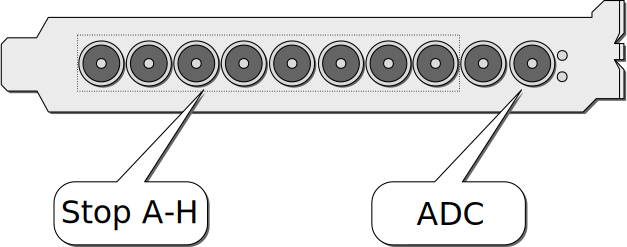
\includegraphics[width=0.6\textwidth]{%
                    figures/xHPTDC8_Slotblende.pdf}
            }{
                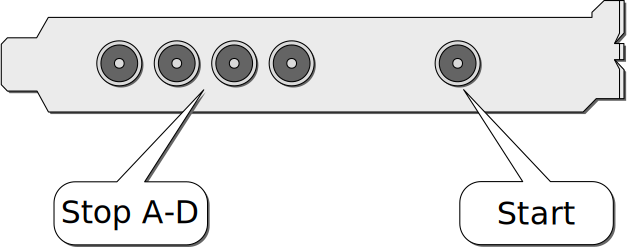
\includegraphics[width=0.6\textwidth]{%
                    figures/xTDC4_Slotblende.pdf}
            }
            \caption{
                Input connectors of the \deviceName\ on the PCIe
                bracket.%
                \ifxHPTDC{
                    Note, the TRG connector acts as a trigger only for the
                    ADC channel, not the TDC channels (see Section~\ref{adc}).
                }{}
                \label{fig:bracket}
            }
    \end{figure*}
    %
    \begin{figure*}[htb]
        \centering
            \ifxHPTDC{
                \includegraphics[width=0.3\textwidth]{%
                    xhptdc/figures/InputCircuit.pdf}
            }{
                \includegraphics[width=0.3\textwidth]{%
                    figures/InputCircuit.pdf}
            }
            \caption{
                Input circuit for each of the input
                channels.
                \ifxHPTDC{
                    Note, the TRG connector acts as a trigger only for the
                    ADC channel, not the TDC channels (see Section~\ref{adc}).
                }{}
                \label{fig:inputcirc}
            }
    \end{figure*}
    %

    LEMO-00 connectors are used for input connection. The inputs are AC-coupled
    and have an impedance of 50\,Ω.  A schematic of the input circuit is shown
    in Figure \ref{fig:inputcirc}.  The digital threshold for any input can be
    adjusted to comply with a multitude of single-ended signaling standards. 
    The threshold can also be used to configure the input for either positive
    or negative pulses.
    
    The connectors can also be used as outputs. 
    \ifxHPTDC{AC-coupled}{DC-coupled} output pulses for automatic internal
    triggering and control of external devices can be generated using the
    TiGer timing pattern generator. See Section~\ref{cp:tiger} for details on
    the TiGer. 
    \ifxHPTDC{
        Furthermore, three inter-board connectors can be found near the top
        edge of the \deviceName\ board, as displayed in
        Figure~\ref{fig:schematics}.  Connector J25 is reserved for future
        use. The pinout of connector J12 is shown in Table~\ref{J12} and the
        pinout of connector J6 is depicted in Table~\ref{J6}.
        Connector J2 is a coax clock input that must receive a 10~MHz clock if
        multiple boards are used together as described in
        Section~\ref{multiboard}.
    }{%TT4 & xTDC4
        Furthermore, for Gen\,1 boards three inter-board connectors can be
        found near the top edge of the \deviceName\ board, as displayed in
        Figure~\ref{fig:schematics}. Connector J25 is reserved for future
        use. The pinout of connector J12 is shown in Table~\ref{J12} and the
        pinout of connector J6 is depicted in Table~\ref{J6}. \textbf{Gen\,2
        boards do not possess these three connectors}.
    }
    %
        \begin{figure*}[htb]
            \centering
                \ifxHPTDC{
                    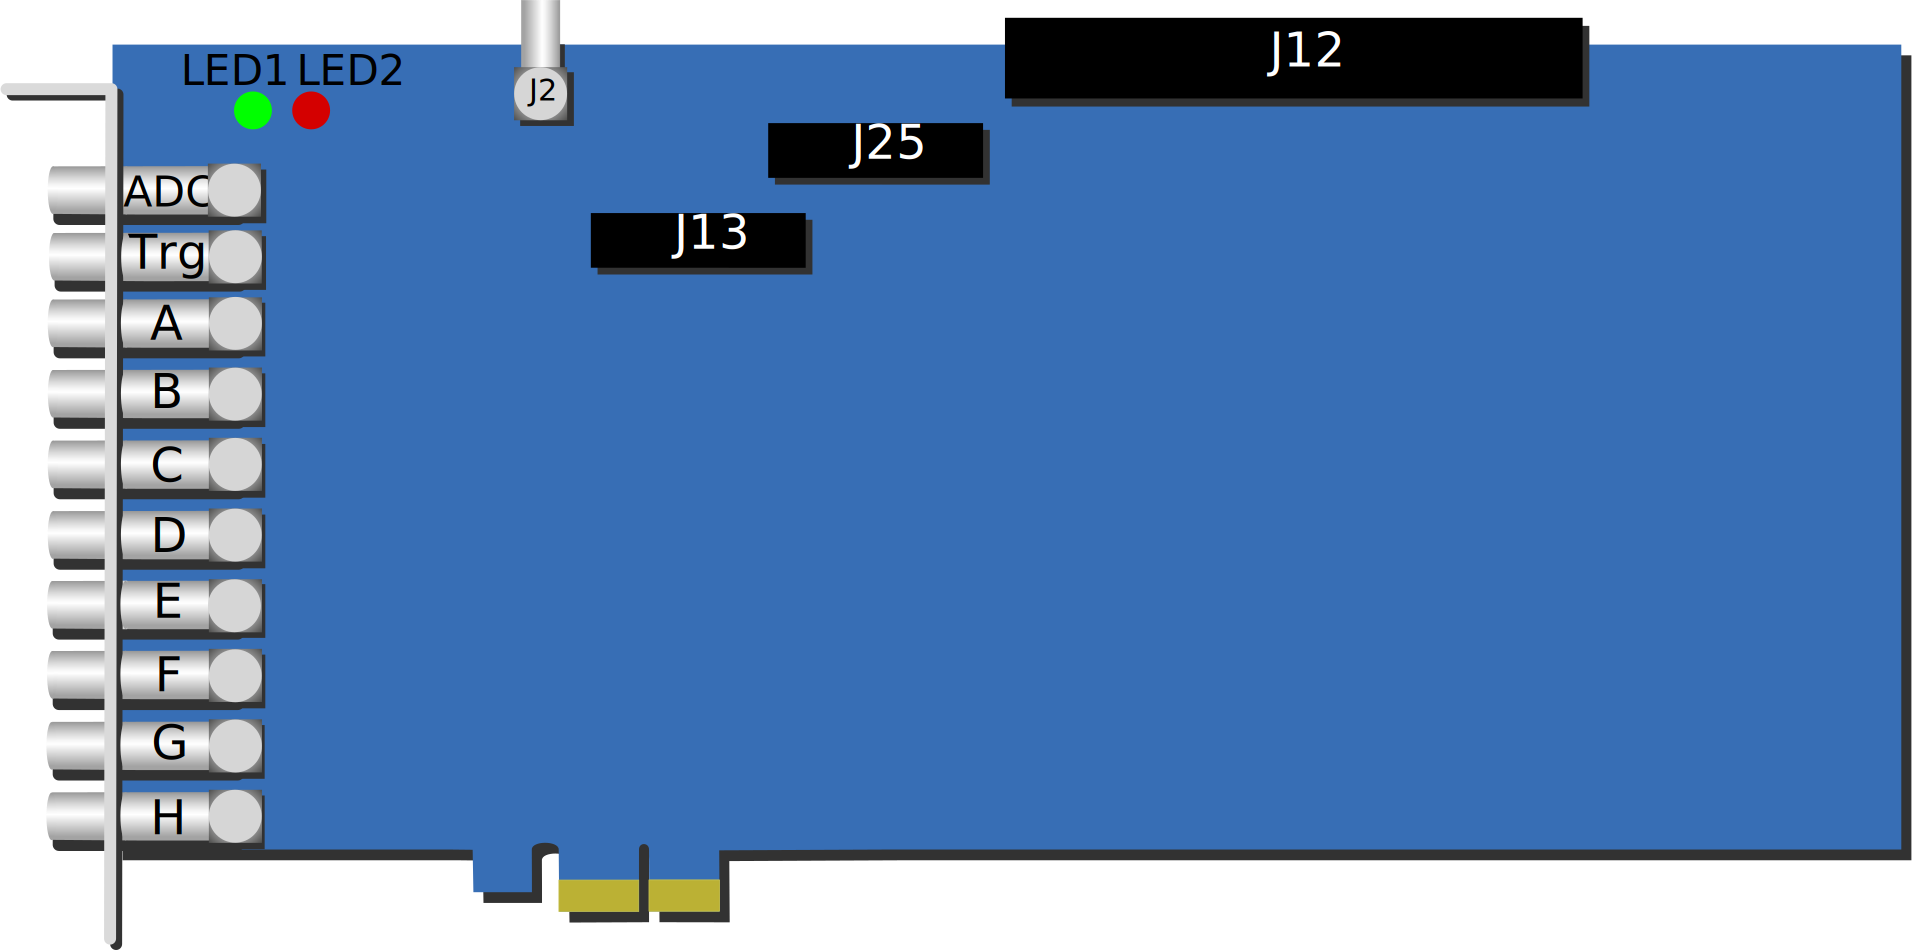
\includegraphics[width=0.7\textwidth]{%
                        xhptdc/figures/xHPTDC8_schematic.pdf}
                }{
                    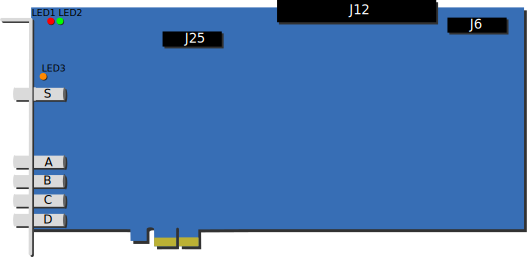
\includegraphics[width=0.7\textwidth]{%
                        figures/xTDC4_schematic.pdf}
                }
                \caption{Schematic view of \adeviceName\ Gen\,1 board showing
                    the inter-board connectors.\label{fig:schematics}}
        \end{figure*}
    %

    \begin{table}
    \begin{small}
        \centering
            \begin{tabular}{|c|c|}
                \hline
                Pin & Name\\
                \hline\hline
                1, 2 & GND\\
                \hline
                3, 4 & external CLK in N, external CLK in P\\
                \hline
                5, 6 & GND\\
                \hline
                7, 8 & reserved/NC\\
                \hline
                9, 10 & GND\\
                \hline
                11, 12 & reserved/NC\\
                \hline
                13, 14 & GND\\
                \hline
                15, 16 & reserved/NC\\
                \hline
                17, 18 & GND\\
                \hline
                19, 20 & reserved/NC\\
                \hline
                21, 22 & GND\\
                \hline
                23, 24 & reserved/NC\\
                \hline
                25, 26 & GND\\
                \hline
                27, 28 & reserved/NC\\
                \hline
                29, 30 & GND\\
                \hline
                31, 32 & reserved/NC\\
                \hline
                33, 34 & GND\\
                \hline
            \end{tabular}
            \caption{Pinout of connector J12.}
            \label{J12}
    \end{small}
    \end{table}

    \begin{table}
    \begin{small}
        \centering
            \begin{tabular}{|c|c|}
                \hline
                Pin & Name\\
                \hline\hline
                1 & +\SI{3.3}{\volt}\\
                \hline
                2 - 9 & reserved/NC\\
                \hline
                10 & GND\\
                \hline
            \end{tabular}
            \caption{Pinout of connector J6.}
            \label{J6}
    \end{small}
    \end{table}

%%%%%%%%%%%%%%% LEDs
\ifxHPTDC{
    \section{Status LEDs}
    Four status LEDs are present on the board. Two are located on the PCB, two more on the PCIe bracket.

    \begin{itemize}
        \item On the PCIe bracket (see Figure~\ref{fig:bracket}): The top LED  lights up green after the board is initialized. The bottom LED lights up briefly while the board is being configured and continuously while the card is capturing.
        \item On the PCB (see Figure~\ref{fig:schematic}): The red LED2 lights up during the configuration of the FPGA and turns off afterward. If it stays permanently lit, the configuration failed. The green LED1 lights up briefly while the board is being configured.
    \end{itemize}
}
{
    \section{Status LEDs of the PCIe boards}
    Three status LEDs are present on the board, as seen in 
    Figure~\ref{fig:schematics}.
    \begin{itemize}
        \item LED1 lights up red during the configuration of the FPGA
            and turns off afterward. If it stays permanently lit, the
            configuration failed.
        \item LED2 lights up green after the board is initialized by the
            driver and turns off when the device is closed by the
            software.
        \item LED3 lights up green when capture is started, yellow after
            the first start signal was detected and red when groups are
            missing.
    \end{itemize}
}

%%%%%%%%%%%%%%% multiboard
\ifxHPTDC{
    \section{Synchronizing multiple boards}
        \label{multiboard}
        If more than eight TDC inputs are required, up to six boards can be
        synchronized within a system. 
        
        The \deviceName\ API described in Chapter~\ref{cp:api} manages up to
        six boards automatically and provides a single data stream that
        contains sorted hit data from all boards in chronological order. 
        Channel A of each board is assigned channel number $\texttt{board\tu
        index} \times 10$.  The \texttt{board\tu index} is assigned to the
        boards in the order of the serial numbers starting at 0.

        \subsection{Connecting multiple boards}
            The boards must each receive a common \SI{10}{\mega\hertz} clock
            signal on connector J2. The connector is inside the PC enclosure. 
            Connectors J12 of all boards must be connected with a flat band
            cable with a terminator at each end.  Cable and Terminator are
            available from cronologic. See Figure~\ref{fig:multiboard} for a
            wiring example.  %
            \begin{figure*}[htb]
                \centering
                    \includegraphics[width=1\textwidth]{
                        xhptdc/figures/multiboard.pdf}				
                    \caption{Synchronizing multiple boards with a
                        ClockBox.\label{fig:multiboard}}
            \end{figure*}
            %
        \subsection{ClockBox}
            For systems of up to four boards, cronologic offers the ClockBox
            product that conveniently makes four clock signals available
            inside the PC enclosure. For use with the \deviceName, jumper JP3
            of the ClockBox must be set as shown in Figure~\ref{fig:clockbox}
            in order to set the clock frequency to \SI{10}{\mega\hertz}. 
            %
            \begin{figure*}[htb]
                \centering
                    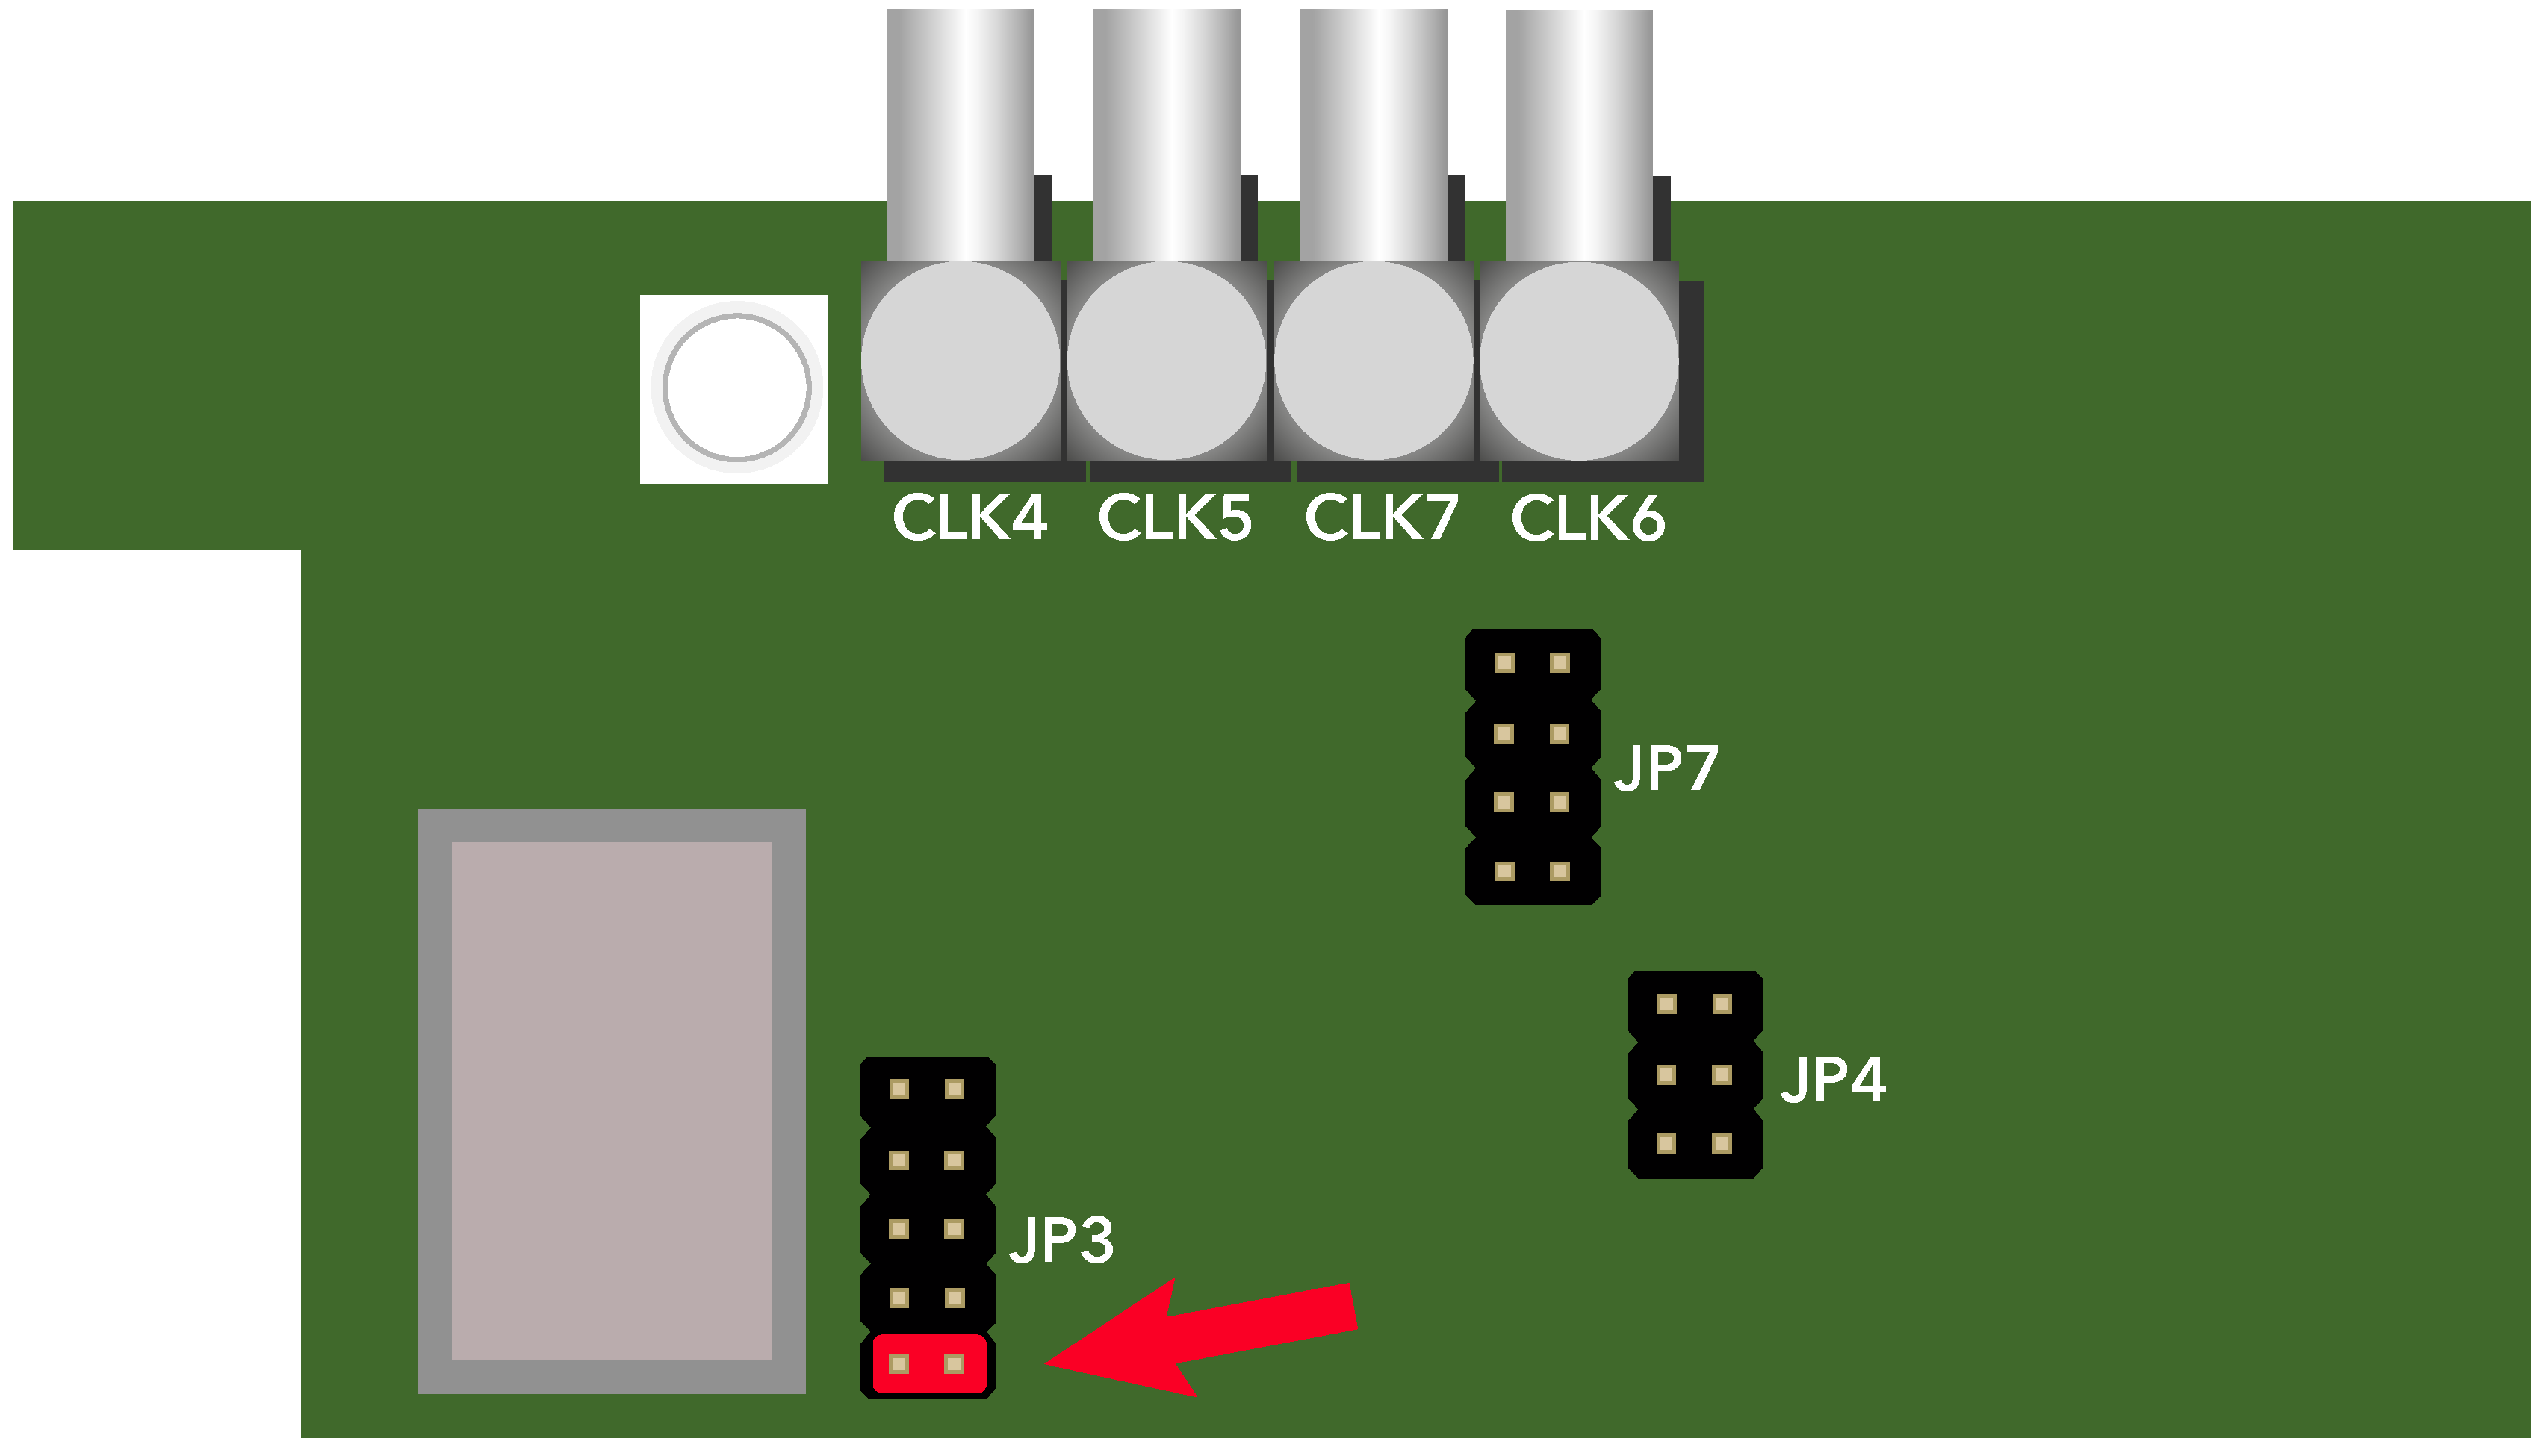
\includegraphics[width=0.5\textwidth]{
                        xhptdc/figures/clockbox.pdf}				
                    \caption{ClockBox jumper setting for
                        \SI{10}{\mega\hertz}.\label{fig:clockbox}}
            \end{figure*}
            %
        
        \subsection{Crates for multiple boards}
            Most PC mainboards don't have enough PCIe slots to support six
            \deviceName s.  We offer an external enclosure called ``Ndigo
            Crate'' that uses PCIe-over-cable technology to extend the number
            of available slots in a system.  The extension is fully
            transparent to the host system. There are no additional drivers
            required.  Please see the
            \href{https://www.cronologic.de/products/pcie/pcie-crates}{%
                product page} at our website \url{www.cronologic.de}.
}{}




    




    \chapter{\deviceName\ Functionality}
        \txh{ %TimeTagger Version
The \deviceName\ is a ``classic'' common start time-to-digital converter. 

It records the time difference between a leading or trailing edge on the start input to the leading and trailing edges of the stop inputs. 
Rising and falling edges of the stop channels A-D can be enabled individually. 
The measurements are quantized as shown in section \ref{sec:features}. 
The timestamps are recorded in integer multiples of the corresponding bin size.
Transitions of the input signals are called hits. To reliably detect hits the signal has to be stable for more than one quantisation interval before and after the edge.  
Triggers on the start channel must not occur less than \SI{5}{\nano\second} apart. The \deviceName\ records events without dead time at a readout rate of about 48\,MHits/s for Gen\,1 and 60\,MHits/s for Gen\,2.
} { %xTDC4 and xHPTDC8 Version
The \deviceName\ is a ``classic'' common start time-to-digital converter. 

It records the time difference between leading or trailing edges on the start input and the stop inputs. 
Each stop channel A-D can be enabled individually. 
The standard deviation of the timestamps is approx. \SI{8}{\pico\second}. 
The timestamps are recorded in integer multiples of a bin size of $5000/(3\cdot 128)$ = $13.0208\overline{3}$\,\si{\pico\second}. 
The data acquisition can be limited to rising or falling signal transitions. 

The maximum trigger rate on the start channel is \SI{4}{\mega\hertz}.

\subsection{Handling of Difficult Hits}
    \label{difficulthits}
    Transitions of the input signals are called hits. To measure all hits with the maximum resolution the hits must fulfill all criteria set forth in this document.
    However, the \deviceName does include mechanisms to provide as much information as possible for hits that fall out of these specs.

    To reliably detect hits the signal has to be stable for at least \SI{900}{\pico\second} before and after the edge that is to be measured. 
    Pulses as short as \SI{250}{\pico\second} are usually detected at full resolution but have a significant chance to be assigned to the wrong group or appear out of order. 
    For these hits bit 7 in the data word is set. See section \ref{flags} for more information on the data format.

    Between multiple hits on a stop channel a dead time of approximately \SI{5}{\nano\second} is required for full resolution. 
    Hits that are closer together will only be reported with a resolution of $5/6$\,\si{\nano\second} = $833\overline{3}$\,\si{\pico\second}. For these hits both bits 6 and 7 are set.

    Data is copied from the 15-entry L0 FIFO to the larger downstream FIFOs at a rate of about \SI{12}{\mega\hertz} per channel. 
    If the L0 FIFO overflows the high resolution measurement of some hits will be discarded. 
    In this case a measurement from an alternative TDC will be used that has a resolution of about \SI{150}{\pico\second}. 
    For these hits bit 6 in the data word will be set
} { %xHPTDC8 version
    The \deviceName\ is a streaming time-to-digital converter. It records the timestamps of changes at the inputs A-H in an infinite stream. 
    A flexible grouping mode is available that can emulate common-start or common-stop behaviour. See section \ref{grouping} for details.

    For each channel, it can be selected individually whether rising or falling edges are recorded. It is not possible to record both edges of the same channel. 
    The timestamps are recorded in integer multiples of a bin size of $5000/(3\cdot 128)$ = $13.0208\overline{3}$\,\si{\pico\second}. 
    There must be at least \SI{5}{\nano\second} between consecutive hits on the same input channel to be detected reliably. 
    The \deviceName\ records events without dead time at a readout rate of about $48$\,MHits/s.
} 
        \section{Grouping and Events}
\label{grouping}
\ifxHPTDC{
    If \textsf{config.tdc\tu mode} is set to \textsf{\PREFIX TDC\tu MODE\tu CONTINOUS} the TDC will operate in grouping mode. 
    This setting only affects data collected using the \textsf{\prefix Read()} method. Data collected using \textsf{\prefix ReadHits()} will always be continous. 
}{} 

In typical applications a start hit is followed by a manifold of hits on e.g. a detector. 
The hits recorded are managed in groups (which are called ``events'' in some applications). 
Figure \ref{fig:grouping} shows a corresponding timing diagram. The user can define the range of a group, i.e. the time window within which hits 
on the stop channels are recorded, in software. Hits occurring outside of that time window are discarded. 
 Different ranges can be set for each of the 4 stop channels by setting corresponding configuration.channel[n].start and .stop values in the channel configuration. 

 \ifxHPTDC{
     The values are configured in picoseconds. Negative values can be used in common stop applications.
     \[ -2^{31} <= start <= stop <= 2^{31}-1 \]
 }{
    The values need to be set as multiples of the bin size and must not be negative.
    \[ 0 <= start <= stop <= 2^{16}-1 \]
 }


%
\begin{figure*}[ht]
    \begin{center}
        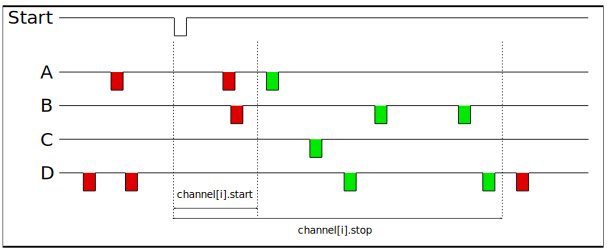
\includegraphics[width=0.7\textwidth]{figures/grouping.pdf}
        \caption{Acquired hits are merged to groups as explained in the text.\label{fig:grouping}}
    \end{center}
\end{figure*}


%
        \lstset{
	language=[Visual]C++,
	keywordstyle=\bfseries\sffamily\color[rgb]{0,0,1},
	identifierstyle=\sffamily,
	commentstyle=\color[rgb]{0.133,0.545,0.133},
	stringstyle=\sffamily\color[rgb]{0.627,0.126,0.941},
	showstringspaces=false,
	basicstyle=\small,
	numberstyle=\footnotesize,
	numbers=left,
	stepnumber=1,
	numbersep=10pt,
	tabsize=2,
	breaklines=true,
	prebreak = \raisebox{0ex}[0ex][0ex]{\ensuremath{\hookleftarrow}},
	breakatwhitespace=false,
	aboveskip={1.5\baselineskip},
	columns=fixed,
	upquote=true,
	extendedchars=true,
}

\section{Auto-Triggering Function Generator\label{cp:AutoTriggeringFunctionGenerator}}
Some applications require internal periodic or random triggering. The \deviceName\ function generator provides this functionality.\par

The delay between two trigger pulses of this trigger generator is the sum of two components: A fixed value M and a pseudo-random value with a range given by the exponent N. \par

The period is

\begin{align}
    T = 1 + M + [1...2^N]
\end{align}

clock cycles \ifxHPTDC{of the 150~MHz clock}{with a duration of $4~ns$ per cycle}.\par

The trigger can be used as a source for the TiGer unit (see Section \ref{cp:tiger}).


\section{Timing Generator (TiGer)\label{cp:tiger}}
Each digital LEMO-00 input can be used as an \ifxHPTDC{AC coupled}{LVCMOS} trigger output. 
The TiGer functionality can be configured independently for each connector. 
See Section \ref{cp:tigerblock} for a full description of the configuration options.
% 
\begin{figure*}[ht]
    \begin{center}
        \ifxHPTDC { 
            % this is an XCIrcuit drawing  convertex from postscript with 
            %ps2pdf.exe -dEPSCrop xhptdc8_trigger_matrix.ps
            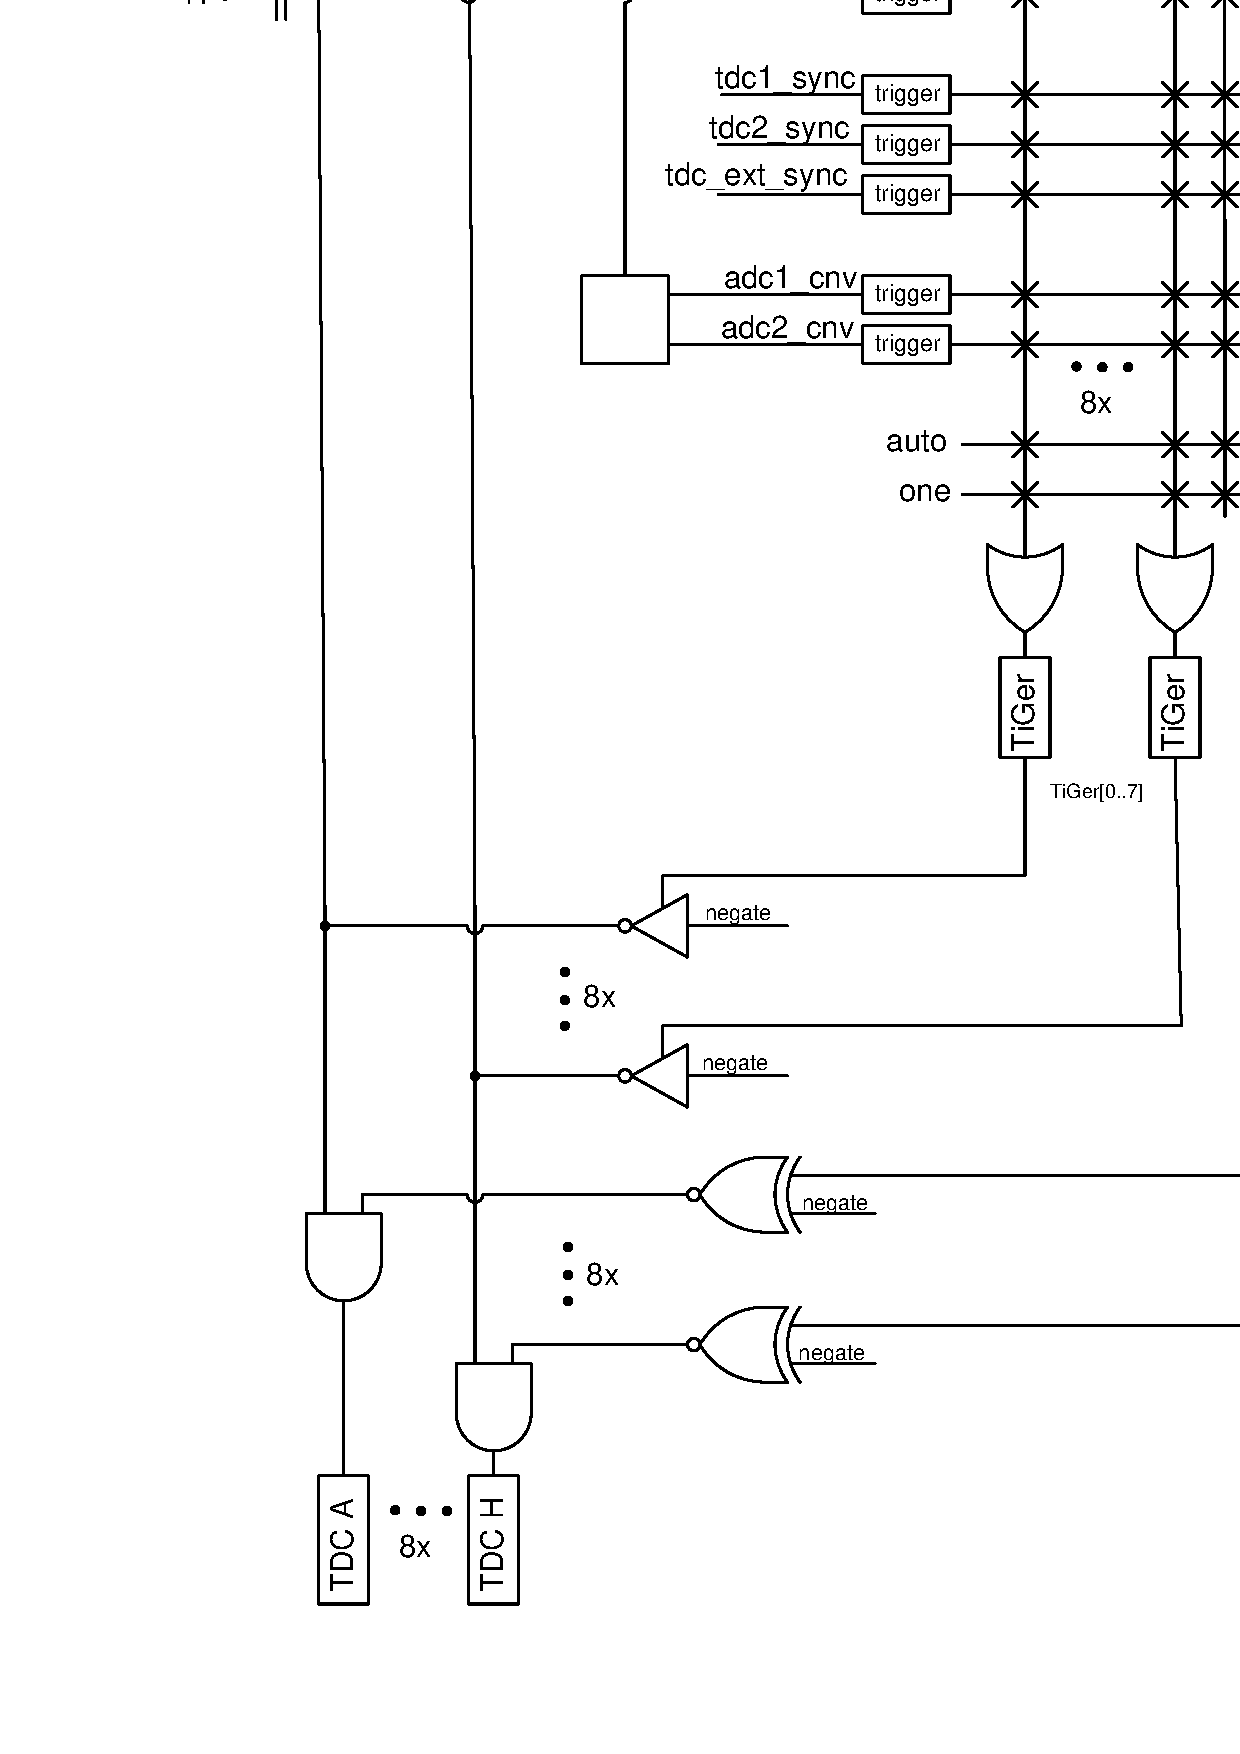
\includegraphics[width=0.6\textwidth]{xhptdc/figures/xhptdc8_trigger_matrix.pdf}
        }{
            \includegraphics[width=0.7\textwidth]{figures/xTDC4_tiger_matrix.pdf}
        }
        \caption{TiGer blocks can generate outputs that are also available on inputs.\label{fig:matrix}} 
    \end{center}
\end{figure*}
%

Figure \ref{fig:matrix} shows how the TiGer blocks are connected. They can be triggered by an OR of an arbitrary combination of inputs, 
including the auto-trigger \ifxHPTDC{and the ADC}{}. Each TiGer can drive its output to its corresponding LEMO connector. This turns the connector into an output. 

\ifxHPTDC{
	The TiGer outputs are AC coupled to the connector. They can be operated in one of the following modes:
	\paragraph*{\textsf{\PREFIX TIGER\tu OFF}} 
		No signal is output to the connetor. 
	\paragraph*{\textsf{\PREFIX TIGER\tu OUTPUT}} 
		In this mode the connector is output only. Pulses are unipolar with 2V amplitude. 
		Connected hardware must not drive any signals to connectors used as outputs, as doing so could damage both the \deviceName\ and the external hardware. 
		We recommend to only use short pulses to avoid undesirable baseline shift due to the AC coupling, but the device does not pose any restrictions on the duty cycle. 
		This mode can be used as a clock output with a frequency of $75/N$~MHz for integer $N$.
	\paragraph*{\textsf{\PREFIX TIGER\tu BIDI}} 
		In this mode the TiGer creates unipolar pulses with 1~V amplitude. The connector can still be used as an input. 
		Use short pulses to keep the probability of collision and the effect on the baseline low.	
	\paragraph*{\textsf{\PREFIX TIGER\tu BIPOLAR}} 
		In this mode the connector creates bipolar pulses with 1~V amplitude. The connector can still be used as an input. 
		Pulses have no effect on the baseline offset. 
		TiGer should be configured with $stop = start$ for minimum width bipolar pulses of $2 \times 6.\overline{6}~ns$. 
		The maximum bipolar pulse width is \textsf{XHPTDC8\tu TIGER\tu MAX\tu BIPOLAR\tu PULSE\tu LENGTH=15}.    
}{
	The TiGer is DC coupled to the connector. Connected hardware must not drive any signals to connectors used as outputs, 
	as doing so could damage both the \deviceName\  and the external hardware.
	Pulses that are short enough for the input AC coupling are available as input signals to the \deviceName. 
	This can be used to measure exact time differences between the generated output signals and input signals on other channels.
}

\ifxHPTDC{
	\newpage
	\subsection{Trigger Sources}
	\label{triggersources}
	Trigger sources for TiGer and gating blocks are configured by a bitmask. You can combine any number of trigger source with a bitwise or. 
	The block will be trigger when any of the select trigger input is active.

	\paragraph*{\textsf{\PREFIX TRIGGER\tu SOURCE\tu NONE}} \leavevmode \\
		Empty pattern that selects no trigger source.
	\paragraph*{\textsf{\PREFIX TRIGGER\tu SOURCE\tu A to \tu H}} \leavevmode \\
	 	TDC lemo inputs.   
	 \paragraph*{\textsf{\PREFIX TRIGGER\tu SOURCE\tu TDC1\tu SYNC}} \leavevmode \\
		Same as \textsf{\PREFIX TRIGGER\tu SOURCE\tu TDC2\tu SYNC}.\\*
		Clock signal with $150~MHz/1024\approx 146.5~kHz$. 
	\paragraph*{\textsf{\PREFIX TRIGGER\tu SOURCE\tu TDC\tu EXT\tu SYNC}} \leavevmode \\
		Clock signal with 125~kHz. 
	\paragraph*{\textsf{\PREFIX TRIGGER\tu SOURCE\tu AUTO}} \leavevmode \\
		Periodic or random trigger pulses from the auto-trigger block.
	\paragraph*{\textsf{\PREFIX TRIGGER\tu SOURCE\tu ADC1\tu CONV}} \leavevmode \\
		Same as \textsf{\PREFIX TRIGGER\tu SOURCE\tu ADC2\tu CONV}. When there is an ADC trigger pulse on the TRG connector, either of the two onboard ADCs is triggered in an unpredictable pattern. 
		If the TRG input shall be used as a trigger, the trigger sources must contain both \textsf{ADC1\tu CNV} and \textsf{ADC2\tu CNV}.
	\paragraph*{\textsf{\PREFIX TRIGGER\tu SOURCE\tu SOFTWARE}} \leavevmode \\
		Set for one clock cycle by a call to the driver function
		\textsf{\prefix software\tu trigger()}.
	\paragraph*{\textsf{\PREFIX TRIGGER\tu SOURCE\tu ONE}} \leavevmode \\
		Trigger that is active on every clock cycle.
	
	\ttinput{Tiger_Example.tex}	


	\subsection{Triggering the ADC with the TiGer}
		\label{adctiger}
		There is a ninth TiGer that is connected to the trigger input of the ADC. See section \ref{adc} for additional information on the ADC. 

		The ADC TiGer can be used with retrigger enabled to periodically sample ADC data. 
		The period should be no shorter than 300~ns or 45 TiGer clocks.

		The ADC TiGer can also be used to sample voltages at a time relative to one of the TDC inputs. In this case, 
		\textsf{stop} should be set to at least 45 to ensure that the sample period criterion is met even when pulses
		arrive in quick succession. A typical application would be to sample some slow control voltage once per start signal.

\newpage
	\section{Gating}
		Each TDC channel has a second, identical TiGer block that functions as a gate as shown in figure \ref{fig:matrix}. In driver configuration structure these are accessible as \textsf{gating\tu block[channel]}.
		Hits are recorded in a channel only while the output of the gating block is active.
		If the block is negated in the configuration, hits are only recorded while the gating block is inactive.
		
		This is a useful feature in setups where the trigger creates a lot of noise.
		A suitable configuration of the gating block can reduce the bandwidth and buffer usage significantly.
		Gating is performed before the L0 buffer. Grouping is performed in software after readout. 
		
	\section{Triggerable ADC}
		\label{adc}
		The \deviceName\ is equipped with a triggerable ADC. 
		Whenever there is a rising edge on the ADC trigger connector, 
		the voltage on the ADC input connector is sampled. 
		The result is inserted as a packet with timestamp and ADC value into the readout data stream.

		The ADC trigger also is connected to the output of a TiGer block. 
		This can be used to to trigger the ADC periodical or relative to one of the TDC input as described in section \ref{adctiger}

		The ADC triggers should not be closer than 300~ns apart.

		There are two interleaved ADCs  to ensure that there is always an ADC available even during readout. 
		This is exposed to the user both in the output data format and in the TiGer and Gating trigger sources.
		When using the ADC trigger as a trigger for Gating or TiGer both trigger sources shall be set to the same value.
		During readout, the user shall not distinguish between data from the two ADCs unless advanced calibration is 
		desired for the ADC data. In that case, the two ADCs should be treated separately.   

}{}
        \itett{
            \section{Calibration of the 10G variant}

After performing a firmware update, the TimeTagger4-10G has to be re-calibrated.
This does \emph{only} apply to the 10G variant.

For this purpose, cronologic provides the \texttt{timetagger4\_10g\_calibration\_64} command-line tool (located in the driver installation directory in 
\texttt{apps/x64}).

To perform a calibration, you need a NIM signal with a constant frequency larger than 20\,kHz and smaller than 15\,MHz.

Run the \texttt{timetagger4\_10g\_calibration\_64} tool and follow the instructions on-screen, that is:

\begin{itemize}
    \item Connect the NIM signal to channel Start and press enter. The tool will calibrate the Start channel.
    \item After Start was successfully calibrated, connect the same NIM signal to channel A and press enter. The tool will calibrate channel A.
    \item Repeat this process for channels B, C, and D, as well.
\end{itemize}

After a successful calibration of the TimeTagger4-10G, the message ``Calibrated all channels successfully'' will be displayed.
You can close the calibration tool.

In case the calibration fails, please check the following:
\begin{itemize}
    \item The TimeTagger4-10G is installed properly (see Section~\ref{sec:installation-of-board}).
    \item A proper NIM signal with a constant frequency larger than 20\,kHz and smaller than 10\,MHz is used.
    \item The NIM signal was connected to the appropriate input channel (see Figure~\ref{fig:bracket}).
\end{itemize}

If the calibration still fails, please contact \href{https://www.cronologic.de/contact}{cronologic support}.
        }{}

    \chapter{Driver Programming API\label{cp:api}} 
        % also includes common/StructConfig.tex and common/InfoStructs.tex
        \ifxHPTDC{
    \newcommand{\device}{}
    \newcommand{\deviceindex}{\cronvar{int}{index}}
    \newcommand{\deviceconfig}{}
    \newcommand{\initparameters}{xhptdc8\tu manager\tu init\tu parameters}
}{
    \newcommand{\device}{\cronvar{\prefix device}{*device}}
    \newcommand{\deviceindex}{\device}
    \newcommand{\deviceconfig}{\deviceindex, }
    \newcommand{\initparameters}{\prefix init\tu parameters}
}

The API is a DLL with C linkage.\par

The functions provided by the driver are declared in
\texttt{\txh{TimeTagger4}{xTDC4}{xHPTDC8}\tu interface.h} 
which must be included by your source code.
You must tell your compiler to link with the file
\ifxHPTDC{%
    \texttt{xhptdc8\tu driver.lib} or the corresponding 64 bit version
    \texttt{xhptdc8\tu driver\tu 64.lib}.
}{%
    \textsf{xTDC4\tu driver\tu 64.lib}.}
When running your program the dynamic link library containing the actual
driver code must reside in the same directory as your executable or be in a
directory included in the PATH variable. For Linux, it is provided only as a
static library \texttt{libxtdc4\tu driver.a} 
The file for the DLL is called \texttt{xTDC4\tu driver\tu 64.dll}.

All these files are provided with the driver installer that can be downloaded
from the product website \href{https://www.cronologic.de}{www.cronologic.de}. 
By default, the installer will place the files into the directory 
\texttt{C:\filesep Program Files\filesep cronologic\filesep \deviceName\filesep driver}.
A coding example can be found on\\
\href{https://github.com/cronologic-de/xtdc_babel/tree/main/timetagger4_user_guide_example}{github.com/cronologic-de/xtdc\_babel}.

\ifxHPTDC{
    There exist an open-source community project that intends to provide some
    convenient extensions to the driver, code examples, and wrappers to make
    the driver usable with various programming languages like Python and
    LabView. The project is hosted at
    \url{https://github.com/cronologic-de/xhptdc8_babel}.
}{}

 
\section{Constants}
\ifxHPTDC{
    \begin{description}[style=nextline]
        \item[\crondef{XHPTDC8\tu MANAGER\tu DEVICES\tu MAX 6}]
        The maximum number of boards supported by the device manager.

        \item[\ttdef{TDC\tu CHANNEL\tu COUNT 8}]
        The number of TDC input channels.

        \item[\ttdef{GATE\tu COUNT 8}]
        The number of gating blocks. One for each TDC input.

        \item[\ttdef{TIGER\tu COUNT 9}]
        The number of timing generators. One for each TDC input and one for the
        ADC trigger.

        \item[\ttdef{TRIGGER\tu COUNT 16}]
        The number of potential trigger sources for the timing generators. One
        for each TDC input \ifxHPTDC{}{, one for the Start input} plus some
        specials.  See Section~\ref{structtrigger} for details.
}{ 
    \begin{description}[style=nextline]
        \item[\ttdef{TDC\tu CHANNEL\tu COUNT 4}]
        The number of TDC input channels.

        \item[\ttdef{TIGER\tu COUNT 5}]
        The number of timing generators. One for each TDC input and one for the
        start input.

        \item[\ttdef{TRIGGER\tu COUNT 16}]
        The number of potential trigger sources for the timing generators. One
        for each TDC input, one for the Start input plus some specials. See
        Section~\ref{cp:tigerblock} for details. 
}
    \item[\ttdef{OK 0}]
    Error codes are set by the API functions to this value if there has
    been no error. Other error codes can be found in
    \texttt{\txh{TimeTagger4}{xTDC4}{xHPTDC8}\tu interface.h}
\end{description}





\section{Driver Information}
Even if there is no board present the driver revision can be queried using
these functions.

\begin{description}[style=nextline]
    \item[\ttvar{int}{get\tu driver\tu revision()}]
    Returns the driver version, same format as \texttt{\prefix static\tu
    info.driver\tu revision}.  This function does not require \adeviceName\
    board to be present.

    \item[\ttvar{const char*}{get\tu driver\tu revision\tu str()}]
    Returns the driver version including SVN build revision as a string. 

    \item[\ttvar{int}{count\tu devices(}\cronvar{int}{*error\tu code},
    \cronvar{char}{**error\tu message)}\label{countdevices}]
    Returns the number of boards present in the system that are supported by
    this driver.  Pointers to an error code and message variable have to be
    provided. If {\ttfamily error\_code} does not equal
    {\ttfamily\ttdef{OK} = 0}, the error message will contain what went wrong.
    E.g., crono kernel was not properly installed. \par
\end{description}




\section{Initialization}
The card must be initialized first before reading data. Normally the process is
to get the default init parameters and change some values. E.g., choose one of
multiple cards by the index or use a larger buffer.
    

\begin{description}[style=nextline]
    \item[\ttvar{int}{get\tu default\tu init\tu
        parameters(}\cronvar{\initparameters}{*init)}]
    Sets up the standard parameters. Gets a set of default parameters for
    \texttt{\prefix init()}.  This must always be used to initialize the
    \texttt{\initparameters} structure before modifying it and passing it to
    \texttt{\prefix init}.

    \ifxHPTDC{
        \item[\ttvar{int}{init(}\cronvar{\initparameters}{*params})]
    }{
        \item[\cronvar{\prefix device}{\prefix
            init(}\cronvar{\initparameters}{*params}, \cronvar{int}{*error\tu
            code}, \cronvar{char}{**error\tu message)}]
    }
    Opens and initializes the \deviceName\ 
    \ifxHPTDC{boards in the system}{board with the given index}. \par
    \ifxHPTDC{
        If the return value does not equal {\ttfamily\ttdef{OK} = 0}
        the device initialization failed.
    }{
        \texttt{error\tu code} must point to an integer where the driver can 
        write the error code.\par
        \texttt{error\tu message} must point to a pointer to char.  The driver
        will allocate a buffer for zero-ter\-mi\-na\-ted error message and 
        store the address of the buffer in the location provided by the
        user.\par
    }
    The parameter \texttt{params} is a pointer to a structure of
    type \texttt{\initparameters} that must be completely initialized by
    \texttt{get\tu default\tu init\tu parameters()}.

    \item[\ttvar{int}{close(}\device )]
    Closes the devices, releasing all resources. 
\end{description}

%%%%%%%%%%%%%%%%% struct init_parameters

\subsection{Structure \initparameters}
\begin{description}[style=nextline]
    \item[\cronvar{int}{version}\txhinits{}{}{\PREFIX API\tu VERSION}]
    The version number. Must be set to \texttt{\PREFIX API\tu VERSION}.\par

    \ifxHPTDC{}{
        \item[\cronvar{int}{card\tu index}]
        The index in the list of \deviceName\ boards that should be
        initialized.\par
        There might be multiple boards in the system that are handled by this
        driver as reported by \texttt{\prefix count\tu devices}. This index
        selects one of them. Boards are enumerated depending on the PCIe slot.
        The lower the bus number and the lower the slot number the lower the
        card index.

        \item[\cronvar{int}{board\tu id}]
        The global index in all cronologic devices.\par
        This 8-bit number is filled into each packet created by the board and
        is useful if data streams of multiple boards will be merged. If only
        \deviceName\ cards are used this number can be set to the
        \texttt{card\tu index}.  If boards of different types that use a
        compatible data format are used in a system each board should get a
        unique id.  Can be changed with \texttt{int \prefix set\tu board\tu
        id\allowbreak(\prefix device *device, int board\tu id)}.}


    \item[\cronvar{uint64\tu t}{buffer\tu size\ifxHPTDC{}{[8]}}%
        \txhinits{}{}{XHPTDC\_DEFAULT\_BUFFER\_SIZE}%
        \txh{}{}{\normalfont\ttfamily\ // 0x1000000 (16 MB)}]
    The minimum size of the DMA buffer.\\
    If set to \texttt{0} the default size of 16\,MByte is used. 
    \ifxHPTDC{}{For the \deviceName\ only the first entry is used.}\par

    \ifxHPTDC{}{
        \item[\cronvar{int}{buffer\tu type}]
        The type of buffer. Must be set to \texttt{0}.
        \begin{description}
            \item[]  \ttdef{BUFFER\tu ALLOCATE   0}
            \item[]  \ttdef{BUFFER\tu USE\tu PHYSICAL   1}  // unsupported
        \end{description}

        \item[\cronvar{uint64\tu t}{buffer\tu address}]
        This is set by \texttt{\prefix init()} to the start address of the
        reserved memory.\par
        The buffers will be allocated with the sizes given above. Make sure
        that the memory is large enough.
    }

    \item[\cronvar{int}{variant}\txhinits{0}{0}{0}]
    Set to \texttt{0}. Can be used to activate future device variants such as
    different base frequencies.\par

    \item[\cronvar{int}{device\tu type}\txhinits{}{}{CRONO\_DEVICE\_XHPTDC8}]
    A constant for the different devices of cronologic
    \texttt{CRONO\tu DEVICE\tu *}.\par
    Initialized by \texttt{\prefix get\tu default\tu init\tu parameters()}.
    This value is identical to the PCI Device ID. Must be left unchanged.

    \begin{tabular}{ll}
        \crondef{CRONO\tu DEVICE\tu HPTDC}       & \ttfamily 0x1 \\
        \crondef{CRONO\tu DEVICE\tu NDIGO5G}     & \ttfamily 0x2 \\
        \crondef{CRONO\tu DEVICE\tu NDIGO250M}   & \ttfamily 0x4 \\
        \crondef{CRONO\tu DEVICE\tu xTDC4}       & \ttfamily 0x6 \\
        \crondef{CRONO\tu DEVICE\tu TIMETAGGER4} & \ttfamily 0x8 \\
        \crondef{CRONO\tu DEVICE\tu XHPTDC8}     & \ttfamily 0xC \\
        \crondef{CRONO\tu DEVICE\tu NDIGO6}      & \ttfamily 0xD \\
    \end{tabular}

    \item[\cronvar{int}{dma\tu read\tu delay}\txhinits{}{}{250}]
    The update delay of the write pointer after a packet has been sent over
    PCIe. Specified in multiples of \SI{16}{\nano\second}.  Should not be
    changed by the user.

    \ifxHPTDC{
        \item[\cronvar{crono\tu bool\tu t}{multiboard}\txhinits{}{}{false}]
        Set if multiple devices shall be synchronized. Also sets the clock
        source to external.

        \item[\cronvar{crono\tu bool\tu t}{use\tu ext\tu clock}%
            \txhinits{}{}{false}]
        If set use the external 10\,MHz reference on J2, otherwise the internal
        clock source is used.  When \texttt{multiboard} is set, this parameter
        is ignored and the external clock is used. 

        \item[\cronvar{crono\tu bool\tu t}{ignore\tu calibration}%
            \txhinits{}{}{false}]
        Leave at \texttt{false} to use device calibration data.

    }{
        \item[\cronvar{int}{use\tu ext\tu clock}]
        If set to \texttt{1}, use external 10\,MHz reference. If set to
        \texttt{0}, use internal reference.
    }
\end{description}

% info structures
\section{Status Information}
	

\subsection{Functions for Information Retrieval}
The driver provides functions to retrieve detailed information on the
board type, its configuration, settings, and state.  The information is
split according to its scope and the computational requirements to query
the information from the board.

\ifxHPTDC{
    The information is provided on a per board basis. The parameter
    \texttt{index} selects which board is queried.
}{}

\begin{description}[style=nextline]
    \item[\ttvar{int}{get\tu device\tu type}(\deviceindex)]
    Returns the type of the device as \texttt{CRONO\tu DEVICE\tu
    \txh{TIMETAGGER4}{XTDC4}{XHPTDC8}}.

    \item[\ttvar{const char*}{get\tu last\tu error\tu message(\deviceindex)}]
    Returns most recent error message.
    \ifxHPTDC{
        If index is negative the last error message from the \\
        \texttt{\prefix manager} is returned. Otherwise, the last error message
        of the selected board is returned.
    }{}

    \item[\ttvar{int}{get\tu fast\tu info(}\deviceindex, \cronvar{\prefix fast\tu info}{*info)}]
    Returns fast dynamic information.\par
    This call gets a structure that contains dynamic information that can be
    obtained within a few microseconds.

    \item[\ttvar{int}{get\tu param\tu info(}\deviceindex, \cronvar{\prefix param\tu info}{*info)}]
    Returns configuration changes.\par
    Gets a structure that contains information that changes indirectly due to
    configuration changes.


    \item[\ttvar{int}{get\tu static\tu info(}\deviceindex, \cronvar{\prefix static\tu info}{*info)}]
    Contains static information.\par
    Gets a structure that contains information about the board that does not
    change during run time.

    \item[\ttvar{int}{get\_pcie\_info(}\deviceindex, \cronvar{crono\_pcie\_info}{*pcie\_info)}]
    Read PCIe information.\par
    Gets a structure that contains information about the PCIe state, like
    correctable or uncorrectable errors.

    \item[\ttvar{int}{clear\_pcie\_errors(}\deviceindex, \cronvar{int}{flags)}]
    Clear PCIe errors.\par
    Only useful for PCIe debugging.
    \texttt{flags} is one of the following:
    \begin{tabular}{ll}
        \crondef{CRONO\_PCIE\_CORRECTABLE\_FLAG}   & \texttt{1}  \\*
        \crondef{CRONO\_PCIE\_UNCORRECTABLE\_FLAG} & \texttt{2}  \\*
    \end{tabular}


    \ifxHPTDC{
        \item[\ttvar{int}{get\tu temperature\tu info(}\deviceindex, \cronvar{\prefix temperature\tu info}{*info)}]
        Get temperature measurements from multiple sources on the board.

        \item[\ttvar{int}{get\tu clock\tu info(}\deviceindex, \cronvar{\prefix
            clock\tu info}{*info)}]
        Get information on clocking configuration and status.

        \item[\ttvar{const char*}{device\tu state\tu to \tu str(}\cronvar{int}{state)}]
        Convert the state value from \texttt{\prefix fast\tu info.state} into
        a human-readable string. 
    }{} 
\end{description}

%%%%%%%%%%%%%%%%% static info

\subsection{Structure \prefix static\tu info}

This structure contains information about the board that does not change during
run time. It is provided by the function
\texttt{\prefix get\tu static\tu info()}.

\begin{description}[style=nextline]
    \item[\cronvar{int}{size}]
    The number of bytes occupied by the structure.

    \item[\cronvar{int}{version}]
    A version number that is increased when the definition of the structure is
    changed. The increment can be larger than one to match driver version
    numbers or similar.

    \item[\cronvar{int}{board\tu id}]
    ID of the board.\par
    \ifxHPTDC{
        All \deviceName\ boards in the system are numbered in the order of
        their serial numbers starting at zero.  Channel A of a board has
        channel number $index \times 10$.
    }{}

    \item[\cronvar{int}{driver\tu revision}]
    Encoded version number for the driver.\par
    The lower three bytes contain a triple-level hierarchy of version numbers,
    e.g., \texttt{0x010103} encodes version 1.1.3.\par
    The version adheres to the Semantic Versioning scheme as defined at
    \href{https://semver.org}{https://semver.org}. A change in the first digit
    generally requires a recompilation of user applications.  Changes in the
    second digit denote significant improvements or changes that don't break
    compatibility and the third digit increments with minor bug fixes and
    similar updates that do not affect the API.

    \item[\cronvar{int}{driver\tu build\tu revision}]
    Build number of the driver according to cronologic's internal versioning
    system.

    \item[\cronvar{int}{firmware\tu revision}]
    Revision number of the FPGA configuration.

    \item[\cronvar{int}{board\tu revision}]
    Board revision number.\par
    The board revision number can be read from a register. It is a four-bit
    number that changes when the schematic of the board is changed. This should
    match the revision number printed on the board.

    \item[\cronvar{int}{board\tu configuration}]
    Describes the schematic configuration of the board.\par
    The same board schematic can be populated in multiple variants. This is an
    8-bit code that can be read from a register.

    \item[\cronvar{int}{subversion\tu revision}]
    Subversion revision ID of the FPGA configuration source code.

    \txh{
        \item[\cronvar{int}{chip\tu id}]
        Reserved.
    }{
        \item[\cronvar{int}{chip\tu id}]
        16 bit factory ID of the TDC chip.
    }{
        \item[\cronvar{int}{chip\tu id[2]}]
        16 bit factory ID for each of the TDC chips.
    }

    \item[\cronvar{int}{board\tu serial}]
    Serial number.\par
    Year and running number are concatenated in 8.24 format. The number is
    identical to the one printed on the silvery sticker on the board.

    \item[\protect{\parbox[b]{0.8\linewidth}{
        \cronvar{\uint}{flash\tu serial\tu high}\\
        \cronvar{\uint}{flash\tu serial\tu low}}}]
    64-bit manufacturer serial number of the flash chip

    \item[\cronvar{crono\tu bool\tu t}{flash\tu valid}]
    If not \texttt{0}, the driver found valid calibration data in the flash on
    the board and is using it. This value is not applicable for the
    \deviceName.

    \item[\cronvar{char}{calibration\tu date[20]}]
    DIN EN ISO 8601 string YYYY-MM-DD HH:MM of the time when the card
    was calibrated.

    \ifxHPTDC{}{
        \item[\cronvar{char}{bitstream\tu date[20]}]
        DIN EN ISO 8601 string YYYY-MM-DD HH:MM of the time when the bitstream
        on the card was created.
    }

    \txh{
        \item[\cronvar{double}{delay\tu bin\tu size}]
        Bin size of delay in picoseconds. The increment of the
        \texttt{delay\tu config.delay} field for the \deviceName.

        \item[\cronvar{double}{auto\tu trigger\tu ref\tu clock}]
        Auto trigger clock frequency. The clock frequency of the auto trigger
        in Hertz used for calculating the \texttt{auto\tu trigger\tu period}.

        \item[\cronvar{uint32\tu t}{rollover\tu period}]
        The number of bins in a rollover period. This is a power of 2 (the
        maximum value of a hit timestamp is this value minus 1)
    }{}{}
\end{description}

%%%%%%%%%%%%%%%%%%%%%%%% param info
\subsection{Structure \prefix param\tu info}
This structure contains configuration changes provided by \texttt{\prefix
get\tu param\tu info()}.

\begin{description}[style=nextline]
    \item[\cronvar{int}{size}]
    The number of bytes occupied by the structure.

    \item[\cronvar{int}{version}]
    A version number that is increased when the definition of the structure is
    changed. The increment can be larger than one to match driver version
    numbers or similar.

    \item[\cronvar{double}{binsize}]
    Bin size (in \si{\pico\second}) of the measured TDC data.

    \ifxHPTDC{}{ %board ID is found in the static_info structure for .
        \item[\cronvar{int}{board\tu id}]
        Board ID.\par
        The board uses this ID to identify itself in the output data stream.
        The ID takes values between \texttt{0} and \texttt{255}.
    }

    \item[\cronvar{int}{channels}]
    Number of TDC channels of the board.\par
    Fixed at \texttt{\ifxHPTDC{8}{4}}.

    \item[\cronvar{int}{channel\tu mask}]
    Bit assignment of each enabled input channel.\par
    Bit $\texttt{0} \leq n < \texttt{\ifxHPTDC{8}{4}}$ is set if channel $n$ is
    enabled.

    \item[\cronvar{int64\tu t}{total\tu buffer}]
    The total amount of DMA buffer in bytes.

    \ifxHPTDC{}{
        \item[\cronvar{double}{packet\tu binsize}]
        \itett{ %tt4
            For the \deviceName\, the packet binsize is equal to the binsize
            and depends on the generation of the card. Gen\,1 boards have a
            packet binsize of \SI{500}{\pico\second}, while Gen\,2 boards have
            \SI{100}{\pico\second}.
        }{ %xtdc4
            For \deviceName\, this is \SI{1666.6}{\pico\second}
        }
    }

    \ifxHPTDC{}{
        \item[\cronvar{double}{quantisation}]
        \itett{ %tt4
            Quantisation or measurement resolution. Depending on the board
            variant this ranges from \SIrange{100}{1000}{\pico\second}.\par
            \begin{tabular} {|l|l|l|l|l|l|l}
            \hline
            --1G & --2G & --1.25G & --2.5G & --5G & --10G \\
            \hline
            1000 ps & 500 ps & 800 ps & 400 ps & 200 ps & 100 ps\\
            \hline
            \end{tabular}

            This means, that for --1.25G the lower 3 bits in the timestamps are
            zero.
        }{ %xtdc4
            Quantisation or measurement resolution. For the \deviceName\, this
            is \SI{13.0208}{\pico\second}
        }
    }
\end{description}

%%%%%%%%%%%%%%%%%%%%%%%%%% fast info

\subsection{Structure \prefix fast\tu info} \label{structfastinfo}
\begin{description}[style=nextline]
    \item[\cronvar{int}{size}]
    The number of bytes occupied by the structure. 

    \item[\cronvar{int}{version}]
    A version number that is increased when the definition of the structure is
    changed.  The increment can be larger than one to match driver version
    numbers or similar.

    \ifxHPTDC{} {
        \item[\cronvar{int}{tdc\tu rpm}]
        Speed of the TDC fan in rounds per minute. Reports \texttt{0} if no fan
        is present.
    }

    \item[\cronvar{int}{fpga\tu rpm}]
    Speed of the FPGA fan in rounds per minute. Reports \texttt{0} if no fan is
    present.

    \item[\cronvar{int}{alerts}]
    Alert bits from the temperature sensor and the system monitor.
    \itett{
        The TimeTagger4 does not implement any temperature alerts.
    }{
        Bit 0 is set if the TDC temperature exceeds \SI{140}{\degreeCelsius}. 
        In this case the TDC did shut down and the device needs to be
        reinitialized. 
    }

    \item[\cronvar{int}{pcie\tu pwr\tu mgmt}]
    Always \texttt{0}.

    \item[\cronvar{int}{pcie\tu link\tu width}]
    Number of PCIe lanes the card uses. Should always be \texttt{10} for the
    \deviceName.

    \item[\cronvar{int}{pcie\tu max\tu payload}]
    Maximum size in bytes for one PCIe transaction. Depends on system
    configuration.

    \ifxHPTDC{
    \item[\cronvar{int}{state}]
    Current state of the \deviceName. 

    \begin{tabular}{lc}
        \cronvar{const static int}{\PREFIX DEVICE\tu STATE\tu CREATED} & \texttt{0}  \\*
        \cronvar{const static int}{\PREFIX DEVICE\tu STATE\tu INITIALIZED} & \texttt{1}  \\*
        \cronvar{const static int}{\PREFIX DEVICE\tu STATE\tu CONFIGURED} & \texttt{2}  \\*
        \cronvar{const static int}{\PREFIX DEVICE\tu STATE\tu CAPTURING} & \texttt{3}  \\*
        \cronvar{const static int}{\PREFIX DEVICE\tu STATE\tu PAUSED} & \texttt{4}  \\*
        \cronvar{const static int}{\PREFIX DEVICE\tu STATE\tu CLOSED} & \texttt{5}  \\*
    \end{tabular}
    }{}
\end{description}


%%%%%%%%%%%%%%%%%%%%%%%%%%%%%% PCIe Info
\subsection{Structure crono\_pcie\_info}
\begin{description}[style=nextline]
    \item[\cronvar{uint32\_t}{pwr\_mgmt}]
    Organizes power supply of PCIe lanes.

    \item[\cronvar{uint32\_t}{link\_width}]
    Number of PCIe lanes that the card uses.\par

    \item[\cronvar{uint32\_t}{max\_payload}]
    Maximum size in bytes for one PCIe transaction.\par
    Depends on the system configuration.

    \item[\cronvar{uint32\_t}{link\_speed}]
    Data rate of the PCIe card.\par
    Depends on the system configuration.

    \item[\cronvar{uint32\_t}{error\_status\_supported}]
    Different from 0 if the PCIe error status is supported for this device.

    \item[\cronvar{uint32\_t}{correctable\_error\_status}]
    Correctable error status flags, directly from the PCIe config register.\par
    Useful for debugging PCIe problems.

    \begin{tabular}{ll}
        \crondef{CRONO\_PCIE\_RX\_ERROR} & \texttt{1 << 0}  \\*
        \crondef{CRONO\_PCIE\_BAD\_TLP} & \texttt{1 << 6}  \\*
        \crondef{CRONO\_PCIE\_BAD\_DLLP} & \texttt{1 << 7}  \\*
        \crondef{CRONO\_PCIE\_REPLAY\_NUM\_ROLLOVER} & \texttt{1 << 8}  \\*
        \crondef{CRONO\_PCIE\_REPLAY\_TIMER\_TIMEOUT} & \texttt{1 << 12}  \\*
        \crondef{CRONO\_PCIE\_ADVISORY\_NON\_FATAL} & \texttt{1 << 13}  \\*
        \crondef{CRONO\_PCIE\_CORRECTED\_INTERNAL\_ERROR} & \texttt{1 << 14}  \\*
        \crondef{CRONO\_PCIE\_HEADER\_LOG\_OVERFLOW} & \texttt{1 << 15}  \\*
    \end{tabular}

    \item[\cronvar{uint32\_t}{correctable\_error\_status}]
    Uncorrectable error status flags, directly from the PCIe config register.

    Useful for debugging PCIe problems.

    \begin{tabular}{ll}
        \crondef{CRONO\_PCIE\_UNC\_UNDEFINED}                      & \texttt{1 << 0}  \\*
        \crondef{CRONO\_PCIE\_UNC\_DATA\_LINK\_PROTOCOL\_ERROR}    & \texttt{1 << 4}  \\*
        \crondef{CRONO\_PCIE\_UNC\_SURPRISE\_DOWN\_ERROR}          & \texttt{1 << 5}  \\*
        \crondef{CRONO\_PCIE\_UNC\_POISONED\_TLP}                  & \texttt{1 << 12}  \\*
        \crondef{CRONO\_PCIE\_UNC\_FLOW\_CONTROL\_PROTOCOL\_ERROR} & \texttt{1 << 13}  \\*
        \crondef{CRONO\_PCIE\_UNC\_COMPLETION\_TIMEOUT}            & \texttt{1 << 14}  \\*
        \crondef{CRONO\_PCIE\_UNC\_COMPLETER\_ABORT}               & \texttt{1 << 15}  \\*
        \crondef{CRONO\_PCIE\_UNC\_UNEXPECTED\_COMPLETION}         & \texttt{1 << 16}  \\*
        \crondef{CRONO\_PCIE\_UNC\_RECEIVER\_OVERFLOW\_ERROR}      & \texttt{1 << 17}  \\*
        \crondef{CRONO\_PCIE\_UNC\_MALFORMED\_TLP}                 & \texttt{1 << 18}  \\*
        \crondef{CRONO\_PCIE\_UNC\_ECRC\_ERROR}                    & \texttt{1 << 19}  \\*
        \crondef{CRONO\_PCIE\_UNC\_UNSUPPROTED\_REQUEST\_ERROR}    & \texttt{1 << 20}  \\*
    \end{tabular}

\end{description}


%%%%%%%%%%%%%%%%%%%%%%% temperature info

\ifxHPTDC{
    \subsection{Structure \prefix temperature\tu info}
    This structure provides the values of temperature measurements of
    various chips on the board.

    \begin{description}[style=nextline]
        \item[\cronvar{int}{size}]
        The number of bytes occupied by the structure.

        \item[\cronvar{int}{version}]
        A version number that is increased when the definition of the
        structure is changed. The increment can be larger than one to match
        driver version numbers or similar.

        \item[\cronvar{float}{tdc[2]}]
        Temperature for each of the TDC chips in \si{\degreeCelsius}.
    \end{description}

    %%%%%%%%%%%%%%%%%%%%% clock info

    \subsection{Structure \prefix clock\tu info}
    This structure provides information about the clock network of the
    device. 

    \begin{description}[style=nextline]
        \item[\cronvar{int}{size}]
        The number of bytes occupied by the structure.

        \item[\cronvar{int}{version}]
        A version number that is increased when the definition of the structure
        is changed. The increment can be larger than one to match driver
        version numbers or similar.\par

        \item[\cronvar{crono\tu bool\tu t}{cdce\tu locked}]
        Set if the jitter cleaning PLL clock synthesizer achieved lock.

        \item[\cronvar{int}{cdce\tu version}]
        Version information from the CDCE62005 clock synthesizer.
        
        \item[\cronvar{crono\tu bool\tu t}{use\tu ext\tu clock}]
        Source for the clock synthesizer is usually the 10~MHz onboard
        oscillator. During initialization, alternatively an external clock
        on J2 can be selected.  When multiple boards are synchronized all board
        use a common external clock. See section \ref{multiboard} for details.
    
        \item[\cronvar{crono\tu bool\tu t}{fpga\tu locked}]
        Set if the FPGA data-path PLL achieved lock.
    \end{description}
}{}



\section{Configuration}
\ifxHPTDC{
    All \deviceName\ boards in the system are configured by a single
    configuration structure which in turn contains sub structures that
    configure the individual boards.
}{
    The device is configured with a configuration structure.
}
The user should first obtain a structure that contains the default settings of
the device read from an on-board ROM, then modify the structure as needed for
the user application and use the result to configure the device.\par

\begin{description}[style=nextline]
    \item[\ttvar{int}{configure(}\deviceconfig\cronvar{\prefix\ifxHPTDC{manager\tu }{}configuration}{*config)}]
    Configures the \texttt{\prefix manager}.

    \item[\protect{\parbox[b]{1.0\linewidth}{
        \ttvar{int}{get\tu current\tu configuration(}\deviceconfig
        \ifxHPTDC{}{\hspace*{\labelwidth+\itemsep}}\cronvar{
            \prefix\ifxHPTDC{manager\tu }{}configuration}{\textbf{*config})}}}]
    Gets current configuration. Copies the current configuration to the
    specified config pointer.

    \item[\protect{\parbox[b]{1.0\linewidth}{
        \ttvar{int}{get\tu default\tu configuration(}\deviceconfig
        \ifxHPTDC{}{\hspace*{\labelwidth+\itemsep}}\cronvar{
            \prefix \ifxHPTDC{manager\tu}{}configuration}{\textbf{*config})}}}]
    Gets default configuration. Copies the default configuration to the
    specified config pointer.
\end{description}

\ifxHPTDC{
    \subsection{YAML config files}
    \label{yaml}
    There exist a community maintained utility library for the \deviceName\
    that contains a convenience function that can modify configuration
    structures from a YAML config string. This can significantly shorten code
    required to setup the TDC. \par
    See \href{https://github.com/cronologic-de/xhptdc8_babel/tree/main/util}{
        github.com/cronologic-de/xhptdc8\tu babel/tree/main/util} for details.  
}{} 

%%%%%%%%%%%%%%%%% configuration structure mostly shared between devices
\subsection{Structure \prefix configuration}

			This is the structure containing the configuration information. It is used in conjunction with \textsf{\prefix get\tu default\tu configuration()}, \textsf{\prefix get\tu current\tu configuration()} and \textsf{\prefix configure()}.\par

			It uses the substructures \textsf{\prefix tiger\tu block} and \textsf{\prefix trigger}.\par

			\cronvar{int}{size}\\
			The number of bytes occupied by the structure.\par

			\cronvar{int}{version}\\
			A version number that is increased when the definition of the structure is changed. The increment can be larger than one to match driver version numbers or similar. Currently only version 0 is defined.\par

			\cronvar{int}{tdc\tu mode}\\
			TDC mode. Can be grouped or continuous. \\
			\ifxHPTDC{
				This defines whether grouping is used by the \textsf{Read()} method. Defaults to \textsf{\PREFIX TDC\tu MODE\tu CONTINOUS} 	
			}{
				Currently only \textsf{\PREFIX TDC\tu MODE\tu GROUPED} is supported. 
				This is set per default by \textsf{\prefix get\tu current\tu configuration()} and should be left unchanged.\par
			}
			\cronvar{crono\tu bool\tu t}{start\tu rising} 
			\itett{
				Not applicable for the \deviceName.
			}{
				Selects whether the rising or falling edge of the start signal is used to start a group.
			}\par

			\cronvar{double}{dc\tu offset[\PREFIX CHANNEL\tu COUNT + 1]}\\
			Set the threshold voltage for the input channels S, A - D (see figure \ref{fig:dcoffset1}).
			\begin{itemize}
				\item dc\tu offset[0] : threshold for channel Start
				\item dc\tu offset[1 - 4] : threshold for channels A \ldots D
			\end{itemize}
			Supported range is -1.32V to +1.18V. This should be close to 50\% of the height of the input pulse. Examples for various signaling standards are defined as follows\par
			\begin{tabular}{ll}
				\crondef{DC\tu OFFSET\tu P\tu NIM} & +0.35\\
				\crondef{DC\tu OFFSET\tu P\tu CMOS} & +1.18\\
				\crondef{DC\tu OFFSET\tu P\tu LVCMOS\tu 33} & +1.18\\
				\crondef{DC\tu OFFSET\tu P\tu LVCMOS\tu 25} & +1.18\\
				\crondef{DC\tu OFFSET\tu P\tu LVCMOS\tu 18} & +0.90\\
				\crondef{DC\tu OFFSET\tu P\tu TTL} & +1.18\\
				\crondef{DC\tu OFFSET\tu P\tu LVTTL\tu 33} & +1.18\\
				\crondef{DC\tu OFFSET\tu P\tu LVTTL\tu 25} & +1.18\\
				\crondef{DC\tu OFFSET\tu P\tu SSTL\tu 3} & +1.18\\
				\crondef{DC\tu OFFSET\tu P\tu SSTL\tu 2} & +1.18\\
				\crondef{DC\tu OFFSET\tu N\tu NIM} & -0.35\\
				\crondef{DC\tu OFFSET\tu N\tu CMOS} & -1.32\\
				\crondef{DC\tu OFFSET\tu N\tu LVCMOS\tu 33} & -1.32\\
				\crondef{DC\tu OFFSET\tu N\tu LVCMOS\tu 25} & -1.25\\
				\crondef{DC\tu OFFSET\tu N\tu LVCMOS\tu 18} & -0.90\\
				\crondef{DC\tu OFFSET\tu N\tu TTL} & -1.32\\
				\crondef{DC\tu OFFSET\tu N\tu LVTTL\tu 33} & -1.32\\
				\crondef{DC\tu OFFSET\tu N\tu LVTTL\tu 25} & -1.25\\
				\crondef{DC\tu OFFSET\tu N\tu SSTL\tu 3} & -1.32\\
				\crondef{DC\tu OFFSET\tu N\tu SSTL\tu 2} & -1.25\\
			\end{tabular}\par
			 \noindent The inputs are AC coupled. Thus, the absolute voltage is not important for pulse inputs. It is the relative pulse amplitude that causes the input circuits to switch. \textit{dc\tu offset} must be set to the relative switching voltage for the input standard in use. If the pulses are negative, a negative switching threshold must be set and vice versa.
			\begin{figure}
				\begin{center}
					\ifxHPTDC{
						\includegraphics[width=0.3\textwidth]{xhptdc/figures/InputCircuit.pdf}
					}{
						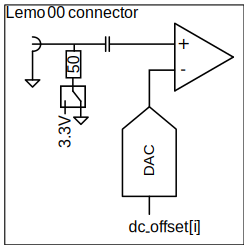
\includegraphics[width=0.3\textwidth]{figures/InputCircuit.pdf}
					}
					\caption{Input circuit for each of the input channels. \label{fig:dcoffset1}}
				\end{center} 
			\end{figure}
%%			\begin{figure}
%%				\begin{center}
%%					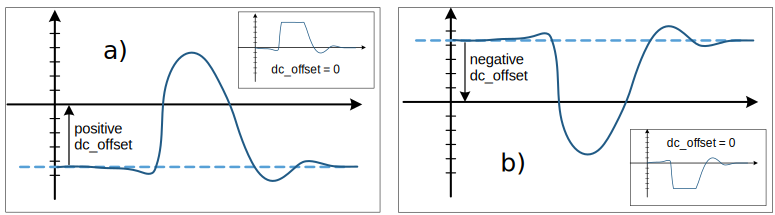
\includegraphics[width=\textwidth]{figures/dc_offset.pdf}
%%%					\caption{\textit{dc\tu offset} is used to shift the signal on each input channel such that the noise margin relative to the switching threshold is maximized.
%%					Insets of figure a) and b) show the base line of the signal with $\mathrm{\textit{dc\tu offset}}~=~0$ close to the switching threshold of the input buffer. Figure a) shows the positive pulse with $\mathrm{\textit{dc\tu offset}}~>~0$ and figure b) shows the negative pulse with $\mathrm{\textit{dc\tu offset}}~<~0$.\label{fig:dcoffset2}}
%%				\end{center}
%%			\end{figure}

			\ttvar{\prefix trigger}{trigger[\PREFIX TRIGGER\tu COUNT]}\\
			Configuration the polarity of the external trigger sources.
			These are used as inputs for the TiGer blocks and as inputs to the time measurement unit.\par

			\ttvar{\prefix tiger\tu block}{tiger\tu block[\PREFIX TIGER\tu COUNT]}
			Configuration of the timing generator (TiGer).

			\ttvar{\prefix channel}{channel[\PREFIX CHANNEL\tu COUNT]}\\
				Configure the TDC channels.

			\ttvar{\prefix low-res\tu channel}{low-res\tu channel[\PREFIX LOWRES\tu CHANNEL\tu COUNT]}\\
			\itett{
				Not applicable for \deviceName. 
			}{
				Only applicable to the xTDC4-Sciex. Configures the additional digital low-res inputs.
			}\par

			\cronvar{int}{auto\tu trigger\tu period}\\
			\cronvar{int}{auto\tu trigger\tu random\tu exponent}\\
			Create a trigger either periodically or randomly. There are two parameters $M = \text{trigger\tu period}$ and $N = \text{random\tu exponent}$ that result in a distance between triggers of $T$ clock cycles.

			\begin{align}
				T &= 1 + M + [1...2^N]\\
				&0 \leq M < 2^{32}\\
				&0 \leq N < 32
			\end{align}

			\noindent There is no enable or reset as the usage of this trigger can be configured in the TiGer block channel source field.\par

			\subsection{Structure \prefix trigger}
			\label{structtrigger}
			\cronvar{crono\tu bool\tu t}{falling}\\
			\cronvar{crono\tu bool\tu t}{rising}\\
			Select for which edges a trigger event is created inside the FPGA.
			\itett{
				The \deviceName can output measurements for one or both edges of input signals. 
			}{
				The \deviceName can output measurements with a reduced bin size of $5/6~ns = 833,\overline{3}~ps$ for one or both edges of input signals. 
				See section \ref{difficulthits} for more information on hits with varying resolution.
				Use \textsf{xtdc4\tu channel.rising} on page \pageref{structchannel} to select which edge is measured with full resolution.
				The edge that is selected for full resolution measurement must also be enabled for low resolution measurement.
			}\par

%%%%% tiger_block			

			\subsection{Structure \prefix tiger\tu block\label{cp:tigerblock}}

			\ifxHPTDC{
				\cronvar{int}{mode}\\
				Enables the desired mode of operation for the tiger.

				\begin{tabular}{lrl}
					\ttdef{TIGER \tu OFF} & 0 & no operation \\
					\ttdef{TIGER \tu OUTPUT} & 1 & output is driven with 2V amplitude. There must be no input connected \\
					\ttdef{TIGER \tu BIDI} & 2 & output is driven with 1V amplitude. Pulse rate should be low. \\
					\ttdef{TIGER \tu BIDI} & 2 & output is driven wuth 1V bidirectional pulses. $start = stop -1$\\
				\end{tabular}

				Gating blocks interpret any value that is not \ttdef{TIGER \tu OFF} as enable.	
			}{
				\cronvar{crono\tu bool\tu t}{enable}\\
				Activates the timing generator (TiGer).\par
			}
	
			\cronvar{crono\tu bool\tu t}{negate}\\
			Inverts output polarity. Default is set to false.
			\ifxHPTDC{For gating blocks, a value of false blocks inputs between start and stop, a value of true blocks outputs outside that interval.}{}\par
	
			\cronvar{crono\tu bool\tu t}{retrigger}\\
			Enables retrigger setting.\\
			If enabled the timer is reset to the value of the \textsf{start} parameter, whenever the input signal is set while waiting to reach the \textsf{stop} time.\par
	
			\cronvar{crono\tu bool\tu t}{extend}\\
			Not implemented.
	
			\ifxHPTDC{}{
				\cronvar{crono\tu bool\tu t}{enable\tu lemo\tu output}\\
				Enables the LEMO output. Drive the TiGer Signal to the corresponding Lemo connector as an output. 
				This is DC coupled, so make sure that you do not any devices connected as inputs.
				Pulses created by the TiGer are visible at the \deviceName inputs and can be measured again to get the exact timing.  
			}

			\cronvar{int}{start}\\
			\cronvar{int}{stop}\\
			\itett{
				In multiples of $4~ns$.
			}{
				In multiples of $20/3 = 6,\overline{6}~ns$
			}
			The time during which the TiGer output is set, relative to the trigger input. The parameters \textsf{start} and \textsf{stop} must fulfill the following conditions:
			\[ 0 <= start <= stop <= 2^{16}-1 \]
			If retriggering is enabled, the timer is reset to the value of the start parameter whenever the input signal is set while waiting for the stop time. \par
			
	
			\cronvar{int}{sources}\\
			A bit mask with a bit set for all trigger sources that can trigger this TiGer block. 
			Default is \textsf{\PREFIX TRIGGER\tu SOURCE\tu S}.\par
	
			\begin{tabular}{lc}
					 \ttdef{TRIGGER\tu SOURCE\tu S} & 0x00000001\\
					 \ttdef{TRIGGER\tu SOURCE\tu A} & 0x00000002\\
					 \ttdef{TRIGGER\tu SOURCE\tu B} & 0x00000004\\
					 \ttdef{TRIGGER\tu SOURCE\tu C} & 0x00000008\\
					 \ttdef{TRIGGER\tu SOURCE\tu D} & 0x00000010\\
					% \ttdef{TRIGGER\tu SOURCE\tu S1} & 0x00000020\\
					% \ttdef{TRIGGER\tu SOURCE\tu S2} & 0x00000040\\
					% \ttdef{TRIGGER\tu SOURCE\tu GATE} & 0x00000080\\
					 \ttdef{TRIGGER\tu SOURCE\tu AUTO} & 0x00004000\\
					 \ttdef{TRIGGER\tu SOURCE\tu ONE} & 0x00008000
				\end{tabular} 
	
			\subsection{Structure \prefix channel}
				\label{structchannel}
				Contains TDC channel settings.\par
	
				\cronvar{crono\tu bool\tu t}{enabled}\\
				Enable TDC channel.\par
	
				\cronvar{crono\tu bool\tu t}{rising}\\
				\itett{
					Not applicable for \deviceName.
				}{
					Select which edge of the signal is used for full resolution measurements. 
					\textsf{xtdc4\tu trigger.rising} and \textsf{xtdc4\tu trigger.falling} described on page \pageref{structtrigger} are used 
					to select which edges are recorded for low resolution measurement. 
					The edge that is selected for full resolution measurement must also be enabled for low resolution measurement.
					See section \ref{difficulthits} for more information on hits with varying resolution.
				}\par

				\itett{}{ % onyl for xTDC4
					\cronvar{crono\tu bool\tu t}{cc\tu enable}\\
					Enable carry chain TDC. This is set to \emph{true} by default and should be left unchanged. \par
	
					\cronvar{crono\tu bool\tu t}{cc\tu same\tu edge}\\
					Sets whether the carry chain TDC records the same or opposite edge as the TDC chip. 
					If the same edge is selected, that carry chain TDC acts  as a backup if the chip misses hits due to FIFO overflows or short input pulses.
					If opposite edges are selected, both edges of a pulse can be measured with reasonable resolution. See section \ref{difficulthits} for more information.\par
	
					\cronvar{crono\tu bool\tu t}{ths788\tu disable}\\
					Disable full resolution timestamps. This is set to \emph{false} by default and should be left unchanged.\par
				}
	
				\cronvar{int}{start}\\
				\cronvar{int}{stop}\\
				Veto function for grouping of hits into packets in multiples of the binsize. Only hits between start and stop are read out.
				The parameters must adhere to the following relations:
				\[
					0 <= start <= stop < 2^{ \itett{31}{30}}
				\]
	
	


%%%%%%%%%%%%%%

\ifxHPTDC{
    \section{User Data Storage}
    There is a 64~kByte flash memory on each board that users can utilize to
    store any type of data.  A typical use case would be calibration data for
    the \deviceName\ or the detectors that the device is connected to.  Also
    serial numbers of instruments built with the \deviceName\ can be stored
    here. Write operations always erase the whole memory block.\par

    \begin{description}[style=nextline]
        \item[\ttdef{USER\tu FLASH\tu SIZE 0x10000}]
        The size of the flash memory in bytes.\\

        \item[\protect{\parbox[b]{1.0\linewidth}{
            \ttvar{int}{read\tu user\tu flash(\cronvar{int}{index}, \cronvar{\uchar *}{flash\tu data}, \cronvar{\uint}{size})}\\
            \ttvar{int}{write\tu user\tu flash(\cronvar{int}{index}, \cronvar{\uchar *}{flash\tu data}, \cronvar{\uint}{size})}
        }}]
        Read from or write to the user flash of a board identified by
        \texttt{index}.  \texttt{flash\tu data} must point to a buffer
        allocated by the user.  \texttt{size} must specify the size of that
        buffer in bytes.  We recommend to always allocate a buffer of the size
        of the flash memory given by \texttt{\PREFIX FLASH\tu SIZE} to clarify
        that always the full buffer is overwritten.
    \end{description}
}{} 


    
  
          
    \chapter{Run Time Control\label{cp:readout}}  % and packet format
        \ifxHPTDC{
            	%%%%%%%%%%%%%%%%% run time control
	\section{Controlling the State of the Driver}
		\ttvar{int}{start\tu capture(}\device)\\
		Start data acquisition.\par

		\ttvar{int}{pause\tu capture(}\device)\\
		Pause a started data acquisition. 
		Pause and continue have less overhead than start and stop but don't allow for a configuration change.\par

		\ttvar{int}{continue\tu capture(}\device)\\
		Call this to resume data acquisition after a call to \textsf{\prefix pause\tu capture()}.
		Pause and continue have less overhead than start and stop but don't allow for a configuration change.\par

		\ttvar{int}{stop\tu capture(}\device)\\
		Stop data acquisition.\par

		\ttvar{int}{start\tu tiger(}\device, \cronvar{int}{index})\\
		\ttvar{int}{stop\tu tiger(}\device, \cronvar{int}{index})\\
		Start and stop the timing generator of an individual board. 
		This can be done independently of the state of the data acquisition.\par	


\section{Readout}

\ttvar{int}{read\tu hits(}\device,  \cronvar{TDCHit}{*hit\tu buf,} \cronvar{size\tu t}{size} )\\
Read a multitude of hits into a buffer provided by the user. Returns the number of read hits.\\
If grouping is enabled a single group is read. 
If the group is to large for the buffer the remaining hits of the group are discarded.\\*
If grouping is disabled, all availabe data is read up to the size of the buffer. \\
The method always returns immediately. If no hits are read it of is beneficial to call \textsf{sleep()} 
or yield the CPU to another process instead of trying again immediately.\\
Make sure to set \textsf{size} to the number of elemenst that fit into the buffer.\\*





        }{
            % NOTE: xHPTDC has a seperate file describing the readout

%%%%%%%%%%%%%%%%% run time control
\section{Run Time Control}

Once the devices are configured the following functions can be used to control
the behaviour of the devices.  All of these functions return quickly with very
little overhead, but they are not guaranteed to be thread safe.

\begin{description}[style=nextline]
    \item[\ttvar{int}{start\tu capture(}\device)]
    Start data acquisition.\par

    \item[\ttvar{int}{pause\tu capture(}\device)]
    Pause a started data acquisition. \par
    \texttt{pause} and \texttt{continue} have less overhead than start and
    stop but don't allow for a configuration change.

    \item[\ttvar{int}{continue\tu capture(}\device)]
    Call this to resume data acquisition after a call to
    \texttt{\prefix pause\tu capture()}. \par
    \texttt{pause} and \texttt{continue} have less overhead than start and
    stop but don't allow for a configuration change.

    \item[\ttvar{int}{stop\tu capture(}\device)]
    Stop data acquisition.\par
    
    \item[\protect{\parbox[b]{0.8\linewidth}{
        \ttvar{int}{start\tu tiger(}\device)\\
        \ttvar{int}{stop\tu tiger(}\device)}}]
    Start and stop the timing generator. This can be done independently of the
    state of the data acquisition.
\end{description}

%%%%%% readout
\section{Readout}
The device provides a stream of packets, that are read in batches. A batch of
packets is provided to the application, it processes them, by storing important information
in other structures. The batch that were processed need to be acknowledged, so that
the device can reuse the memory of these for the next data. That means processing
should be fast. 
\begin{lstlisting}[
    numbers=none,
]
timetagger4_read_in in;
// automatically acknowledge all data as processed
in.acknowledge_last_read = 1;
volatile crono_packet* p = read_data.first_packet;
timetagger4_read_out out;
int status = timetagger4_read(device, &in, &out);
if (status == CRONO_READ_OK) {
    while (p <= read_data.last_packet) {
        processPacket(p);
        p = crono_next_packet(p);
    }    
}
\end{lstlisting}
    
\begin{description}[style=nextline]
    \item[\ttvar{int}{acknowledge(}\device, \cronvar{crono\tu packet}{*packet)}]
    Acknowledges the processing of the last read block. This is only necessary
    if \texttt{\prefix read()} is not called with \texttt{in.acknowledge\tu
    last\tu read} set.\par
    This feature allows to either free up partial DMA space early if there
    will be no call to \texttt{\prefix read()} anytime soon.  It also allows
    to keep data over multiple calls to \texttt{\prefix read()} to avoid
    unnecessary copying of data.

    \item[\protect{\parbox[b]{\linewidth}{
        \ttvar{int}{read(}\device, \cronvar{\prefix read\tu in}{*in,} \\
        \hspace*{\labelwidth+\itemsep}\cronvar{\prefix read\tu out}{*out)}
    }}]
    Return a pointer to an array of captured data in \textsf{read\tu out}.
    The result contains a batch of packets of type \textsf{\prefix packet}.
    The batch is described by \texttt{first\tu packet} and \texttt{last\tu
    packet} in the \texttt{\prefix read\tu in} structure.
    
    \texttt{read\tu in} provides parameters to the driver. 
    A call to this method automatically allows the driver to reuse the memory
    returned in the previous call if \texttt{read\tu in.acknowledge\tu last\tu
    read} is set.\par
    Returns an error code as defined in the structure
    \texttt{\prefix read\tu out}.

    \item[\cronvar{crono\tu packet}{crono\tu next\tu packet(}\cronvar{crono\tu packet}{*packet})]
    Iterates to the next packet in the batch. 
\end{description}

\subsection{Input Structure \prefix read\tu in}
\begin{description}[style=nextline]
    \item[\cronvar{crono\tu bool\tu t}{acknowledge\tu last\tu read}]
    If set \texttt{\prefix read()} automatically acknowledges packets from the
    last read.  Otherwise \texttt{\prefix acknowledge()} needs to be called
    explicitly by the user. 
\end{description}

\subsection{Input Structure \prefix read\tu out}
\begin{description}[style=nextline]
    \item[\cronvar{crono\tu packet}{*first\tu packet}]
    Pointer to the first packet that was captured by the call of
    \texttt{\prefix read()}.

    \item[\cronvar{crono\tu packet}{*last\tu packet}]
    Address of header of the last packet in the buffer. This packet is still
    valid, all data after this packet is invalid.

    \item[\cronvar{int}{error\tu code}]
    Assignments of the error codes.\par
    \begin{tabular}{lc}
        \crondef{CRONO\tu READ\tu OK}                & \texttt{0}\\
        \crondef{CRONO\tu READ\tu NO\tu DATA}        & \texttt{1}\\
        \crondef{CRONO\tu READ\tu INTERNAL\tu ERROR} & \texttt{2}\\
        \crondef{CRONO\tu READ\tu TIMEOUT}           & \texttt{3}\\
    \end{tabular}

    \item[\cronvar{const char}{*error\tu message}]
    The last error in human readable form, possibly with additional
    information about the error.
\end{description}
    
        } 

    \chapter{Output Data Format\label{cp:packetformat}} 
        \ifxHPTDC{
            For each measured edge the \deviceName\ creates a 12 byte data structure TDCHit that contains a 64 bit timestamp in picoseconds and three fields with additional information. 

\section{Structure TDCHit}
\label{TDCHit}
\cronvar{int64\_t}{time}\\
The time stamp of the hit in picoseconds. 

If grouping is disabled the timestamps are continuously counting up from the call to \textsf{start\tu capture()}.

If grouping is enabled the timestamps are relative to the trigger or the separate zero reference of the group. 
The first TDCHit of a group has channel number 255 and provides the absolute time of the group. 
The absolute time of each of the hits can be obtained by adding this value to each of the relative timestamps.

\cronvar{uint8\_t}{channel}\\
For the first board in the system this is 0 to 7 for the TDC channels A to H. 8 or 9 for ADC data. Data from channels 8 and 9 should usually be treated as data from the same channel. 
For the other boards the channel number is incremented by $board\_id \cdot 10$.
In grouping mode the first hit of each group has channel number 255 and contains the absolute time of the group.

\cronvar{uint8\_t}{type}\\
Additional information on the type of hit recorded. See section \ref{hittypes}.

\cronvar{uint16\_t}{bin}\\
For ADC hits this contains the sampled voltage. For TDC hits the content is undefined.

\newpage
\subsection{TDCHit Types \label{hittypes}}
\newcommand{\HTYPE}{\PREFIX TDCHIT\tu TYPE\tu}

\paragraph*{Type information for TDC measurements}
If the hit is a TDC measurement on channels A to H the following flags are defined for the \textsf{type} field of the TDCHit structure:\\*
\begin{tabular}{lc}
    \crondef{\HTYPE RISING} & 0x01\\
    \indent Rising edge &\\
    \crondef{\HTYPE ERROR}  & 0x02\\
    \indent any type of error& \\
    \crondef{\HTYPE ERROR\tu TIMESTAMP\tu LOST}  & 0x04\\
    \indent Hits missing due to L1 FIFO overflow&\\
    \crondef{\HTYPE ERROR\tu ROLLOVER\tu LOST}  & 0x08\\
    \indent Invalid timestamp due to internal error&\\
    \crondef{\HTYPE ERROR\tu PACKET\tu LOST}  & 0x10\\
    \indent Hits missing due to a lost DMA packet&\\
    \crondef{\HTYPE ERROR\tu SHORTENED}  & 0x20\\
    \indent Hits missing due to a shortened DMA packet&\\
    \crondef{\HTYPE ERROR\tu DMA\tu FIFO\tu FULL}  & 0x40\\
    \indent Hits missing due to L2 FIFO overflow&\\
    \crondef{\HTYPE ERROR\tu HOST\tu BUFFER\tu FULL}  & 0x80\\
    \indent Hits missing due to host buffer overflow &\\
\end{tabular}

If hits are missing the error flag is set on the next hit from the same board that is read out.

\paragraph*{Type information for ADC measurements}
If the hit is an ADC measurement on channels 8 or 9 the following flags are defined for the \textsf{type} field of the TDCHit structure:\\*
\begin{tabular}{lc}
    \crondef{\HTYPE ADC\tu INTERNAL} & 0x01\\
    \indent ADC measurement triggered by internal strobe &\\
    \crondef{\HTYPE ADC\tu ERROR}  & 0x02\\
    \indent any type of error& \\
    \crondef{\HTYPE ADC\tu ERROR\tu INVALID\tu TRIGGER}  & 0x08\\
    \indent TRG input violated timing requirements. Data may be corrupted&\\
    \crondef{\HTYPE ADC\tu ERROR\tu DATA\tu LOST}  & 0x10\\
    \indent ADC measurement missing due to overflow of any buffer&\\
\end{tabular}

If hits are missing the error flag is set on the next hit from the same board that is read out.


 
        }{
            


\section{Output Structure crono\tu packet}

    Output of a read call list is a group of crono\tu packet structures. Which have a variable length. The structure contains the following fields.
    
	\cronvar{uint8\tu t}{channel}\\
	Index of the source channel of the data. Pseudo channel 15 is used for rollovers.\par

	\cronvar{uint8\tu t}{card}\\
	Identifies the source card in case there are multiple boards present. 
	Defaults to 0 if no value is assigned to the parameter \textsf{board\tu id} in Structure \textsf{timetagger4\tu init\tu parameters}.\par

	\cronvar{uint8\tu t}{type}\\
	The data stream consists of 32-bit unsigned data as signified by \\ CRONO\tu PACKET\tu TYPE\tu 32\tu BIT\tu UNSIGNED = 6 .\par

	\cronvar{uint8\tu t}{flags}\\
    Bit field of \textsf{TIMETAGGER4 \tu PACKET\tu FLAG\tu*}\,bits: \par
	\indent\ttdef{PACKET\tu FLAG\tu ODD\tu HITS} 1\\
	  \indent If this bit is set, the last data word in the data array consists of one timestamp only which is located \indent in the lower 32 bits of the 64-bit data word (little endian).\par
	\indent\ttdef{PACKET\tu FLAG\tu SLOW\tu SYNC} 2\\
	  \indent Timestamp of a hit is above the range of 8-bit rollover number and 24-bit hit timestamp. The group \indent is closed, all other hits are ignored.\par
	\indent\ttdef{PACKET\tu FLAG\tu START\tu MISSED} 4\\
	\indent The trigger unit has discarded packets due to a full FIFO because the data rate is too high. Starts are \indent missed and stops are potentially in wrong groups. \par
	\indent\ttdef{PACKET\tu FLAG\tu SHORTENED} 8\\
	\indent The trigger unit has shortened the current packet due to a full pipeline FIFO because the data rate is \indent too high. Stops are missing in the current packet.\par
	\indent\ttdef{PACKET\tu FLAG\tu DMA\tu FIFO\tu FULL} 16\\
	\indent The internal DMA FIFO was full. This is caused either because the data rate is too high on too many channels. Packet loss is possible.\par
	\indent\ttdef{PACKET\tu FLAG\tu HOST\tu BUFFER\tu FULL} 32\\
	\indent The host buffer was full. Might result in dropped packets. This is caused either because the data rate is too high or by data not being retrieved fast enough from the buffer. Solutions are increasing buffer size if the overload is temporary or by avoiding or optimizing any additional processing in the code that reads the data.\par

	\cronvar{uint32\tu t}{length}\\
	Number of 64-bit elements (each containing up to 2 TDC hits) in the data array. The number of hits contained is equal to 2 * length - (flags \& PACKET\tu FLAG\tu ODD\tu HITS) ? 1 : 0.\par

	\cronvar{uint64\tu t}{timestamp}\\
	Coarse timestamp of the start pulse. Values are given in multiples of \itett{packet\tu binsize contained in timetagger4\tu param\tu info}{$5/3=1.\overline{6}$\,\si{\nano\second}}.\par

	\cronvar{uint64\tu t}{data[1]}\\
	Contains the TDC hits as a variable length array (length can be zero). The user can cast the array to uint32\tu t* to directly operate on the TDC hits. For the number of hits, see length.
    Structure of one hit (32 bit):\\
	\noindent
	\begin{small}
	\begin{tabular}{|c||p{9cm}|p{1,5cm}|p{1,5cm}|}
		\hline
		bits & 31~ ~ ~ ~ ~ ~ ~ ~ ~ ~ ~ ~ ~ ~ ~ ~ ~ to ~ ~ ~ ~ ~ ~ ~ ~ ~ ~ ~ ~ ~ ~ ~ ~ ~ 8 & 7~ ~ to ~ ~ 4 & 3~ ~ to ~ ~ 0\\\hline
		content & TDC DATA & FLAGS & CHN \\\hline
	\end{tabular}
	\end{small}

	The timestamp of the hit is stored in bits 31 down to 8 in multiples of 
	\itett{binsize contained in timetagger4\tu param\tu info. \\
    }{
		$5/(3*128) = 13.0208\overline{3}$\,\si{\pico\second}
	}
    \begin{lstlisting}[numbers = none]
    uint32_t timestamp  = (hit >> 8) & 0xF;
    uint32_t flags      = (hit >> 4) & 0xF;
    uint32_t channel    =  hit       & 0xF;
    \end{lstlisting}
	
	\label{flags}
	Bits 7 down to 4 are hit flags and have the following definitions:\par
	\itett{
        Bit 7: Not applicable for the \deviceName\ and therefore always 0.\par
        
        \indent\ttdef{HIT\tu FLAG\tu COARSE\tu TIMESTAMP}~4~$\leftrightarrow$ Bit\,6\\
        \indent Bit 6: Always 1 for the \deviceName.\par
        \indent\ttdef{HIT\tu FLAG\tu TIME\tu OVERFLOW}~2~$\leftrightarrow$ Bit\,5\\
        \indent Bit 5: If set, this hit is a rollover. The time since start pulse exceeded the 24-bit range that can be encoded in a data word. This word does not encode a measurement. 
	    Instead the readout software should increment a rollover counter that can be used as the upper bits of consecutive time stamps.  
	    The counters must be reset for each packet.
	    The total offset of a hit in picoseconds can be computed by
	    \[	\Delta T_{hit} = \mathrm{(\#\ rollovers \cdot timetagger4\_static\_info.rollover\_ period + TDC\_ DATA_{hit}) \cdot timetagger4\_param\_info.binsize} \]
        \indent\ttdef{HIT\tu FLAG\tu RISING}~1~$\leftrightarrow$ Bit\,4\\
        \indent Bit 4: Set if this hit is a rising edge. Otherwise, this word belongs to a falling edge.\\
       
        \indent Bits 3 down to 0 :
	    The channel number is given in the lowest nibble of the data word. A value of 0 corresponds to channel A, a value of 3 to channel D.\\
	} {
        \indent\ttdef{HIT\tu FLAG\tu FPGA\tu MISSING}~8~$\leftrightarrow$ Bit\,7\\
        \indent\ttdef{HIT\tu FLAG\tu COARSE\tu TIMESTAMP}~4~$\leftrightarrow$ Bit\,6\\
        Bit 7, 6: Resolution of this measurement. \ifxHPTDC{}{See section \ref{difficulthits}}.\\
		\noindent
		\begin{small}
		\begin{tabular}{|c|c||l|}
			\hline
			bit 7 & bit 6 & Measurement Type \\\hline\hline
			0 & 0 &  Normal full resolution measurement.\\\hline
			0 & 1 &  Measurement performed with carry chain TDC at about \SI{150}{\pico\second} resolution.\\\hline
			1 & 0 &  Full resolution measurement that might in the wrong place in the data stream.\\\hline
			1 & 1 &  Measurement with only $5/6$\,\si{\nano\second} = $833.\overline{3}$\si{\pico\second} resolution. \\\hline
		\end{tabular}
		\end{small}
        \indent\ttdef{HIT\tu FLAG\tu TIME\tu OVERFLOW}~2~$\leftrightarrow$ Bit\,5\\
        Bit 5: Rollover. The time since start pulse exceeded the 24-bit range that can be encoded in a data word. This word does not encode a measurement. 
	Instead the readout software should increment a rollover counter that can be used as the upper bits of consecutive time stamps.  
	The counters should be reset for each packet.
	The total offset of a hit in picoseconds can be computed by
	\[	\Delta T_{hit} = \mathrm{(\#\ rollovers \cdot xtdc4\_static\_info.rollover\tu period + TDC\_ DATA_{hit}) \cdot xtdc4\_param\_info.binsize} \]
	\indent
        \indent\ttdef{HIT\tu FLAG\tu RISING}~1~$\leftrightarrow$ Bit\,4\par
        Bit 4: Set if this hit is a rising edge. Otherwise, this word belongs to a falling edge.
	The channel number is given in the lowest nibble of the data word. \\
    A value of 0 corresponds to channel A, a value of 3 to channel D.\par
	}
	
 
        }  
 
    \chapter{Code Example}  
        % SVN Info:
% $Date: 2021-01-31 20:06:56 +0100 (So, 31 Jan 2021) $
% $Rev: 1040 $
% $Author: kolja $

	The following C++ source code shows how to initializes a \deviceName\ board, configure it and loop over incoming packets.	

	If you are reading this documentation in portable document format, the source code of the C example is also embedded as an
	\txh{
		\textattachfile[color=cronlightgreen, description={Example Source Code}]{"timetagger/example.cpp"}{attachment}
		to the file. You can open it in an external viewer or save it to disk by clicking on it.
		\lstinputlisting{timetagger/example.cpp}
	}{
		\textattachfile[color=cronlightgreen, description={Example Source Code}]{xtdc/example.cpp}{attachment}
		to the file. You can open it in an external viewer or save it to disk by clicking on it.
		\lstinputlisting{xtdc/example.cpp}
	}{	
		\textattachfile[color=cronlightgreen, description={Example Source Code}]{xhptdc/example.cpp}{attachment}
		to the file. You can open it in an external viewer or save it to disk by clicking on it.

		The example code is managed as open source on GitHub at 
		\hyperlink{https://github.com/cronologic-de/xhptdc8_babel/tree/main/ug_example}{https://github.com/cronologic-de/xhptdc8\tu babel}. 
		The repository contains a complete project for Microsoft Visual Studio that you can use to compile the example.
		Examples for more programming languages such as Python and LabView will be added to the repository over time.

		\lstinputlisting{xhptdc/example.cpp}
	}
	% there were problems with underscores in file names so we removed them



    \chapter{Technical Data}    
        \ttinput{Tech.tex} 
        % SVN Info:
% $Date: 2021-01-29 22:28:41 +0100 (Fr, 29 Jan 2021) $
% $Rev: 1039 $
% $Author: kolja $

\clearpage
\section{Electrical Characteristics}

\subsection{Power Supply}

\noindent
\begin{tabularx}{\textwidth}{|c|X|c|c|c|c|}
    \hline
    Symbol & Parameter & Min & Typical & Max & Units\\
    \hline\hline
    P\subscript{total} & Total power consumption & & & \ifxHPTDC{20}{10}& \si{\watt}\\
    \hline
    VCC\subscript{3.3} & PCIe \SI{3.3}{\volt} rail power supply voltage &3.1&3.3&3.5& \si{\volt}\\
    \hline
    I\subscript{3.3} & PCIe \SI{3.3}{\volt} rail input current & & &\txh{650}{600}{600}& \si{\milli\ampere}\\
    \hline
    VCC\subscript{12} & PCIe \SI{12}{\volt} rail power supply voltage &11.1&12.0&12.9& \si{\volt}\\
    \hline
    I\subscript{12} & PCIe \SI{12}{\volt} rail input current & & & \txh{550}{650}{1500} & \si{\milli\ampere}\\
    \hline
    VCC\subscript{aux} & PCIe 3.3\,V\subscript{Aux} rail power supply voltage &&3.3&& \si{\volt}\\
    \hline
    I\subscript{aux} & PCIe 3.3\,V\subscript{Aux} rail input current &&0&& \si{\milli\ampere}\\
    \hline
\end{tabularx}

\subsection{TDC Inputs} \label{din:tdcinputs}
The \deviceName's inputs are single-ended AC-coupled with 50\,Ω termination.

\noindent
\begin{tabularx}{\textwidth}{|c|X|c|c|c|c|}
    \hline
    Symbol & Parameter & Min & Typical & Max & Units\\
    \hline\hline
    V\subscript{Base} & Input Baseline & 0 & & 5 & \si{\volt}\\
    \hline
    V\subscript{Threshold} & Trigger Level & V\subscript{Base} $-$ \dcminabs & & V\subscript{Base} + \dcmax & \si{\volt}\\
    \hline
    |ΔV\subscript{min}| & Magnitude of minimal pulse height & \ifxHPTDC{100}{10} & & & \si{\milli\volt}\\
    \hline
    \itett{
        t\subscript{Pulse} & Pulse Length\newline
            \hfill --1.25G\newline
            \hfill --2.5G\newline
            \hfill --5G\newline
            \hfill --10G
        & \makecell[tc]{\mbox{}\\0.8\\0.4\\0.2\\0.1} & 5 & 200 & \si{\nano\second}
    }
    {
        t\subscript{Pulse} & Pulse Length & 2 & 5 & 200 & \si{\nano\second}
    }\\
    \hline
    t\subscript{Rise} & Pulse Edge 20\% to 80\%  &  &  & 10 & \si{\nano\second}\\
    \hline
    t\subscript{Fall} & Pulse Edge 80\% to 20\%  &  &  & 10 & \si{\nano\second}\\
    \hline
    Z\subscript{P} & Input Impedance && 50 && Ω\\
    \hline
    I\subscript{Term} & Termination Current & --50 & --20 & 50 & \si{\milli\ampere}\\
    \hline
\end{tabularx}

All inputs are AC-coupled. The inputs have very high input bandwidth
requirements and therefore there are no circuits that provide over-voltage
protection for these signals.  Any voltage on the inputs above \SI{5}{\volt}
or below \SI{-5}{\volt} relative to the voltage of the slot cover can result
in permanent damage to the board.\par Keep in mind, that the input baseline
\textsf{V\subscript{Base}} is affected by the ratio of pulse length
\textsf{t\subscript{Pulse}} to average pulse distance (for continuous signals
the term is called duty cycle).\par

\ifxHPTDC{
    All digital inputs can output AC coupled pulses from the TiGer.  Special
    care should be taken not to enable the TiGer output when sensitive
    equipment is connected that could be damaged by the pulses. 
}{
    Make sure not to drive the inputs when the connector is configured as a
    TiGer output.\par 
}
See Section \ref{cp:tiger}. 

%%%%%%%%%%% ADC input
\ifxHPTDC{
    \newpage
    \subsection{ADC Inputs}
    The ADC input is DC coupled to a differential termination voltage of
    400\,mV.  This means that the actual voltage seen by the ADC will depend on
    the output impedance of the source that is driving the input.\par
    \noindent
    \begin{tabularx}{\textwidth}{|c|X|c|c|c|c|}
        \hline
        Symbol & Parameter & Min & Typical & Max & Units\\
        \hline\hline
        V\subscript{in} & Input voltage & --2.0 &  & 2.5 & V \\
        \hline 
        V\subscript{term} & Termination voltage & & 0.4 & & V \\
        \hline 
        Z\subscript{in} & Input Impedance & & 50  & & Ω \\
        \hline
    \end{tabularx}

    %%%%%%%%%%% clock input		
    \subsection{Clock input J2}
    The clock input J2 is single ended and AC coupled.\\*
    \noindent
    \begin{tabularx}{\textwidth}{|c|X|c|c|c|c|}
        \hline
        Symbol & Parameter & Min & Typical & Max & Units\\
        \hline\hline
        V\subscript{p-p} & Peak to Peak voltage & 1 &  & 3.3 & V \\
        \hline 
        V\subscript{cm} & Common mode voltage voltage &--3 &   & 3 & V \\
        \hline 
        V\subscript{tck} & Clock termination voltage & & 0 &  & V \\
        \hline 
        Z\subscript{in} & Input Impedance & & 50  & & Ω \\
        \hline 
        D\subscript{J2} & Duty cycle & 45 & 50 & 55 & \% \\
            \hline 
            f\subscript{J2}& Frequency &  & 10 &  & MHz \\
        \hline
    \end{tabularx}
}{}

\newpage
\section{Information Required by DIN EN 61010-1}
\subsection{Manufacturer\label{cp:manu}}

The \deviceName\ is a product of:\

\begin{quote}
    cronologic GmbH \& Co. KG\\
    Jahnstra\ss{}e 49\\
    60318 Frankfurt\par
    Germany
    \noindent HRA 42869 beim Amtsgericht Frankfurt/M\par
    \noindent VAT-ID: DE235184378 \\*
    \noindent PCI Vendor ID: 0x1A13
\end{quote}

\subsection{Intended Use and System Integration}
The devices are not ready to use as delivered by cronologic. It requires the
development of specialized software to fulfill the application of the
end-user. The device is provided to system integrators to be built into
measurement systems that are distributed to end users. These systems usually
consist of the \deviceName, a main board, a case, application software and
possibly additional electronics to attach the system to some type of detector.
They might also be integrated with the detector.\par

The \deviceName\ is designed to comply with DIN EN 61326-1 when operated on a
PCIe compliant main board housed in a properly shielded enclosure.  When
operated in a closed standard compliant enclosure the device does not pose any
hazards as defined by EN 61010-1.\par

Radiated emissions, noise immunity, and safety highly depend on the quality of
the enclosure.  It is the responsibility of the system integrator to ensure
that the assembled system is compliant to applicable standards of the country
that the system is operated in, especially regarding user safety and
electromagnetic interference. \par
    
When handling the board, adequate measures must be taken to protect the
circuits against electrostatic discharge (ESD). All power supplied to the
system must be turned off before installing the board.

\subsection{Environmental Conditions for Storage}
The board shall be stored between operation under the following conditions:

\noindent
\begin{tabularx}{\textwidth}{|c|X|c|c|c|c|}
    \hline
    Symbol & Parameter & Min & Typical & Max & Units\\
    \hline\hline
    T\subscript{store} & ambient temperature & --30 && 60 & \si{\degreeCelsius}\\
    \hline
    RH\subscript{store} & relative humidity at 31$^{\circ}$C noncondensing & 10 && 70 & \%\\
    \hline
\end{tabularx}

\clearpage
\subsection{Environmental Conditions for Operation}
The board is designed to be operated under the following conditions:

\noindent
\begin{tabularx}{\textwidth}{|c|X|c|c|c|c|}
    \hline
    Symbol & Parameter & Min & Typical & Max & Units\\
    \hline\hline
    T\subscript{oper} & ambient temperature & 5 && 40 & \si{\degreeCelsius}\\
    \hline
    RH\subscript{oper} & relative humidity at 31$^{\circ}$C & 20 && 75 & \%\\
    \hline
\end{tabularx}

WARNING: Do not connect any DC-coupled inputs to a channel while the TiGer of
that channel is configured as an output (see Section~\ref{cp:tiger}).  Doing
so could permanently damage the \deviceName\ and the external hardware.

\subsection{Cooling}
The \deviceName\ in its base configuration has passive cooling that requires a
certain amount of air-flow.  If the case design can't provide enough air-flow
to the board, a slot cooler like Zalman ZM-SC100 can be placed next to the
board.  Active cooling is also available as an option for the board.


\subsection{Recycling}
cronologic is registered with the ``Stiftung Elektro-Altgeräte Register''
as a manufacturer of electronic systems with Registration ID DE 77895909.\par
The \deviceName\ belongs to category 6, ``Kleine Geräte der Informations- und
Telekommunikationstechnik für die ausschließliche Nutzung in anderen als
privaten Haushalten.''  Devices sold before 2018 belong to category 9,
``Überwachungs und Kontrollinstrumente für ausschließlich
gewerbliche Nutzung.'' The last owner of a \deviceName\ must recycle it,
treat the board in compliance with \S{}11 and \S{}12 of the German ElektroG,
or return it to the manufacturer's address listed on Page~\pageref{cp:manu}.
    
    \chapter{Revision History} 
        \noindent
        User Guide \hyperlink{ugrev}{\ugrev} as of 2024-05-21\\  % needs also be updated in UgRev.tex
    %	\\
        cronologic GmbH \& Co. KG\\
        Jahnstraße 49\\
        60318 Frankfurt am Main\\Germany\\
        \ttinput{FwRev.tex}
        \ifxHPTDC{\section{Driver \& Applications}
\begin{tabularx}{\textwidth}{|c|c|X|}
    \hline
    Revision & Date & Comments\\
    \hline\hline
    \hypertarget{drvrev}{1.0.1} & 2021-12-08 & primary release\\
    \hline
 
\end{tabularx}}{\section{Driver \& Applications} \label{sec:rev_driver_applications}
\begin{tabularx}{\textwidth}{|c|c|X|}
    \hline
    Revision & Date & Comments\\
    \hline\hline
    \hline
    \hypertarget{drvrev}{1.9.0} & 2023-07-10 &
    \makecell[l] {
       added quantization to timetagger4\_param\_info structure \\*
       Code refactorization\\*   
    }\\   
    \hline
    {1.8.3} & 2023-06-07 &
    \makecell[l] {
        Minor bug fixes\\*
        Code refactorization\\*        
    }\\
    \hline
    {1.8.2} & 2023-05-17 &
    \makecell[l] {
        Added bounds and checks for various parameters\\*         
    }\\
    \hline
    {1.8.1} & 2023-05-09 &
    \makecell[l] {
     Renamed autotrigger mode to continuous mode  \\*  
    }\\
    \hline
    {1.8.0} & 2023-05-05 &
    \makecell[l] {
        Added configurable input delay\\*
    }\\
    \hline
    {1.7.0} & 2023-04-18 &
    \makecell[l] {
        Board Revision 7 support\\* 
        TimeTagger4 : added autotrigger mode\\*
    }\\
    \hline
    {1.4.5} & 2022-10-17 &
    \makecell[l] {
        kernel driver v1.4.2 for xTDC4 only\\* 
        (fixes crash on Windows for Thunderbolt hot-plug)\\*
    }\\
    \hline
    {1.4.4} & 2022-06-27 &
        kernel driver v1.4.1\\
    \hline
    1.4.2 & 2021-07-28 &
    \makecell[l]{
        Firmware updated \\*
        ReadoutGUI added/updated \\*
        User guide example added/updated \\*
    }\\
    \hline
    {1.4.1} & 2019-11-11 & x64 32 mode issues fixed\\
    \hline
    {1.4.0} & 2019-06-04 & Improved Windows 10 support\\
    \hline
    {1.3.0} & 2019-01-23 & Added Windows 10 support\\
    \hline
\end{tabularx}} 
        % Also update date and version in User_Guide.tex

\section{User Guide}
\begin{tabularx}{\textwidth}{|c|c|X|}
    \hline
    Revision & Date & Comments \\
    \hline\hline
    \hypertarget{ugrev}{1.8.9} & 2023-07-10 &
    \makecell[l]{
        TimeTagger4 Userguide rework
    }\\
    \hline
    {1.8.8} & 2023-03-15 &
    \makecell[l]{
        new TimeTagger4 variants -1.25G to -10G added        
    }\\
    \hline
    1.8.7 & 2022-11-24 &
    \makecell[l]{
        Firmware revision notes updated
    }\\
    \hline
    {1.8.6} & 2022-11-23 &
    \makecell[l]{
        Spelling and grammar corrections \\*
        new example source code for xHPTDC8 
    }\\
    \hline
    {1.8.5} & 2021-12-17 &
    \makecell[l]{
        Clarifications related to TimeTagger4 configuration.
    }\\
    \hline    
    {1.8.4} & 2021-12-08 &
    \makecell[l]{
        Updated grouping structure in xHPTDC8 API
    }\\
    \hline    
    {1.8.3} & 2021-07-28 &
    \makecell[l]{
        Updated firmware revision history
    }\\
    \hline
    {1.8.2} & 2021-04-23 &
    \makecell[l]{
        Added software trigger and \tu SYNC trigger sources for xHPTDC8 \\*
        Corrected 3.3V power requirement for xHPTDC8 \\*
        Changed types with fixed bit width to \textsf{stdint.h} for xHPTDC8 \\*
        Added user flash functions for xHPTDC8 \\*
    }\\
    \hline
    {1.8.1} & 2021-04-09 &
    \makecell[l]{
        Many corrections and updates to the xHPTDC8 API
    }\\
    \hline
    {1.8.0} & 2021-03-22 &
    \makecell[l]{
        Added xHPTDC8 User Guide
    }\\
    \hline
    {1.7.0} & 2021-02-04 & 
    \makecell[l]{
        Combined User Guide for -1G and -2G \\
        Added characteristics for INL, DNL and Time Base \\
        Reordered sections for clarity \\
        Error corrections for rollovers, binsize and range \\
        Added figure \ref{fig:matrix} (TiGer matrix) \\
        Corrected board revision \\
    }\\
    \hline
    \itett{1.3.0}{1.6.0} & 2019-06-05 & API clarifications \\
    \hline
\end{tabularx}  


    \ifxHPTDC{}{
    \phantomsection
    \addcontentsline{toc}{chapter}{Erratum}
    \chapter*{Erratum}
        We found undesired behaviour for Gen\,1 devices of the \deviceName.\par
If there are three or more edges close together (within \SI{6.6}{\nano\second}) and the user did only enable rising or falling edges but not both, some of the edges are reported with the wrong polarity. \itett{}{To trigger this behaviour you need to violate the \textsf{t\subscript{DPfull}} parameter of the board that states that for full resolution you may not have more than one pulse within a \SI{5}{\nano\second} interval.}\

If your configuration enables both edges all output data is correct.\
If you only need one type of edge (rising or falling) there are three simple workarounds:\ 

\begin{itemize}
    \item[a)] update the Firmware of your Gen\,1 device to \itett{svn1187}{svn1192} or later.
    \item[b)] enable both edges.\par
    All output words will be correct and your software can ignore all data that doesn't have the desired polarity.
    \item[c)] enable only the desired edge polarity\par 
    Ignore the polarity flag in the output data. You can trust that only edges with the desired polarity are output, even if the flag in the data word states the wrong polarity.
\end{itemize}
    }
\end{document}"

% or define it here
%\newcommand{\deviceName}{TimeTagger4}
%\newcommand{\deviceName}{xTDC4}

  
\ifthenelse{\isundefined{\deviceName}}{ 
	\message {\\ WARNING: Undefined device name, TimeTagger4 used}
	\newcommand{\deviceName}{TimeTagger4}}{}
\message{\\Device name is \deviceName }


%output the first option for the TimeTagger, the second one otherwise
% example: 
% \itett{THIS IS A TimeTagger4}{THIS IS NOT}
\ifthenelse{\equal{\deviceName}{TimeTagger4}}{\newcommand{\itett}[2]{#1}}{\newcommand{\itett}[2]{#2}}
\itett{\message{\\TIMETAGGER\\}}{\message{\\NO TIMETAGGER\\}}

% output code only for the xHPTDC8 
% example: 
% \ifXHPTDC{THIS IS AN xHPTDC8} {THIS IS NOT}
% NOTE: Macro names may not contain digits
\ifthenelse{\equal{\deviceName}{xHPTDC8}} {\newcommand{\ifxHPTDC}[2]{#1}}{\newcommand{\ifxHPTDC}[2]{#2}}
\ifxHPTDC{\message{\\XHPTDC8\\}}{\message{\\NO XHPTDC\\}}
 
  
 
% output code for the TimeTagger4, xTDC4 or xHPTDC8
% example: 
% \txh{THIS IS A TimeTagger4}{THIS IS AN xTDC4}{THIS IS AN xHPTDC8}
\itett{\newcommand{\txh}[3]{#1}}{\ifxHPTDC{\newcommand{\txh}[3]{#3}} {\newcommand{\txh}[3]{#2}}}
 
\txh{ % TimeTagger4
	\message{Generating User Guide for TimeTagger4}
	\newcommand{\ttinput}[1]{\input{timetagger/#1}}
	\newcommand{\titlefile}{"figures/TT4_title.pdf"}
	\newcommand{\prefix}{timetagger4\tu}
	\newcommand{\PREFIX}{TIMETAGGER4\tu}
}{ % xTDC4
	\message{Generating User Guide for xTDC4}
	\newcommand{\ttinput}[1]{\input{xtdc/#1}}
	\newcommand{\titlefile}{"figures/xTDC4_title.pdf"}
	\newcommand{\prefix}{xtdc4\tu} 
	\newcommand{\PREFIX}{XTDC4\tu}
} 
{ % xHPTDC8
	\message{Generating User Guide for xHPTDC8}
	\newcommand{\ttinput}[1]{\input{xhptdc/#1}}
	\newcommand{\titlefile}{"figures/xHPTDC8_title.pdf"}
	\newcommand{\prefix}{xhptdc8\tu}
	\newcommand{\PREFIX}{XHPTDC8\tu}
} 

\ifxHPTDC{
	\newcommand{\longlong}{int64\tu t} 
	\newcommand{\uint}{uint32\tu t}
	\newcommand{\ushort}{uint16\tu t}
	\newcommand{\uchar}{uint8\tu t}	
}{
	\newcommand{\longlong}{\tu \tu int64}
	\newcommand{\uint}{unsigned int}
	\newcommand{\ushort}{unsigned short}
	\newcommand{\uchar}{unsigned char}	
}


\hyphenation{Time-Tagger xTDC xHPTDC cronologic}


\newcommand{\ttvar}[2]{\noindent\textsf{\textbf{\textcolor{crongrey}{#1} \prefix #2}}}%for variable declaration
\newcommand{\ttdef}[1]{\noindent\textsf{\textcolor{crongrey}{\#{}define} \PREFIX #1}}%for definitions

\newcommand{\ugrev}{{1.8.6rc}}
%%%%%%%%%%%%%%%%%%%%%%%%%%%%%%%%% 
 
\begin{document}  
\cronofront{\titlefile}
 
% 
	\chapter{Introduction}
		\ttinput{Intro.tex}

	\chapter{Hardware}  
		\label{sec:installation-of-board}

\ifxHPTDC{}{
    The \deviceName\ is available as a PCIe plugin board (variant ``-PCIe'', see \hyperlink{cp:ordering_information}{Ordering Information}) or as a desktop solution (variant ``-TBT'').
    %The two variants are shown in Figure~\ref{fig:boards-overview}.
    For a detailed overview of the hardware of the TBT-variant, please refer to our respective \href{https://docs.cronologic.de/projects/tbt2pcie/}{online user guide}.

    % \begin{figure}[htb]
    %     \centering
    %     \itett{
    %         \includegraphics[width=0.9\textwidth]{timetagger/figures/board-overview}
    %     }{

    %         \includegraphics[width=0.9\textwidth]{xtdc/figures/board-overview}
    %     }
    %     \caption{Overview of the PCIe (left) and the TBT (right) variant of the \deviceName.\textcolor{red}{TODO}}
    %     \label{fig:boards-overview}
    % \end{figure}
}

\section{Installing the PCIe Board}
The \deviceName\ board can be installed in any PCIe-CEM slot with x1 or more
lanes.  Make sure that the PC is powered off and that the main power connector is disconnected while installing the board.\par

%
\section{\deviceName\ Inputs and Connectors}
    Figure~\ref{fig:bracket} shows the location of the inputs on the slot
    bracket.  %
    %
    \begin{figure*}[htb]
        \centering
            \ifxHPTDC{
                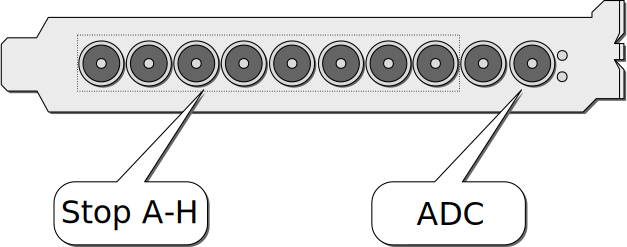
\includegraphics[width=0.6\textwidth]{%
                    figures/xHPTDC8_Slotblende.pdf}
            }{
                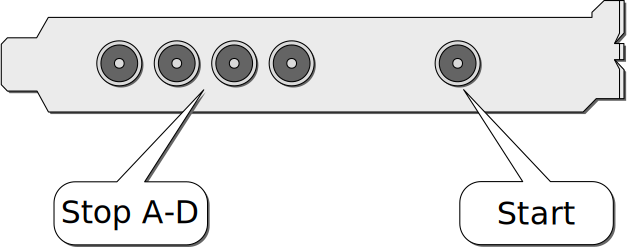
\includegraphics[width=0.6\textwidth]{%
                    figures/xTDC4_Slotblende.pdf}
            }
            \caption{
                Input connectors of the \deviceName\ on the PCIe
                bracket.%
                \ifxHPTDC{
                    Note, the TRG connector acts as a trigger only for the
                    ADC channel, not the TDC channels (see Section~\ref{adc}).
                }{}
                \label{fig:bracket}
            }
    \end{figure*}
    %
    \begin{figure*}[htb]
        \centering
            \ifxHPTDC{
                \includegraphics[width=0.3\textwidth]{%
                    xhptdc/figures/InputCircuit.pdf}
            }{
                \includegraphics[width=0.3\textwidth]{%
                    figures/InputCircuit.pdf}
            }
            \caption{
                Input circuit for each of the input
                channels.
                \ifxHPTDC{
                    Note, the TRG connector acts as a trigger only for the
                    ADC channel, not the TDC channels (see Section~\ref{adc}).
                }{}
                \label{fig:inputcirc}
            }
    \end{figure*}
    %

    LEMO-00 connectors are used for input connection. The inputs are AC-coupled
    and have an impedance of 50\,Ω.  A schematic of the input circuit is shown
    in Figure \ref{fig:inputcirc}.  The digital threshold for any input can be
    adjusted to comply with a multitude of single-ended signaling standards. 
    The threshold can also be used to configure the input for either positive
    or negative pulses.
    
    The connectors can also be used as outputs. 
    \ifxHPTDC{AC-coupled}{DC-coupled} output pulses for automatic internal
    triggering and control of external devices can be generated using the
    TiGer timing pattern generator. See Section~\ref{cp:tiger} for details on
    the TiGer. 
    \ifxHPTDC{
        Furthermore, three inter-board connectors can be found near the top
        edge of the \deviceName\ board, as displayed in
        Figure~\ref{fig:schematics}.  Connector J25 is reserved for future
        use. The pinout of connector J12 is shown in Table~\ref{J12} and the
        pinout of connector J6 is depicted in Table~\ref{J6}.
        Connector J2 is a coax clock input that must receive a 10~MHz clock if
        multiple boards are used together as described in
        Section~\ref{multiboard}.
    }{%TT4 & xTDC4
        Furthermore, for Gen\,1 boards three inter-board connectors can be
        found near the top edge of the \deviceName\ board, as displayed in
        Figure~\ref{fig:schematics}. Connector J25 is reserved for future
        use. The pinout of connector J12 is shown in Table~\ref{J12} and the
        pinout of connector J6 is depicted in Table~\ref{J6}. \textbf{Gen\,2
        boards do not possess these three connectors}.
    }
    %
        \begin{figure*}[htb]
            \centering
                \ifxHPTDC{
                    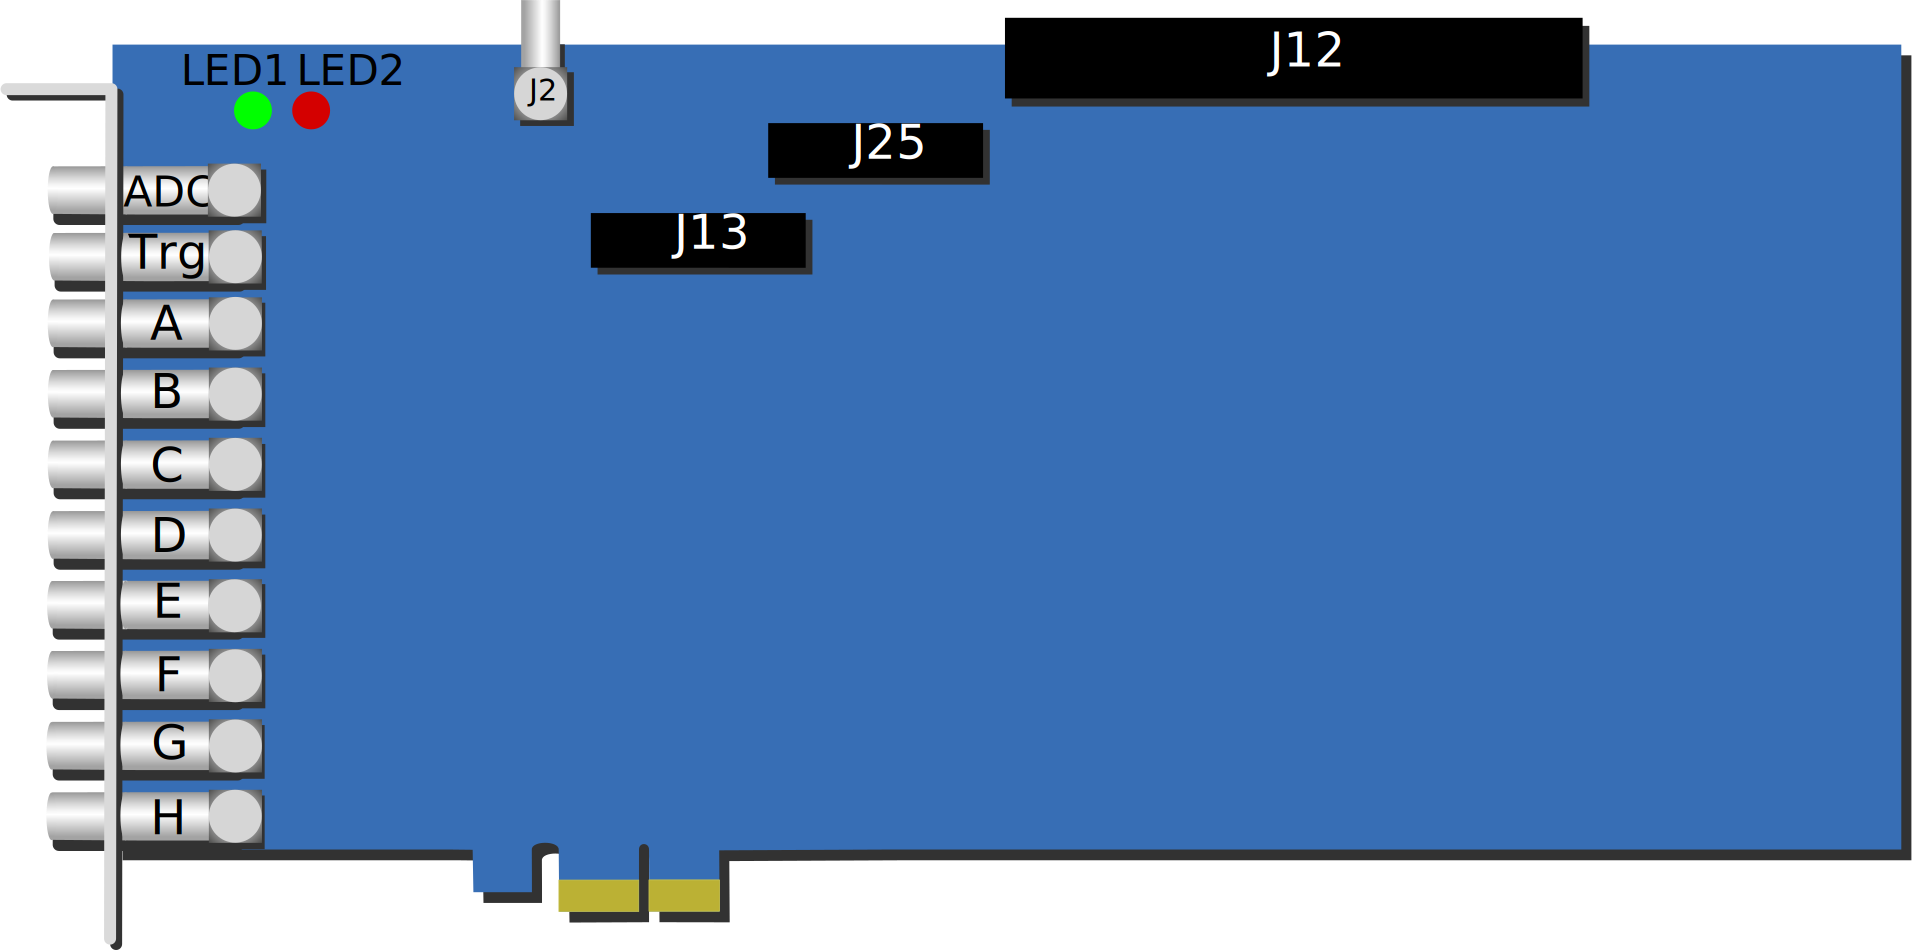
\includegraphics[width=0.7\textwidth]{%
                        xhptdc/figures/xHPTDC8_schematic.pdf}
                }{
                    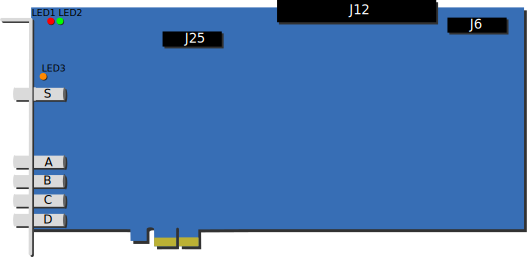
\includegraphics[width=0.7\textwidth]{%
                        figures/xTDC4_schematic.pdf}
                }
                \caption{Schematic view of \adeviceName\ Gen\,1 board showing
                    the inter-board connectors.\label{fig:schematics}}
        \end{figure*}
    %

    \begin{table}
    \begin{small}
        \centering
            \begin{tabular}{|c|c|}
                \hline
                Pin & Name\\
                \hline\hline
                1, 2 & GND\\
                \hline
                3, 4 & external CLK in N, external CLK in P\\
                \hline
                5, 6 & GND\\
                \hline
                7, 8 & reserved/NC\\
                \hline
                9, 10 & GND\\
                \hline
                11, 12 & reserved/NC\\
                \hline
                13, 14 & GND\\
                \hline
                15, 16 & reserved/NC\\
                \hline
                17, 18 & GND\\
                \hline
                19, 20 & reserved/NC\\
                \hline
                21, 22 & GND\\
                \hline
                23, 24 & reserved/NC\\
                \hline
                25, 26 & GND\\
                \hline
                27, 28 & reserved/NC\\
                \hline
                29, 30 & GND\\
                \hline
                31, 32 & reserved/NC\\
                \hline
                33, 34 & GND\\
                \hline
            \end{tabular}
            \caption{Pinout of connector J12.}
            \label{J12}
    \end{small}
    \end{table}

    \begin{table}
    \begin{small}
        \centering
            \begin{tabular}{|c|c|}
                \hline
                Pin & Name\\
                \hline\hline
                1 & +\SI{3.3}{\volt}\\
                \hline
                2 - 9 & reserved/NC\\
                \hline
                10 & GND\\
                \hline
            \end{tabular}
            \caption{Pinout of connector J6.}
            \label{J6}
    \end{small}
    \end{table}

%%%%%%%%%%%%%%% LEDs
\ifxHPTDC{
    \section{Status LEDs}
    Four status LEDs are present on the board. Two are located on the PCB, two more on the PCIe bracket.

    \begin{itemize}
        \item On the PCIe bracket (see Figure~\ref{fig:bracket}): The top LED  lights up green after the board is initialized. The bottom LED lights up briefly while the board is being configured and continuously while the card is capturing.
        \item On the PCB (see Figure~\ref{fig:schematic}): The red LED2 lights up during the configuration of the FPGA and turns off afterward. If it stays permanently lit, the configuration failed. The green LED1 lights up briefly while the board is being configured.
    \end{itemize}
}
{
    \section{Status LEDs of the PCIe boards}
    Three status LEDs are present on the board, as seen in 
    Figure~\ref{fig:schematics}.
    \begin{itemize}
        \item LED1 lights up red during the configuration of the FPGA
            and turns off afterward. If it stays permanently lit, the
            configuration failed.
        \item LED2 lights up green after the board is initialized by the
            driver and turns off when the device is closed by the
            software.
        \item LED3 lights up green when capture is started, yellow after
            the first start signal was detected and red when groups are
            missing.
    \end{itemize}
}

%%%%%%%%%%%%%%% multiboard
\ifxHPTDC{
    \section{Synchronizing multiple boards}
        \label{multiboard}
        If more than eight TDC inputs are required, up to six boards can be
        synchronized within a system. 
        
        The \deviceName\ API described in Chapter~\ref{cp:api} manages up to
        six boards automatically and provides a single data stream that
        contains sorted hit data from all boards in chronological order. 
        Channel A of each board is assigned channel number $\texttt{board\tu
        index} \times 10$.  The \texttt{board\tu index} is assigned to the
        boards in the order of the serial numbers starting at 0.

        \subsection{Connecting multiple boards}
            The boards must each receive a common \SI{10}{\mega\hertz} clock
            signal on connector J2. The connector is inside the PC enclosure. 
            Connectors J12 of all boards must be connected with a flat band
            cable with a terminator at each end.  Cable and Terminator are
            available from cronologic. See Figure~\ref{fig:multiboard} for a
            wiring example.  %
            \begin{figure*}[htb]
                \centering
                    \includegraphics[width=1\textwidth]{
                        xhptdc/figures/multiboard.pdf}				
                    \caption{Synchronizing multiple boards with a
                        ClockBox.\label{fig:multiboard}}
            \end{figure*}
            %
        \subsection{ClockBox}
            For systems of up to four boards, cronologic offers the ClockBox
            product that conveniently makes four clock signals available
            inside the PC enclosure. For use with the \deviceName, jumper JP3
            of the ClockBox must be set as shown in Figure~\ref{fig:clockbox}
            in order to set the clock frequency to \SI{10}{\mega\hertz}. 
            %
            \begin{figure*}[htb]
                \centering
                    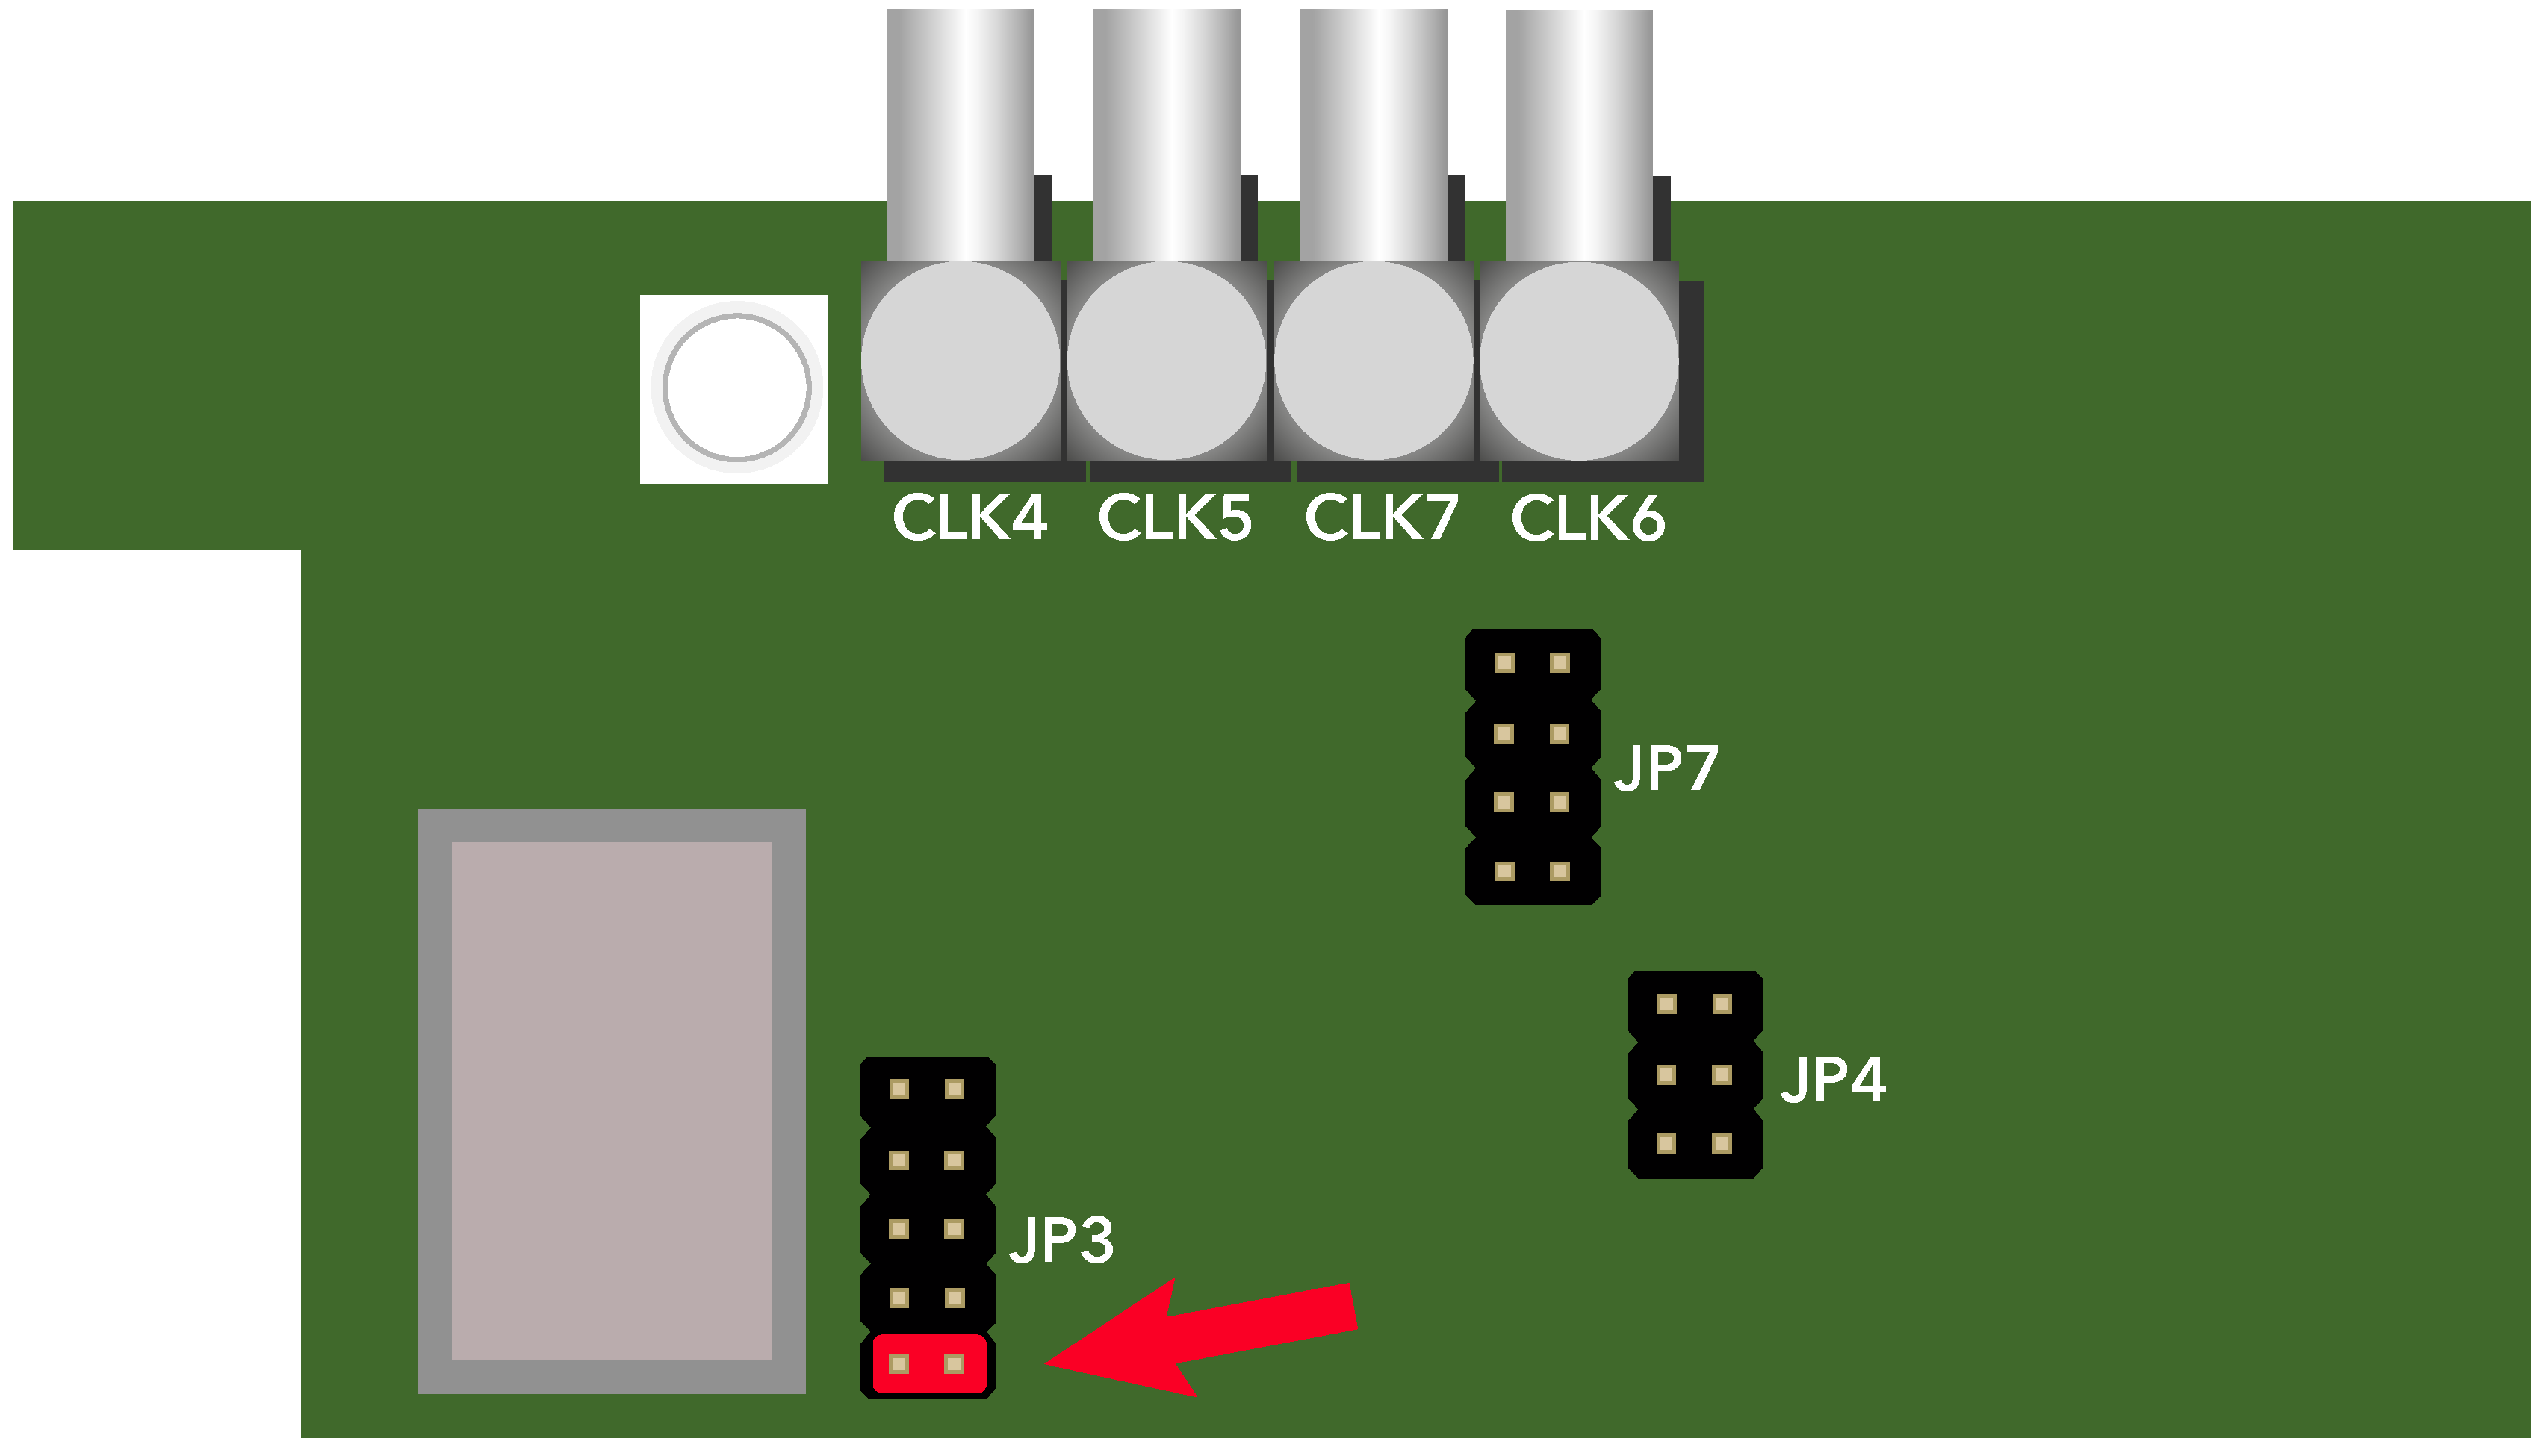
\includegraphics[width=0.5\textwidth]{
                        xhptdc/figures/clockbox.pdf}				
                    \caption{ClockBox jumper setting for
                        \SI{10}{\mega\hertz}.\label{fig:clockbox}}
            \end{figure*}
            %
        
        \subsection{Crates for multiple boards}
            Most PC mainboards don't have enough PCIe slots to support six
            \deviceName s.  We offer an external enclosure called ``Ndigo
            Crate'' that uses PCIe-over-cable technology to extend the number
            of available slots in a system.  The extension is fully
            transparent to the host system. There are no additional drivers
            required.  Please see the
            \href{https://www.cronologic.de/products/pcie/pcie-crates}{%
                product page} at our website \url{www.cronologic.de}.
}{}




    




	\chapter{\deviceName\ Functionality}
		\txh{ %TimeTagger Version
The \deviceName\ is a ``classic'' common start time-to-digital converter. 

It records the time difference between a leading or trailing edge on the start input to the leading and trailing edges of the stop inputs. 
Rising and falling edges of the stop channels A-D can be enabled individually. 
The measurements are quantized as shown in section \ref{sec:features}. 
The timestamps are recorded in integer multiples of the corresponding bin size.
Transitions of the input signals are called hits. To reliably detect hits the signal has to be stable for more than one quantisation interval before and after the edge.  
Triggers on the start channel must not occur less than \SI{5}{\nano\second} apart. The \deviceName\ records events without dead time at a readout rate of about 48\,MHits/s for Gen\,1 and 60\,MHits/s for Gen\,2.
} { %xTDC4 and xHPTDC8 Version
The \deviceName\ is a ``classic'' common start time-to-digital converter. 

It records the time difference between leading or trailing edges on the start input and the stop inputs. 
Each stop channel A-D can be enabled individually. 
The standard deviation of the timestamps is approx. \SI{8}{\pico\second}. 
The timestamps are recorded in integer multiples of a bin size of $5000/(3\cdot 128)$ = $13.0208\overline{3}$\,\si{\pico\second}. 
The data acquisition can be limited to rising or falling signal transitions. 

The maximum trigger rate on the start channel is \SI{4}{\mega\hertz}.

\subsection{Handling of Difficult Hits}
    \label{difficulthits}
    Transitions of the input signals are called hits. To measure all hits with the maximum resolution the hits must fulfill all criteria set forth in this document.
    However, the \deviceName does include mechanisms to provide as much information as possible for hits that fall out of these specs.

    To reliably detect hits the signal has to be stable for at least \SI{900}{\pico\second} before and after the edge that is to be measured. 
    Pulses as short as \SI{250}{\pico\second} are usually detected at full resolution but have a significant chance to be assigned to the wrong group or appear out of order. 
    For these hits bit 7 in the data word is set. See section \ref{flags} for more information on the data format.

    Between multiple hits on a stop channel a dead time of approximately \SI{5}{\nano\second} is required for full resolution. 
    Hits that are closer together will only be reported with a resolution of $5/6$\,\si{\nano\second} = $833\overline{3}$\,\si{\pico\second}. For these hits both bits 6 and 7 are set.

    Data is copied from the 15-entry L0 FIFO to the larger downstream FIFOs at a rate of about \SI{12}{\mega\hertz} per channel. 
    If the L0 FIFO overflows the high resolution measurement of some hits will be discarded. 
    In this case a measurement from an alternative TDC will be used that has a resolution of about \SI{150}{\pico\second}. 
    For these hits bit 6 in the data word will be set
} { %xHPTDC8 version
    The \deviceName\ is a streaming time-to-digital converter. It records the timestamps of changes at the inputs A-H in an infinite stream. 
    A flexible grouping mode is available that can emulate common-start or common-stop behaviour. See section \ref{grouping} for details.

    For each channel, it can be selected individually whether rising or falling edges are recorded. It is not possible to record both edges of the same channel. 
    The timestamps are recorded in integer multiples of a bin size of $5000/(3\cdot 128)$ = $13.0208\overline{3}$\,\si{\pico\second}. 
    There must be at least \SI{5}{\nano\second} between consecutive hits on the same input channel to be detected reliably. 
    The \deviceName\ records events without dead time at a readout rate of about $48$\,MHits/s.
} 
		\section{Grouping and Events}
\label{grouping}
\ifxHPTDC{
    If \textsf{config.tdc\tu mode} is set to \textsf{\PREFIX TDC\tu MODE\tu CONTINOUS} the TDC will operate in grouping mode. 
    This setting only affects data collected using the \textsf{\prefix Read()} method. Data collected using \textsf{\prefix ReadHits()} will always be continous. 
}{} 

In typical applications a start hit is followed by a manifold of hits on e.g. a detector. 
The hits recorded are managed in groups (which are called ``events'' in some applications). 
Figure \ref{fig:grouping} shows a corresponding timing diagram. The user can define the range of a group, i.e. the time window within which hits 
on the stop channels are recorded, in software. Hits occurring outside of that time window are discarded. 
 Different ranges can be set for each of the 4 stop channels by setting corresponding configuration.channel[n].start and .stop values in the channel configuration. 

 \ifxHPTDC{
     The values are configured in picoseconds. Negative values can be used in common stop applications.
     \[ -2^{31} <= start <= stop <= 2^{31}-1 \]
 }{
    The values need to be set as multiples of the bin size and must not be negative.
    \[ 0 <= start <= stop <= 2^{16}-1 \]
 }


%
\begin{figure*}[ht]
    \begin{center}
        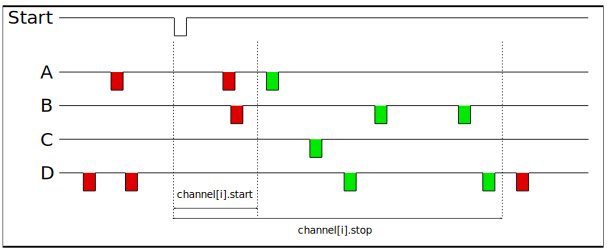
\includegraphics[width=0.7\textwidth]{figures/grouping.pdf}
        \caption{Acquired hits are merged to groups as explained in the text.\label{fig:grouping}}
    \end{center}
\end{figure*}


%
		\lstset{
	language=[Visual]C++,
	keywordstyle=\bfseries\sffamily\color[rgb]{0,0,1},
	identifierstyle=\sffamily,
	commentstyle=\color[rgb]{0.133,0.545,0.133},
	stringstyle=\sffamily\color[rgb]{0.627,0.126,0.941},
	showstringspaces=false,
	basicstyle=\small,
	numberstyle=\footnotesize,
	numbers=left,
	stepnumber=1,
	numbersep=10pt,
	tabsize=2,
	breaklines=true,
	prebreak = \raisebox{0ex}[0ex][0ex]{\ensuremath{\hookleftarrow}},
	breakatwhitespace=false,
	aboveskip={1.5\baselineskip},
	columns=fixed,
	upquote=true,
	extendedchars=true,
}

\section{Auto-Triggering Function Generator\label{cp:AutoTriggeringFunctionGenerator}}
Some applications require internal periodic or random triggering. The \deviceName\ function generator provides this functionality.\par

The delay between two trigger pulses of this trigger generator is the sum of two components: A fixed value M and a pseudo-random value with a range given by the exponent N. \par

The period is

\begin{align}
    T = 1 + M + [1...2^N]
\end{align}

clock cycles \ifxHPTDC{of the 150~MHz clock}{with a duration of $4~ns$ per cycle}.\par

The trigger can be used as a source for the TiGer unit (see Section \ref{cp:tiger}).


\section{Timing Generator (TiGer)\label{cp:tiger}}
Each digital LEMO-00 input can be used as an \ifxHPTDC{AC coupled}{LVCMOS} trigger output. 
The TiGer functionality can be configured independently for each connector. 
See Section \ref{cp:tigerblock} for a full description of the configuration options.
% 
\begin{figure*}[ht]
    \begin{center}
        \ifxHPTDC { 
            % this is an XCIrcuit drawing  convertex from postscript with 
            %ps2pdf.exe -dEPSCrop xhptdc8_trigger_matrix.ps
            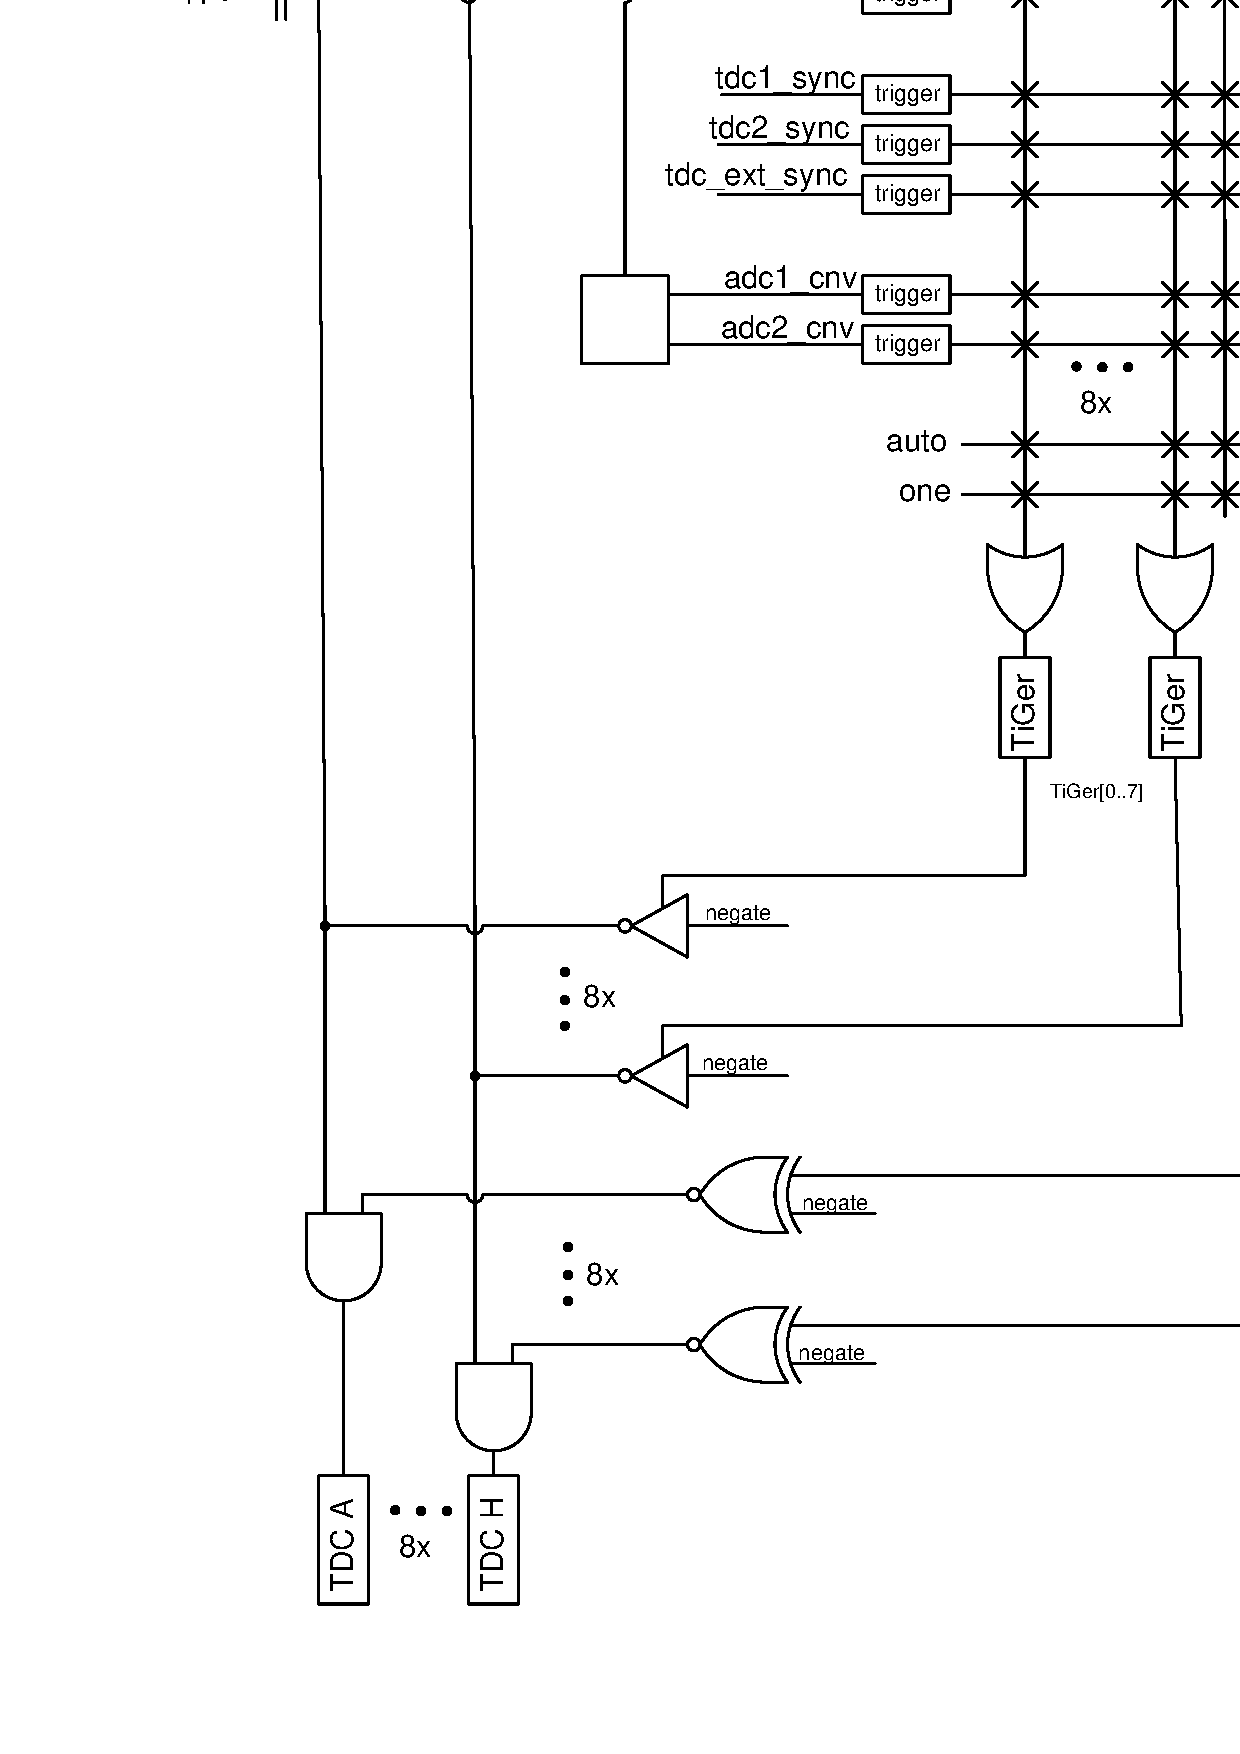
\includegraphics[width=0.6\textwidth]{xhptdc/figures/xhptdc8_trigger_matrix.pdf}
        }{
            \includegraphics[width=0.7\textwidth]{figures/xTDC4_tiger_matrix.pdf}
        }
        \caption{TiGer blocks can generate outputs that are also available on inputs.\label{fig:matrix}} 
    \end{center}
\end{figure*}
%

Figure \ref{fig:matrix} shows how the TiGer blocks are connected. They can be triggered by an OR of an arbitrary combination of inputs, 
including the auto-trigger \ifxHPTDC{and the ADC}{}. Each TiGer can drive its output to its corresponding LEMO connector. This turns the connector into an output. 

\ifxHPTDC{
	The TiGer outputs are AC coupled to the connector. They can be operated in one of the following modes:
	\paragraph*{\textsf{\PREFIX TIGER\tu OFF}} 
		No signal is output to the connetor. 
	\paragraph*{\textsf{\PREFIX TIGER\tu OUTPUT}} 
		In this mode the connector is output only. Pulses are unipolar with 2V amplitude. 
		Connected hardware must not drive any signals to connectors used as outputs, as doing so could damage both the \deviceName\ and the external hardware. 
		We recommend to only use short pulses to avoid undesirable baseline shift due to the AC coupling, but the device does not pose any restrictions on the duty cycle. 
		This mode can be used as a clock output with a frequency of $75/N$~MHz for integer $N$.
	\paragraph*{\textsf{\PREFIX TIGER\tu BIDI}} 
		In this mode the TiGer creates unipolar pulses with 1~V amplitude. The connector can still be used as an input. 
		Use short pulses to keep the probability of collision and the effect on the baseline low.	
	\paragraph*{\textsf{\PREFIX TIGER\tu BIPOLAR}} 
		In this mode the connector creates bipolar pulses with 1~V amplitude. The connector can still be used as an input. 
		Pulses have no effect on the baseline offset. 
		TiGer should be configured with $stop = start$ for minimum width bipolar pulses of $2 \times 6.\overline{6}~ns$. 
		The maximum bipolar pulse width is \textsf{XHPTDC8\tu TIGER\tu MAX\tu BIPOLAR\tu PULSE\tu LENGTH=15}.    
}{
	The TiGer is DC coupled to the connector. Connected hardware must not drive any signals to connectors used as outputs, 
	as doing so could damage both the \deviceName\  and the external hardware.
	Pulses that are short enough for the input AC coupling are available as input signals to the \deviceName. 
	This can be used to measure exact time differences between the generated output signals and input signals on other channels.
}

\ifxHPTDC{
	\newpage
	\subsection{Trigger Sources}
	\label{triggersources}
	Trigger sources for TiGer and gating blocks are configured by a bitmask. You can combine any number of trigger source with a bitwise or. 
	The block will be trigger when any of the select trigger input is active.

	\paragraph*{\textsf{\PREFIX TRIGGER\tu SOURCE\tu NONE}} \leavevmode \\
		Empty pattern that selects no trigger source.
	\paragraph*{\textsf{\PREFIX TRIGGER\tu SOURCE\tu A to \tu H}} \leavevmode \\
	 	TDC lemo inputs.   
	 \paragraph*{\textsf{\PREFIX TRIGGER\tu SOURCE\tu TDC1\tu SYNC}} \leavevmode \\
		Same as \textsf{\PREFIX TRIGGER\tu SOURCE\tu TDC2\tu SYNC}.\\*
		Clock signal with $150~MHz/1024\approx 146.5~kHz$. 
	\paragraph*{\textsf{\PREFIX TRIGGER\tu SOURCE\tu TDC\tu EXT\tu SYNC}} \leavevmode \\
		Clock signal with 125~kHz. 
	\paragraph*{\textsf{\PREFIX TRIGGER\tu SOURCE\tu AUTO}} \leavevmode \\
		Periodic or random trigger pulses from the auto-trigger block.
	\paragraph*{\textsf{\PREFIX TRIGGER\tu SOURCE\tu ADC1\tu CONV}} \leavevmode \\
		Same as \textsf{\PREFIX TRIGGER\tu SOURCE\tu ADC2\tu CONV}. When there is an ADC trigger pulse on the TRG connector, either of the two onboard ADCs is triggered in an unpredictable pattern. 
		If the TRG input shall be used as a trigger, the trigger sources must contain both \textsf{ADC1\tu CNV} and \textsf{ADC2\tu CNV}.
	\paragraph*{\textsf{\PREFIX TRIGGER\tu SOURCE\tu SOFTWARE}} \leavevmode \\
		Set for one clock cycle by a call to the driver function
		\textsf{\prefix software\tu trigger()}.
	\paragraph*{\textsf{\PREFIX TRIGGER\tu SOURCE\tu ONE}} \leavevmode \\
		Trigger that is active on every clock cycle.
	
	\ttinput{Tiger_Example.tex}	


	\subsection{Triggering the ADC with the TiGer}
		\label{adctiger}
		There is a ninth TiGer that is connected to the trigger input of the ADC. See section \ref{adc} for additional information on the ADC. 

		The ADC TiGer can be used with retrigger enabled to periodically sample ADC data. 
		The period should be no shorter than 300~ns or 45 TiGer clocks.

		The ADC TiGer can also be used to sample voltages at a time relative to one of the TDC inputs. In this case, 
		\textsf{stop} should be set to at least 45 to ensure that the sample period criterion is met even when pulses
		arrive in quick succession. A typical application would be to sample some slow control voltage once per start signal.

\newpage
	\section{Gating}
		Each TDC channel has a second, identical TiGer block that functions as a gate as shown in figure \ref{fig:matrix}. In driver configuration structure these are accessible as \textsf{gating\tu block[channel]}.
		Hits are recorded in a channel only while the output of the gating block is active.
		If the block is negated in the configuration, hits are only recorded while the gating block is inactive.
		
		This is a useful feature in setups where the trigger creates a lot of noise.
		A suitable configuration of the gating block can reduce the bandwidth and buffer usage significantly.
		Gating is performed before the L0 buffer. Grouping is performed in software after readout. 
		
	\section{Triggerable ADC}
		\label{adc}
		The \deviceName\ is equipped with a triggerable ADC. 
		Whenever there is a rising edge on the ADC trigger connector, 
		the voltage on the ADC input connector is sampled. 
		The result is inserted as a packet with timestamp and ADC value into the readout data stream.

		The ADC trigger also is connected to the output of a TiGer block. 
		This can be used to to trigger the ADC periodical or relative to one of the TDC input as described in section \ref{adctiger}

		The ADC triggers should not be closer than 300~ns apart.

		There are two interleaved ADCs  to ensure that there is always an ADC available even during readout. 
		This is exposed to the user both in the output data format and in the TiGer and Gating trigger sources.
		When using the ADC trigger as a trigger for Gating or TiGer both trigger sources shall be set to the same value.
		During readout, the user shall not distinguish between data from the two ADCs unless advanced calibration is 
		desired for the ADC data. In that case, the two ADCs should be treated separately.   

}{} 

	\chapter{Driver Programming API\label{cp:api}} 
		% also includes common/StructConfig.tex and common/InfoStructs.tex
		\ifxHPTDC{
    \newcommand{\device}{}
    \newcommand{\deviceindex}{\cronvar{int}{index}}
    \newcommand{\deviceconfig}{}
    \newcommand{\initparameters}{xhptdc8\tu manager\tu init\tu parameters}
}{
    \newcommand{\device}{\cronvar{\prefix device}{*device}}
    \newcommand{\deviceindex}{\device}
    \newcommand{\deviceconfig}{\deviceindex, }
    \newcommand{\initparameters}{\prefix init\tu parameters}
}

The API is a DLL with C linkage.\par

The functions provided by the driver are declared in
\texttt{\txh{TimeTagger4}{xTDC4}{xHPTDC8}\tu interface.h} 
which must be included by your source code.
You must tell your compiler to link with the file
\ifxHPTDC{%
    \texttt{xhptdc8\tu driver.lib} or the corresponding 64 bit version
    \texttt{xhptdc8\tu driver\tu 64.lib}.
}{%
    \textsf{xTDC4\tu driver\tu 64.lib}.}
When running your program the dynamic link library containing the actual
driver code must reside in the same directory as your executable or be in a
directory included in the PATH variable. For Linux, it is provided only as a
static library \texttt{libxtdc4\tu driver.a} 
The file for the DLL is called \texttt{xTDC4\tu driver\tu 64.dll}.

All these files are provided with the driver installer that can be downloaded
from the product website \href{https://www.cronologic.de}{www.cronologic.de}. 
By default, the installer will place the files into the directory 
\texttt{C:\filesep Program Files\filesep cronologic\filesep \deviceName\filesep driver}.
A coding example can be found on\\
\href{https://github.com/cronologic-de/xtdc_babel/tree/main/timetagger4_user_guide_example}{github.com/cronologic-de/xtdc\_babel}.

\ifxHPTDC{
    There exist an open-source community project that intends to provide some
    convenient extensions to the driver, code examples, and wrappers to make
    the driver usable with various programming languages like Python and
    LabView. The project is hosted at
    \url{https://github.com/cronologic-de/xhptdc8_babel}.
}{}

 
\section{Constants}
\ifxHPTDC{
    \begin{description}[style=nextline]
        \item[\crondef{XHPTDC8\tu MANAGER\tu DEVICES\tu MAX 6}]
        The maximum number of boards supported by the device manager.

        \item[\ttdef{TDC\tu CHANNEL\tu COUNT 8}]
        The number of TDC input channels.

        \item[\ttdef{GATE\tu COUNT 8}]
        The number of gating blocks. One for each TDC input.

        \item[\ttdef{TIGER\tu COUNT 9}]
        The number of timing generators. One for each TDC input and one for the
        ADC trigger.

        \item[\ttdef{TRIGGER\tu COUNT 16}]
        The number of potential trigger sources for the timing generators. One
        for each TDC input \ifxHPTDC{}{, one for the Start input} plus some
        specials.  See Section~\ref{structtrigger} for details.
}{ 
    \begin{description}[style=nextline]
        \item[\ttdef{TDC\tu CHANNEL\tu COUNT 4}]
        The number of TDC input channels.

        \item[\ttdef{TIGER\tu COUNT 5}]
        The number of timing generators. One for each TDC input and one for the
        start input.

        \item[\ttdef{TRIGGER\tu COUNT 16}]
        The number of potential trigger sources for the timing generators. One
        for each TDC input, one for the Start input plus some specials. See
        Section~\ref{cp:tigerblock} for details. 
}
    \item[\ttdef{OK 0}]
    Error codes are set by the API functions to this value if there has
    been no error. Other error codes can be found in
    \texttt{\txh{TimeTagger4}{xTDC4}{xHPTDC8}\tu interface.h}
\end{description}





\section{Driver Information}
Even if there is no board present the driver revision can be queried using
these functions.

\begin{description}[style=nextline]
    \item[\ttvar{int}{get\tu driver\tu revision()}]
    Returns the driver version, same format as \texttt{\prefix static\tu
    info.driver\tu revision}.  This function does not require \adeviceName\
    board to be present.

    \item[\ttvar{const char*}{get\tu driver\tu revision\tu str()}]
    Returns the driver version including SVN build revision as a string. 

    \item[\ttvar{int}{count\tu devices(}\cronvar{int}{*error\tu code},
    \cronvar{char}{**error\tu message)}\label{countdevices}]
    Returns the number of boards present in the system that are supported by
    this driver.  Pointers to an error code and message variable have to be
    provided. If {\ttfamily error\_code} does not equal
    {\ttfamily\ttdef{OK} = 0}, the error message will contain what went wrong.
    E.g., crono kernel was not properly installed. \par
\end{description}




\section{Initialization}
The card must be initialized first before reading data. Normally the process is
to get the default init parameters and change some values. E.g., choose one of
multiple cards by the index or use a larger buffer.
    

\begin{description}[style=nextline]
    \item[\ttvar{int}{get\tu default\tu init\tu
        parameters(}\cronvar{\initparameters}{*init)}]
    Sets up the standard parameters. Gets a set of default parameters for
    \texttt{\prefix init()}.  This must always be used to initialize the
    \texttt{\initparameters} structure before modifying it and passing it to
    \texttt{\prefix init}.

    \ifxHPTDC{
        \item[\ttvar{int}{init(}\cronvar{\initparameters}{*params})]
    }{
        \item[\cronvar{\prefix device}{\prefix
            init(}\cronvar{\initparameters}{*params}, \cronvar{int}{*error\tu
            code}, \cronvar{char}{**error\tu message)}]
    }
    Opens and initializes the \deviceName\ 
    \ifxHPTDC{boards in the system}{board with the given index}. \par
    \ifxHPTDC{
        If the return value does not equal {\ttfamily\ttdef{OK} = 0}
        the device initialization failed.
    }{
        \texttt{error\tu code} must point to an integer where the driver can 
        write the error code.\par
        \texttt{error\tu message} must point to a pointer to char.  The driver
        will allocate a buffer for zero-ter\-mi\-na\-ted error message and 
        store the address of the buffer in the location provided by the
        user.\par
    }
    The parameter \texttt{params} is a pointer to a structure of
    type \texttt{\initparameters} that must be completely initialized by
    \texttt{get\tu default\tu init\tu parameters()}.

    \item[\ttvar{int}{close(}\device )]
    Closes the devices, releasing all resources. 
\end{description}

%%%%%%%%%%%%%%%%% struct init_parameters

\subsection{Structure \initparameters}
\begin{description}[style=nextline]
    \item[\cronvar{int}{version}\txhinits{}{}{\PREFIX API\tu VERSION}]
    The version number. Must be set to \texttt{\PREFIX API\tu VERSION}.\par

    \ifxHPTDC{}{
        \item[\cronvar{int}{card\tu index}]
        The index in the list of \deviceName\ boards that should be
        initialized.\par
        There might be multiple boards in the system that are handled by this
        driver as reported by \texttt{\prefix count\tu devices}. This index
        selects one of them. Boards are enumerated depending on the PCIe slot.
        The lower the bus number and the lower the slot number the lower the
        card index.

        \item[\cronvar{int}{board\tu id}]
        The global index in all cronologic devices.\par
        This 8-bit number is filled into each packet created by the board and
        is useful if data streams of multiple boards will be merged. If only
        \deviceName\ cards are used this number can be set to the
        \texttt{card\tu index}.  If boards of different types that use a
        compatible data format are used in a system each board should get a
        unique id.  Can be changed with \texttt{int \prefix set\tu board\tu
        id\allowbreak(\prefix device *device, int board\tu id)}.}


    \item[\cronvar{uint64\tu t}{buffer\tu size\ifxHPTDC{}{[8]}}%
        \txhinits{}{}{XHPTDC\_DEFAULT\_BUFFER\_SIZE}%
        \txh{}{}{\normalfont\ttfamily\ // 0x1000000 (16 MB)}]
    The minimum size of the DMA buffer.\\
    If set to \texttt{0} the default size of 16\,MByte is used. 
    \ifxHPTDC{}{For the \deviceName\ only the first entry is used.}\par

    \ifxHPTDC{}{
        \item[\cronvar{int}{buffer\tu type}]
        The type of buffer. Must be set to \texttt{0}.
        \begin{description}
            \item[]  \ttdef{BUFFER\tu ALLOCATE   0}
            \item[]  \ttdef{BUFFER\tu USE\tu PHYSICAL   1}  // unsupported
        \end{description}

        \item[\cronvar{uint64\tu t}{buffer\tu address}]
        This is set by \texttt{\prefix init()} to the start address of the
        reserved memory.\par
        The buffers will be allocated with the sizes given above. Make sure
        that the memory is large enough.
    }

    \item[\cronvar{int}{variant}\txhinits{0}{0}{0}]
    Set to \texttt{0}. Can be used to activate future device variants such as
    different base frequencies.\par

    \item[\cronvar{int}{device\tu type}\txhinits{}{}{CRONO\_DEVICE\_XHPTDC8}]
    A constant for the different devices of cronologic
    \texttt{CRONO\tu DEVICE\tu *}.\par
    Initialized by \texttt{\prefix get\tu default\tu init\tu parameters()}.
    This value is identical to the PCI Device ID. Must be left unchanged.

    \begin{tabular}{ll}
        \crondef{CRONO\tu DEVICE\tu HPTDC}       & \ttfamily 0x1 \\
        \crondef{CRONO\tu DEVICE\tu NDIGO5G}     & \ttfamily 0x2 \\
        \crondef{CRONO\tu DEVICE\tu NDIGO250M}   & \ttfamily 0x4 \\
        \crondef{CRONO\tu DEVICE\tu xTDC4}       & \ttfamily 0x6 \\
        \crondef{CRONO\tu DEVICE\tu TIMETAGGER4} & \ttfamily 0x8 \\
        \crondef{CRONO\tu DEVICE\tu XHPTDC8}     & \ttfamily 0xC \\
        \crondef{CRONO\tu DEVICE\tu NDIGO6}      & \ttfamily 0xD \\
    \end{tabular}

    \item[\cronvar{int}{dma\tu read\tu delay}\txhinits{}{}{250}]
    The update delay of the write pointer after a packet has been sent over
    PCIe. Specified in multiples of \SI{16}{\nano\second}.  Should not be
    changed by the user.

    \ifxHPTDC{
        \item[\cronvar{crono\tu bool\tu t}{multiboard}\txhinits{}{}{false}]
        Set if multiple devices shall be synchronized. Also sets the clock
        source to external.

        \item[\cronvar{crono\tu bool\tu t}{use\tu ext\tu clock}%
            \txhinits{}{}{false}]
        If set use the external 10\,MHz reference on J2, otherwise the internal
        clock source is used.  When \texttt{multiboard} is set, this parameter
        is ignored and the external clock is used. 

        \item[\cronvar{crono\tu bool\tu t}{ignore\tu calibration}%
            \txhinits{}{}{false}]
        Leave at \texttt{false} to use device calibration data.

    }{
        \item[\cronvar{int}{use\tu ext\tu clock}]
        If set to \texttt{1}, use external 10\,MHz reference. If set to
        \texttt{0}, use internal reference.
    }
\end{description}

% info structures
\section{Status Information}
	

\subsection{Functions for Information Retrieval}
The driver provides functions to retrieve detailed information on the
board type, its configuration, settings, and state.  The information is
split according to its scope and the computational requirements to query
the information from the board.

\ifxHPTDC{
    The information is provided on a per board basis. The parameter
    \texttt{index} selects which board is queried.
}{}

\begin{description}[style=nextline]
    \item[\ttvar{int}{get\tu device\tu type}(\deviceindex)]
    Returns the type of the device as \texttt{CRONO\tu DEVICE\tu
    \txh{TIMETAGGER4}{XTDC4}{XHPTDC8}}.

    \item[\ttvar{const char*}{get\tu last\tu error\tu message(\deviceindex)}]
    Returns most recent error message.
    \ifxHPTDC{
        If index is negative the last error message from the \\
        \texttt{\prefix manager} is returned. Otherwise, the last error message
        of the selected board is returned.
    }{}

    \item[\ttvar{int}{get\tu fast\tu info(}\deviceindex, \cronvar{\prefix fast\tu info}{*info)}]
    Returns fast dynamic information.\par
    This call gets a structure that contains dynamic information that can be
    obtained within a few microseconds.

    \item[\ttvar{int}{get\tu param\tu info(}\deviceindex, \cronvar{\prefix param\tu info}{*info)}]
    Returns configuration changes.\par
    Gets a structure that contains information that changes indirectly due to
    configuration changes.


    \item[\ttvar{int}{get\tu static\tu info(}\deviceindex, \cronvar{\prefix static\tu info}{*info)}]
    Contains static information.\par
    Gets a structure that contains information about the board that does not
    change during run time.

    \item[\ttvar{int}{get\_pcie\_info(}\deviceindex, \cronvar{crono\_pcie\_info}{*pcie\_info)}]
    Read PCIe information.\par
    Gets a structure that contains information about the PCIe state, like
    correctable or uncorrectable errors.

    \item[\ttvar{int}{clear\_pcie\_errors(}\deviceindex, \cronvar{int}{flags)}]
    Clear PCIe errors.\par
    Only useful for PCIe debugging.
    \texttt{flags} is one of the following:
    \begin{tabular}{ll}
        \crondef{CRONO\_PCIE\_CORRECTABLE\_FLAG}   & \texttt{1}  \\*
        \crondef{CRONO\_PCIE\_UNCORRECTABLE\_FLAG} & \texttt{2}  \\*
    \end{tabular}


    \ifxHPTDC{
        \item[\ttvar{int}{get\tu temperature\tu info(}\deviceindex, \cronvar{\prefix temperature\tu info}{*info)}]
        Get temperature measurements from multiple sources on the board.

        \item[\ttvar{int}{get\tu clock\tu info(}\deviceindex, \cronvar{\prefix
            clock\tu info}{*info)}]
        Get information on clocking configuration and status.

        \item[\ttvar{const char*}{device\tu state\tu to \tu str(}\cronvar{int}{state)}]
        Convert the state value from \texttt{\prefix fast\tu info.state} into
        a human-readable string. 
    }{} 
\end{description}

%%%%%%%%%%%%%%%%% static info

\subsection{Structure \prefix static\tu info}

This structure contains information about the board that does not change during
run time. It is provided by the function
\texttt{\prefix get\tu static\tu info()}.

\begin{description}[style=nextline]
    \item[\cronvar{int}{size}]
    The number of bytes occupied by the structure.

    \item[\cronvar{int}{version}]
    A version number that is increased when the definition of the structure is
    changed. The increment can be larger than one to match driver version
    numbers or similar.

    \item[\cronvar{int}{board\tu id}]
    ID of the board.\par
    \ifxHPTDC{
        All \deviceName\ boards in the system are numbered in the order of
        their serial numbers starting at zero.  Channel A of a board has
        channel number $index \times 10$.
    }{}

    \item[\cronvar{int}{driver\tu revision}]
    Encoded version number for the driver.\par
    The lower three bytes contain a triple-level hierarchy of version numbers,
    e.g., \texttt{0x010103} encodes version 1.1.3.\par
    The version adheres to the Semantic Versioning scheme as defined at
    \href{https://semver.org}{https://semver.org}. A change in the first digit
    generally requires a recompilation of user applications.  Changes in the
    second digit denote significant improvements or changes that don't break
    compatibility and the third digit increments with minor bug fixes and
    similar updates that do not affect the API.

    \item[\cronvar{int}{driver\tu build\tu revision}]
    Build number of the driver according to cronologic's internal versioning
    system.

    \item[\cronvar{int}{firmware\tu revision}]
    Revision number of the FPGA configuration.

    \item[\cronvar{int}{board\tu revision}]
    Board revision number.\par
    The board revision number can be read from a register. It is a four-bit
    number that changes when the schematic of the board is changed. This should
    match the revision number printed on the board.

    \item[\cronvar{int}{board\tu configuration}]
    Describes the schematic configuration of the board.\par
    The same board schematic can be populated in multiple variants. This is an
    8-bit code that can be read from a register.

    \item[\cronvar{int}{subversion\tu revision}]
    Subversion revision ID of the FPGA configuration source code.

    \txh{
        \item[\cronvar{int}{chip\tu id}]
        Reserved.
    }{
        \item[\cronvar{int}{chip\tu id}]
        16 bit factory ID of the TDC chip.
    }{
        \item[\cronvar{int}{chip\tu id[2]}]
        16 bit factory ID for each of the TDC chips.
    }

    \item[\cronvar{int}{board\tu serial}]
    Serial number.\par
    Year and running number are concatenated in 8.24 format. The number is
    identical to the one printed on the silvery sticker on the board.

    \item[\protect{\parbox[b]{0.8\linewidth}{
        \cronvar{\uint}{flash\tu serial\tu high}\\
        \cronvar{\uint}{flash\tu serial\tu low}}}]
    64-bit manufacturer serial number of the flash chip

    \item[\cronvar{crono\tu bool\tu t}{flash\tu valid}]
    If not \texttt{0}, the driver found valid calibration data in the flash on
    the board and is using it. This value is not applicable for the
    \deviceName.

    \item[\cronvar{char}{calibration\tu date[20]}]
    DIN EN ISO 8601 string YYYY-MM-DD HH:MM of the time when the card
    was calibrated.

    \ifxHPTDC{}{
        \item[\cronvar{char}{bitstream\tu date[20]}]
        DIN EN ISO 8601 string YYYY-MM-DD HH:MM of the time when the bitstream
        on the card was created.
    }

    \txh{
        \item[\cronvar{double}{delay\tu bin\tu size}]
        Bin size of delay in picoseconds. The increment of the
        \texttt{delay\tu config.delay} field for the \deviceName.

        \item[\cronvar{double}{auto\tu trigger\tu ref\tu clock}]
        Auto trigger clock frequency. The clock frequency of the auto trigger
        in Hertz used for calculating the \texttt{auto\tu trigger\tu period}.

        \item[\cronvar{uint32\tu t}{rollover\tu period}]
        The number of bins in a rollover period. This is a power of 2 (the
        maximum value of a hit timestamp is this value minus 1)
    }{}{}
\end{description}

%%%%%%%%%%%%%%%%%%%%%%%% param info
\subsection{Structure \prefix param\tu info}
This structure contains configuration changes provided by \texttt{\prefix
get\tu param\tu info()}.

\begin{description}[style=nextline]
    \item[\cronvar{int}{size}]
    The number of bytes occupied by the structure.

    \item[\cronvar{int}{version}]
    A version number that is increased when the definition of the structure is
    changed. The increment can be larger than one to match driver version
    numbers or similar.

    \item[\cronvar{double}{binsize}]
    Bin size (in \si{\pico\second}) of the measured TDC data.

    \ifxHPTDC{}{ %board ID is found in the static_info structure for .
        \item[\cronvar{int}{board\tu id}]
        Board ID.\par
        The board uses this ID to identify itself in the output data stream.
        The ID takes values between \texttt{0} and \texttt{255}.
    }

    \item[\cronvar{int}{channels}]
    Number of TDC channels of the board.\par
    Fixed at \texttt{\ifxHPTDC{8}{4}}.

    \item[\cronvar{int}{channel\tu mask}]
    Bit assignment of each enabled input channel.\par
    Bit $\texttt{0} \leq n < \texttt{\ifxHPTDC{8}{4}}$ is set if channel $n$ is
    enabled.

    \item[\cronvar{int64\tu t}{total\tu buffer}]
    The total amount of DMA buffer in bytes.

    \ifxHPTDC{}{
        \item[\cronvar{double}{packet\tu binsize}]
        \itett{ %tt4
            For the \deviceName\, the packet binsize is equal to the binsize
            and depends on the generation of the card. Gen\,1 boards have a
            packet binsize of \SI{500}{\pico\second}, while Gen\,2 boards have
            \SI{100}{\pico\second}.
        }{ %xtdc4
            For \deviceName\, this is \SI{1666.6}{\pico\second}
        }
    }

    \ifxHPTDC{}{
        \item[\cronvar{double}{quantisation}]
        \itett{ %tt4
            Quantisation or measurement resolution. Depending on the board
            variant this ranges from \SIrange{100}{1000}{\pico\second}.\par
            \begin{tabular} {|l|l|l|l|l|l|l}
            \hline
            --1G & --2G & --1.25G & --2.5G & --5G & --10G \\
            \hline
            1000 ps & 500 ps & 800 ps & 400 ps & 200 ps & 100 ps\\
            \hline
            \end{tabular}

            This means, that for --1.25G the lower 3 bits in the timestamps are
            zero.
        }{ %xtdc4
            Quantisation or measurement resolution. For the \deviceName\, this
            is \SI{13.0208}{\pico\second}
        }
    }
\end{description}

%%%%%%%%%%%%%%%%%%%%%%%%%% fast info

\subsection{Structure \prefix fast\tu info} \label{structfastinfo}
\begin{description}[style=nextline]
    \item[\cronvar{int}{size}]
    The number of bytes occupied by the structure. 

    \item[\cronvar{int}{version}]
    A version number that is increased when the definition of the structure is
    changed.  The increment can be larger than one to match driver version
    numbers or similar.

    \ifxHPTDC{} {
        \item[\cronvar{int}{tdc\tu rpm}]
        Speed of the TDC fan in rounds per minute. Reports \texttt{0} if no fan
        is present.
    }

    \item[\cronvar{int}{fpga\tu rpm}]
    Speed of the FPGA fan in rounds per minute. Reports \texttt{0} if no fan is
    present.

    \item[\cronvar{int}{alerts}]
    Alert bits from the temperature sensor and the system monitor.
    \itett{
        The TimeTagger4 does not implement any temperature alerts.
    }{
        Bit 0 is set if the TDC temperature exceeds \SI{140}{\degreeCelsius}. 
        In this case the TDC did shut down and the device needs to be
        reinitialized. 
    }

    \item[\cronvar{int}{pcie\tu pwr\tu mgmt}]
    Always \texttt{0}.

    \item[\cronvar{int}{pcie\tu link\tu width}]
    Number of PCIe lanes the card uses. Should always be \texttt{10} for the
    \deviceName.

    \item[\cronvar{int}{pcie\tu max\tu payload}]
    Maximum size in bytes for one PCIe transaction. Depends on system
    configuration.

    \ifxHPTDC{
    \item[\cronvar{int}{state}]
    Current state of the \deviceName. 

    \begin{tabular}{lc}
        \cronvar{const static int}{\PREFIX DEVICE\tu STATE\tu CREATED} & \texttt{0}  \\*
        \cronvar{const static int}{\PREFIX DEVICE\tu STATE\tu INITIALIZED} & \texttt{1}  \\*
        \cronvar{const static int}{\PREFIX DEVICE\tu STATE\tu CONFIGURED} & \texttt{2}  \\*
        \cronvar{const static int}{\PREFIX DEVICE\tu STATE\tu CAPTURING} & \texttt{3}  \\*
        \cronvar{const static int}{\PREFIX DEVICE\tu STATE\tu PAUSED} & \texttt{4}  \\*
        \cronvar{const static int}{\PREFIX DEVICE\tu STATE\tu CLOSED} & \texttt{5}  \\*
    \end{tabular}
    }{}
\end{description}


%%%%%%%%%%%%%%%%%%%%%%%%%%%%%% PCIe Info
\subsection{Structure crono\_pcie\_info}
\begin{description}[style=nextline]
    \item[\cronvar{uint32\_t}{pwr\_mgmt}]
    Organizes power supply of PCIe lanes.

    \item[\cronvar{uint32\_t}{link\_width}]
    Number of PCIe lanes that the card uses.\par

    \item[\cronvar{uint32\_t}{max\_payload}]
    Maximum size in bytes for one PCIe transaction.\par
    Depends on the system configuration.

    \item[\cronvar{uint32\_t}{link\_speed}]
    Data rate of the PCIe card.\par
    Depends on the system configuration.

    \item[\cronvar{uint32\_t}{error\_status\_supported}]
    Different from 0 if the PCIe error status is supported for this device.

    \item[\cronvar{uint32\_t}{correctable\_error\_status}]
    Correctable error status flags, directly from the PCIe config register.\par
    Useful for debugging PCIe problems.

    \begin{tabular}{ll}
        \crondef{CRONO\_PCIE\_RX\_ERROR} & \texttt{1 << 0}  \\*
        \crondef{CRONO\_PCIE\_BAD\_TLP} & \texttt{1 << 6}  \\*
        \crondef{CRONO\_PCIE\_BAD\_DLLP} & \texttt{1 << 7}  \\*
        \crondef{CRONO\_PCIE\_REPLAY\_NUM\_ROLLOVER} & \texttt{1 << 8}  \\*
        \crondef{CRONO\_PCIE\_REPLAY\_TIMER\_TIMEOUT} & \texttt{1 << 12}  \\*
        \crondef{CRONO\_PCIE\_ADVISORY\_NON\_FATAL} & \texttt{1 << 13}  \\*
        \crondef{CRONO\_PCIE\_CORRECTED\_INTERNAL\_ERROR} & \texttt{1 << 14}  \\*
        \crondef{CRONO\_PCIE\_HEADER\_LOG\_OVERFLOW} & \texttt{1 << 15}  \\*
    \end{tabular}

    \item[\cronvar{uint32\_t}{correctable\_error\_status}]
    Uncorrectable error status flags, directly from the PCIe config register.

    Useful for debugging PCIe problems.

    \begin{tabular}{ll}
        \crondef{CRONO\_PCIE\_UNC\_UNDEFINED}                      & \texttt{1 << 0}  \\*
        \crondef{CRONO\_PCIE\_UNC\_DATA\_LINK\_PROTOCOL\_ERROR}    & \texttt{1 << 4}  \\*
        \crondef{CRONO\_PCIE\_UNC\_SURPRISE\_DOWN\_ERROR}          & \texttt{1 << 5}  \\*
        \crondef{CRONO\_PCIE\_UNC\_POISONED\_TLP}                  & \texttt{1 << 12}  \\*
        \crondef{CRONO\_PCIE\_UNC\_FLOW\_CONTROL\_PROTOCOL\_ERROR} & \texttt{1 << 13}  \\*
        \crondef{CRONO\_PCIE\_UNC\_COMPLETION\_TIMEOUT}            & \texttt{1 << 14}  \\*
        \crondef{CRONO\_PCIE\_UNC\_COMPLETER\_ABORT}               & \texttt{1 << 15}  \\*
        \crondef{CRONO\_PCIE\_UNC\_UNEXPECTED\_COMPLETION}         & \texttt{1 << 16}  \\*
        \crondef{CRONO\_PCIE\_UNC\_RECEIVER\_OVERFLOW\_ERROR}      & \texttt{1 << 17}  \\*
        \crondef{CRONO\_PCIE\_UNC\_MALFORMED\_TLP}                 & \texttt{1 << 18}  \\*
        \crondef{CRONO\_PCIE\_UNC\_ECRC\_ERROR}                    & \texttt{1 << 19}  \\*
        \crondef{CRONO\_PCIE\_UNC\_UNSUPPROTED\_REQUEST\_ERROR}    & \texttt{1 << 20}  \\*
    \end{tabular}

\end{description}


%%%%%%%%%%%%%%%%%%%%%%% temperature info

\ifxHPTDC{
    \subsection{Structure \prefix temperature\tu info}
    This structure provides the values of temperature measurements of
    various chips on the board.

    \begin{description}[style=nextline]
        \item[\cronvar{int}{size}]
        The number of bytes occupied by the structure.

        \item[\cronvar{int}{version}]
        A version number that is increased when the definition of the
        structure is changed. The increment can be larger than one to match
        driver version numbers or similar.

        \item[\cronvar{float}{tdc[2]}]
        Temperature for each of the TDC chips in \si{\degreeCelsius}.
    \end{description}

    %%%%%%%%%%%%%%%%%%%%% clock info

    \subsection{Structure \prefix clock\tu info}
    This structure provides information about the clock network of the
    device. 

    \begin{description}[style=nextline]
        \item[\cronvar{int}{size}]
        The number of bytes occupied by the structure.

        \item[\cronvar{int}{version}]
        A version number that is increased when the definition of the structure
        is changed. The increment can be larger than one to match driver
        version numbers or similar.\par

        \item[\cronvar{crono\tu bool\tu t}{cdce\tu locked}]
        Set if the jitter cleaning PLL clock synthesizer achieved lock.

        \item[\cronvar{int}{cdce\tu version}]
        Version information from the CDCE62005 clock synthesizer.
        
        \item[\cronvar{crono\tu bool\tu t}{use\tu ext\tu clock}]
        Source for the clock synthesizer is usually the 10~MHz onboard
        oscillator. During initialization, alternatively an external clock
        on J2 can be selected.  When multiple boards are synchronized all board
        use a common external clock. See section \ref{multiboard} for details.
    
        \item[\cronvar{crono\tu bool\tu t}{fpga\tu locked}]
        Set if the FPGA data-path PLL achieved lock.
    \end{description}
}{}



\section{Configuration}
\ifxHPTDC{
    All \deviceName\ boards in the system are configured by a single
    configuration structure which in turn contains sub structures that
    configure the individual boards.
}{
    The device is configured with a configuration structure.
}
The user should first obtain a structure that contains the default settings of
the device read from an on-board ROM, then modify the structure as needed for
the user application and use the result to configure the device.\par

\begin{description}[style=nextline]
    \item[\ttvar{int}{configure(}\deviceconfig\cronvar{\prefix\ifxHPTDC{manager\tu }{}configuration}{*config)}]
    Configures the \texttt{\prefix manager}.

    \item[\protect{\parbox[b]{1.0\linewidth}{
        \ttvar{int}{get\tu current\tu configuration(}\deviceconfig
        \ifxHPTDC{}{\hspace*{\labelwidth+\itemsep}}\cronvar{
            \prefix\ifxHPTDC{manager\tu }{}configuration}{\textbf{*config})}}}]
    Gets current configuration. Copies the current configuration to the
    specified config pointer.

    \item[\protect{\parbox[b]{1.0\linewidth}{
        \ttvar{int}{get\tu default\tu configuration(}\deviceconfig
        \ifxHPTDC{}{\hspace*{\labelwidth+\itemsep}}\cronvar{
            \prefix \ifxHPTDC{manager\tu}{}configuration}{\textbf{*config})}}}]
    Gets default configuration. Copies the default configuration to the
    specified config pointer.
\end{description}

\ifxHPTDC{
    \subsection{YAML config files}
    \label{yaml}
    There exist a community maintained utility library for the \deviceName\
    that contains a convenience function that can modify configuration
    structures from a YAML config string. This can significantly shorten code
    required to setup the TDC. \par
    See \href{https://github.com/cronologic-de/xhptdc8_babel/tree/main/util}{
        github.com/cronologic-de/xhptdc8\tu babel/tree/main/util} for details.  
}{} 

%%%%%%%%%%%%%%%%% configuration structure mostly shared between devices
\subsection{Structure \prefix configuration}

			This is the structure containing the configuration information. It is used in conjunction with \textsf{\prefix get\tu default\tu configuration()}, \textsf{\prefix get\tu current\tu configuration()} and \textsf{\prefix configure()}.\par

			It uses the substructures \textsf{\prefix tiger\tu block} and \textsf{\prefix trigger}.\par

			\cronvar{int}{size}\\
			The number of bytes occupied by the structure.\par

			\cronvar{int}{version}\\
			A version number that is increased when the definition of the structure is changed. The increment can be larger than one to match driver version numbers or similar. Currently only version 0 is defined.\par

			\cronvar{int}{tdc\tu mode}\\
			TDC mode. Can be grouped or continuous. \\
			\ifxHPTDC{
				This defines whether grouping is used by the \textsf{Read()} method. Defaults to \textsf{\PREFIX TDC\tu MODE\tu CONTINOUS} 	
			}{
				Currently only \textsf{\PREFIX TDC\tu MODE\tu GROUPED} is supported. 
				This is set per default by \textsf{\prefix get\tu current\tu configuration()} and should be left unchanged.\par
			}
			\cronvar{crono\tu bool\tu t}{start\tu rising} 
			\itett{
				Not applicable for the \deviceName.
			}{
				Selects whether the rising or falling edge of the start signal is used to start a group.
			}\par

			\cronvar{double}{dc\tu offset[\PREFIX CHANNEL\tu COUNT + 1]}\\
			Set the threshold voltage for the input channels S, A - D (see figure \ref{fig:dcoffset1}).
			\begin{itemize}
				\item dc\tu offset[0] : threshold for channel Start
				\item dc\tu offset[1 - 4] : threshold for channels A \ldots D
			\end{itemize}
			Supported range is -1.32V to +1.18V. This should be close to 50\% of the height of the input pulse. Examples for various signaling standards are defined as follows\par
			\begin{tabular}{ll}
				\crondef{DC\tu OFFSET\tu P\tu NIM} & +0.35\\
				\crondef{DC\tu OFFSET\tu P\tu CMOS} & +1.18\\
				\crondef{DC\tu OFFSET\tu P\tu LVCMOS\tu 33} & +1.18\\
				\crondef{DC\tu OFFSET\tu P\tu LVCMOS\tu 25} & +1.18\\
				\crondef{DC\tu OFFSET\tu P\tu LVCMOS\tu 18} & +0.90\\
				\crondef{DC\tu OFFSET\tu P\tu TTL} & +1.18\\
				\crondef{DC\tu OFFSET\tu P\tu LVTTL\tu 33} & +1.18\\
				\crondef{DC\tu OFFSET\tu P\tu LVTTL\tu 25} & +1.18\\
				\crondef{DC\tu OFFSET\tu P\tu SSTL\tu 3} & +1.18\\
				\crondef{DC\tu OFFSET\tu P\tu SSTL\tu 2} & +1.18\\
				\crondef{DC\tu OFFSET\tu N\tu NIM} & -0.35\\
				\crondef{DC\tu OFFSET\tu N\tu CMOS} & -1.32\\
				\crondef{DC\tu OFFSET\tu N\tu LVCMOS\tu 33} & -1.32\\
				\crondef{DC\tu OFFSET\tu N\tu LVCMOS\tu 25} & -1.25\\
				\crondef{DC\tu OFFSET\tu N\tu LVCMOS\tu 18} & -0.90\\
				\crondef{DC\tu OFFSET\tu N\tu TTL} & -1.32\\
				\crondef{DC\tu OFFSET\tu N\tu LVTTL\tu 33} & -1.32\\
				\crondef{DC\tu OFFSET\tu N\tu LVTTL\tu 25} & -1.25\\
				\crondef{DC\tu OFFSET\tu N\tu SSTL\tu 3} & -1.32\\
				\crondef{DC\tu OFFSET\tu N\tu SSTL\tu 2} & -1.25\\
			\end{tabular}\par
			 \noindent The inputs are AC coupled. Thus, the absolute voltage is not important for pulse inputs. It is the relative pulse amplitude that causes the input circuits to switch. \textit{dc\tu offset} must be set to the relative switching voltage for the input standard in use. If the pulses are negative, a negative switching threshold must be set and vice versa.
			\begin{figure}
				\begin{center}
					\ifxHPTDC{
						\includegraphics[width=0.3\textwidth]{xhptdc/figures/InputCircuit.pdf}
					}{
						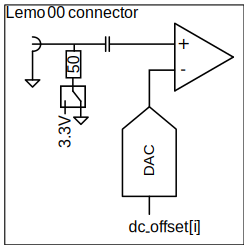
\includegraphics[width=0.3\textwidth]{figures/InputCircuit.pdf}
					}
					\caption{Input circuit for each of the input channels. \label{fig:dcoffset1}}
				\end{center} 
			\end{figure}
%%			\begin{figure}
%%				\begin{center}
%%					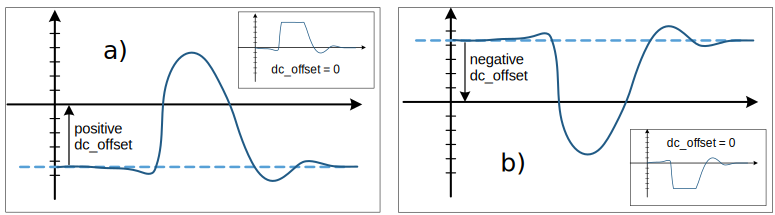
\includegraphics[width=\textwidth]{figures/dc_offset.pdf}
%%%					\caption{\textit{dc\tu offset} is used to shift the signal on each input channel such that the noise margin relative to the switching threshold is maximized.
%%					Insets of figure a) and b) show the base line of the signal with $\mathrm{\textit{dc\tu offset}}~=~0$ close to the switching threshold of the input buffer. Figure a) shows the positive pulse with $\mathrm{\textit{dc\tu offset}}~>~0$ and figure b) shows the negative pulse with $\mathrm{\textit{dc\tu offset}}~<~0$.\label{fig:dcoffset2}}
%%				\end{center}
%%			\end{figure}

			\ttvar{\prefix trigger}{trigger[\PREFIX TRIGGER\tu COUNT]}\\
			Configuration the polarity of the external trigger sources.
			These are used as inputs for the TiGer blocks and as inputs to the time measurement unit.\par

			\ttvar{\prefix tiger\tu block}{tiger\tu block[\PREFIX TIGER\tu COUNT]}
			Configuration of the timing generator (TiGer).

			\ttvar{\prefix channel}{channel[\PREFIX CHANNEL\tu COUNT]}\\
				Configure the TDC channels.

			\ttvar{\prefix low-res\tu channel}{low-res\tu channel[\PREFIX LOWRES\tu CHANNEL\tu COUNT]}\\
			\itett{
				Not applicable for \deviceName. 
			}{
				Only applicable to the xTDC4-Sciex. Configures the additional digital low-res inputs.
			}\par

			\cronvar{int}{auto\tu trigger\tu period}\\
			\cronvar{int}{auto\tu trigger\tu random\tu exponent}\\
			Create a trigger either periodically or randomly. There are two parameters $M = \text{trigger\tu period}$ and $N = \text{random\tu exponent}$ that result in a distance between triggers of $T$ clock cycles.

			\begin{align}
				T &= 1 + M + [1...2^N]\\
				&0 \leq M < 2^{32}\\
				&0 \leq N < 32
			\end{align}

			\noindent There is no enable or reset as the usage of this trigger can be configured in the TiGer block channel source field.\par

			\subsection{Structure \prefix trigger}
			\label{structtrigger}
			\cronvar{crono\tu bool\tu t}{falling}\\
			\cronvar{crono\tu bool\tu t}{rising}\\
			Select for which edges a trigger event is created inside the FPGA.
			\itett{
				The \deviceName can output measurements for one or both edges of input signals. 
			}{
				The \deviceName can output measurements with a reduced bin size of $5/6~ns = 833,\overline{3}~ps$ for one or both edges of input signals. 
				See section \ref{difficulthits} for more information on hits with varying resolution.
				Use \textsf{xtdc4\tu channel.rising} on page \pageref{structchannel} to select which edge is measured with full resolution.
				The edge that is selected for full resolution measurement must also be enabled for low resolution measurement.
			}\par

%%%%% tiger_block			

			\subsection{Structure \prefix tiger\tu block\label{cp:tigerblock}}

			\ifxHPTDC{
				\cronvar{int}{mode}\\
				Enables the desired mode of operation for the tiger.

				\begin{tabular}{lrl}
					\ttdef{TIGER \tu OFF} & 0 & no operation \\
					\ttdef{TIGER \tu OUTPUT} & 1 & output is driven with 2V amplitude. There must be no input connected \\
					\ttdef{TIGER \tu BIDI} & 2 & output is driven with 1V amplitude. Pulse rate should be low. \\
					\ttdef{TIGER \tu BIDI} & 2 & output is driven wuth 1V bidirectional pulses. $start = stop -1$\\
				\end{tabular}

				Gating blocks interpret any value that is not \ttdef{TIGER \tu OFF} as enable.	
			}{
				\cronvar{crono\tu bool\tu t}{enable}\\
				Activates the timing generator (TiGer).\par
			}
	
			\cronvar{crono\tu bool\tu t}{negate}\\
			Inverts output polarity. Default is set to false.
			\ifxHPTDC{For gating blocks, a value of false blocks inputs between start and stop, a value of true blocks outputs outside that interval.}{}\par
	
			\cronvar{crono\tu bool\tu t}{retrigger}\\
			Enables retrigger setting.\\
			If enabled the timer is reset to the value of the \textsf{start} parameter, whenever the input signal is set while waiting to reach the \textsf{stop} time.\par
	
			\cronvar{crono\tu bool\tu t}{extend}\\
			Not implemented.
	
			\ifxHPTDC{}{
				\cronvar{crono\tu bool\tu t}{enable\tu lemo\tu output}\\
				Enables the LEMO output. Drive the TiGer Signal to the corresponding Lemo connector as an output. 
				This is DC coupled, so make sure that you do not any devices connected as inputs.
				Pulses created by the TiGer are visible at the \deviceName inputs and can be measured again to get the exact timing.  
			}

			\cronvar{int}{start}\\
			\cronvar{int}{stop}\\
			\itett{
				In multiples of $4~ns$.
			}{
				In multiples of $20/3 = 6,\overline{6}~ns$
			}
			The time during which the TiGer output is set, relative to the trigger input. The parameters \textsf{start} and \textsf{stop} must fulfill the following conditions:
			\[ 0 <= start <= stop <= 2^{16}-1 \]
			If retriggering is enabled, the timer is reset to the value of the start parameter whenever the input signal is set while waiting for the stop time. \par
			
	
			\cronvar{int}{sources}\\
			A bit mask with a bit set for all trigger sources that can trigger this TiGer block. 
			Default is \textsf{\PREFIX TRIGGER\tu SOURCE\tu S}.\par
	
			\begin{tabular}{lc}
					 \ttdef{TRIGGER\tu SOURCE\tu S} & 0x00000001\\
					 \ttdef{TRIGGER\tu SOURCE\tu A} & 0x00000002\\
					 \ttdef{TRIGGER\tu SOURCE\tu B} & 0x00000004\\
					 \ttdef{TRIGGER\tu SOURCE\tu C} & 0x00000008\\
					 \ttdef{TRIGGER\tu SOURCE\tu D} & 0x00000010\\
					% \ttdef{TRIGGER\tu SOURCE\tu S1} & 0x00000020\\
					% \ttdef{TRIGGER\tu SOURCE\tu S2} & 0x00000040\\
					% \ttdef{TRIGGER\tu SOURCE\tu GATE} & 0x00000080\\
					 \ttdef{TRIGGER\tu SOURCE\tu AUTO} & 0x00004000\\
					 \ttdef{TRIGGER\tu SOURCE\tu ONE} & 0x00008000
				\end{tabular} 
	
			\subsection{Structure \prefix channel}
				\label{structchannel}
				Contains TDC channel settings.\par
	
				\cronvar{crono\tu bool\tu t}{enabled}\\
				Enable TDC channel.\par
	
				\cronvar{crono\tu bool\tu t}{rising}\\
				\itett{
					Not applicable for \deviceName.
				}{
					Select which edge of the signal is used for full resolution measurements. 
					\textsf{xtdc4\tu trigger.rising} and \textsf{xtdc4\tu trigger.falling} described on page \pageref{structtrigger} are used 
					to select which edges are recorded for low resolution measurement. 
					The edge that is selected for full resolution measurement must also be enabled for low resolution measurement.
					See section \ref{difficulthits} for more information on hits with varying resolution.
				}\par

				\itett{}{ % onyl for xTDC4
					\cronvar{crono\tu bool\tu t}{cc\tu enable}\\
					Enable carry chain TDC. This is set to \emph{true} by default and should be left unchanged. \par
	
					\cronvar{crono\tu bool\tu t}{cc\tu same\tu edge}\\
					Sets whether the carry chain TDC records the same or opposite edge as the TDC chip. 
					If the same edge is selected, that carry chain TDC acts  as a backup if the chip misses hits due to FIFO overflows or short input pulses.
					If opposite edges are selected, both edges of a pulse can be measured with reasonable resolution. See section \ref{difficulthits} for more information.\par
	
					\cronvar{crono\tu bool\tu t}{ths788\tu disable}\\
					Disable full resolution timestamps. This is set to \emph{false} by default and should be left unchanged.\par
				}
	
				\cronvar{int}{start}\\
				\cronvar{int}{stop}\\
				Veto function for grouping of hits into packets in multiples of the binsize. Only hits between start and stop are read out.
				The parameters must adhere to the following relations:
				\[
					0 <= start <= stop < 2^{ \itett{31}{30}}
				\]
	
	


%%%%%%%%%%%%%%

\ifxHPTDC{
    \section{User Data Storage}
    There is a 64~kByte flash memory on each board that users can utilize to
    store any type of data.  A typical use case would be calibration data for
    the \deviceName\ or the detectors that the device is connected to.  Also
    serial numbers of instruments built with the \deviceName\ can be stored
    here. Write operations always erase the whole memory block.\par

    \begin{description}[style=nextline]
        \item[\ttdef{USER\tu FLASH\tu SIZE 0x10000}]
        The size of the flash memory in bytes.\\

        \item[\protect{\parbox[b]{1.0\linewidth}{
            \ttvar{int}{read\tu user\tu flash(\cronvar{int}{index}, \cronvar{\uchar *}{flash\tu data}, \cronvar{\uint}{size})}\\
            \ttvar{int}{write\tu user\tu flash(\cronvar{int}{index}, \cronvar{\uchar *}{flash\tu data}, \cronvar{\uint}{size})}
        }}]
        Read from or write to the user flash of a board identified by
        \texttt{index}.  \texttt{flash\tu data} must point to a buffer
        allocated by the user.  \texttt{size} must specify the size of that
        buffer in bytes.  We recommend to always allocate a buffer of the size
        of the flash memory given by \texttt{\PREFIX FLASH\tu SIZE} to clarify
        that always the full buffer is overwritten.
    \end{description}
}{} 


    
  
		  
	\chapter{Run Time Control\label{cp:readout}}  % and packet format
		\ifxHPTDC{
				%%%%%%%%%%%%%%%%% run time control
	\section{Controlling the State of the Driver}
		\ttvar{int}{start\tu capture(}\device)\\
		Start data acquisition.\par

		\ttvar{int}{pause\tu capture(}\device)\\
		Pause a started data acquisition. 
		Pause and continue have less overhead than start and stop but don't allow for a configuration change.\par

		\ttvar{int}{continue\tu capture(}\device)\\
		Call this to resume data acquisition after a call to \textsf{\prefix pause\tu capture()}.
		Pause and continue have less overhead than start and stop but don't allow for a configuration change.\par

		\ttvar{int}{stop\tu capture(}\device)\\
		Stop data acquisition.\par

		\ttvar{int}{start\tu tiger(}\device, \cronvar{int}{index})\\
		\ttvar{int}{stop\tu tiger(}\device, \cronvar{int}{index})\\
		Start and stop the timing generator of an individual board. 
		This can be done independently of the state of the data acquisition.\par	


\section{Readout}

\ttvar{int}{read\tu hits(}\device,  \cronvar{TDCHit}{*hit\tu buf,} \cronvar{size\tu t}{size} )\\
Read a multitude of hits into a buffer provided by the user. Returns the number of read hits.\\
If grouping is enabled a single group is read. 
If the group is to large for the buffer the remaining hits of the group are discarded.\\*
If grouping is disabled, all availabe data is read up to the size of the buffer. \\
The method always returns immediately. If no hits are read it of is beneficial to call \textsf{sleep()} 
or yield the CPU to another process instead of trying again immediately.\\
Make sure to set \textsf{size} to the number of elemenst that fit into the buffer.\\*





		}{
			% NOTE: xHPTDC has a seperate file describing the readout

%%%%%%%%%%%%%%%%% run time control
\section{Run Time Control}

Once the devices are configured the following functions can be used to control
the behaviour of the devices.  All of these functions return quickly with very
little overhead, but they are not guaranteed to be thread safe.

\begin{description}[style=nextline]
    \item[\ttvar{int}{start\tu capture(}\device)]
    Start data acquisition.\par

    \item[\ttvar{int}{pause\tu capture(}\device)]
    Pause a started data acquisition. \par
    \texttt{pause} and \texttt{continue} have less overhead than start and
    stop but don't allow for a configuration change.

    \item[\ttvar{int}{continue\tu capture(}\device)]
    Call this to resume data acquisition after a call to
    \texttt{\prefix pause\tu capture()}. \par
    \texttt{pause} and \texttt{continue} have less overhead than start and
    stop but don't allow for a configuration change.

    \item[\ttvar{int}{stop\tu capture(}\device)]
    Stop data acquisition.\par
    
    \item[\protect{\parbox[b]{0.8\linewidth}{
        \ttvar{int}{start\tu tiger(}\device)\\
        \ttvar{int}{stop\tu tiger(}\device)}}]
    Start and stop the timing generator. This can be done independently of the
    state of the data acquisition.
\end{description}

%%%%%% readout
\section{Readout}
The device provides a stream of packets, that are read in batches. A batch of
packets is provided to the application, it processes them, by storing important information
in other structures. The batch that were processed need to be acknowledged, so that
the device can reuse the memory of these for the next data. That means processing
should be fast. 
\begin{lstlisting}[
    numbers=none,
]
timetagger4_read_in in;
// automatically acknowledge all data as processed
in.acknowledge_last_read = 1;
volatile crono_packet* p = read_data.first_packet;
timetagger4_read_out out;
int status = timetagger4_read(device, &in, &out);
if (status == CRONO_READ_OK) {
    while (p <= read_data.last_packet) {
        processPacket(p);
        p = crono_next_packet(p);
    }    
}
\end{lstlisting}
    
\begin{description}[style=nextline]
    \item[\ttvar{int}{acknowledge(}\device, \cronvar{crono\tu packet}{*packet)}]
    Acknowledges the processing of the last read block. This is only necessary
    if \texttt{\prefix read()} is not called with \texttt{in.acknowledge\tu
    last\tu read} set.\par
    This feature allows to either free up partial DMA space early if there
    will be no call to \texttt{\prefix read()} anytime soon.  It also allows
    to keep data over multiple calls to \texttt{\prefix read()} to avoid
    unnecessary copying of data.

    \item[\protect{\parbox[b]{\linewidth}{
        \ttvar{int}{read(}\device, \cronvar{\prefix read\tu in}{*in,} \\
        \hspace*{\labelwidth+\itemsep}\cronvar{\prefix read\tu out}{*out)}
    }}]
    Return a pointer to an array of captured data in \textsf{read\tu out}.
    The result contains a batch of packets of type \textsf{\prefix packet}.
    The batch is described by \texttt{first\tu packet} and \texttt{last\tu
    packet} in the \texttt{\prefix read\tu in} structure.
    
    \texttt{read\tu in} provides parameters to the driver. 
    A call to this method automatically allows the driver to reuse the memory
    returned in the previous call if \texttt{read\tu in.acknowledge\tu last\tu
    read} is set.\par
    Returns an error code as defined in the structure
    \texttt{\prefix read\tu out}.

    \item[\cronvar{crono\tu packet}{crono\tu next\tu packet(}\cronvar{crono\tu packet}{*packet})]
    Iterates to the next packet in the batch. 
\end{description}

\subsection{Input Structure \prefix read\tu in}
\begin{description}[style=nextline]
    \item[\cronvar{crono\tu bool\tu t}{acknowledge\tu last\tu read}]
    If set \texttt{\prefix read()} automatically acknowledges packets from the
    last read.  Otherwise \texttt{\prefix acknowledge()} needs to be called
    explicitly by the user. 
\end{description}

\subsection{Input Structure \prefix read\tu out}
\begin{description}[style=nextline]
    \item[\cronvar{crono\tu packet}{*first\tu packet}]
    Pointer to the first packet that was captured by the call of
    \texttt{\prefix read()}.

    \item[\cronvar{crono\tu packet}{*last\tu packet}]
    Address of header of the last packet in the buffer. This packet is still
    valid, all data after this packet is invalid.

    \item[\cronvar{int}{error\tu code}]
    Assignments of the error codes.\par
    \begin{tabular}{lc}
        \crondef{CRONO\tu READ\tu OK}                & \texttt{0}\\
        \crondef{CRONO\tu READ\tu NO\tu DATA}        & \texttt{1}\\
        \crondef{CRONO\tu READ\tu INTERNAL\tu ERROR} & \texttt{2}\\
        \crondef{CRONO\tu READ\tu TIMEOUT}           & \texttt{3}\\
    \end{tabular}

    \item[\cronvar{const char}{*error\tu message}]
    The last error in human readable form, possibly with additional
    information about the error.
\end{description}
    
		} 

	\chapter{Output Data Format\label{cp:packetformat}} 
		\ifxHPTDC{
			For each measured edge the \deviceName\ creates a 12 byte data structure TDCHit that contains a 64 bit timestamp in picoseconds and three fields with additional information. 

\section{Structure TDCHit}
\label{TDCHit}
\cronvar{int64\_t}{time}\\
The time stamp of the hit in picoseconds. 

If grouping is disabled the timestamps are continuously counting up from the call to \textsf{start\tu capture()}.

If grouping is enabled the timestamps are relative to the trigger or the separate zero reference of the group. 
The first TDCHit of a group has channel number 255 and provides the absolute time of the group. 
The absolute time of each of the hits can be obtained by adding this value to each of the relative timestamps.

\cronvar{uint8\_t}{channel}\\
For the first board in the system this is 0 to 7 for the TDC channels A to H. 8 or 9 for ADC data. Data from channels 8 and 9 should usually be treated as data from the same channel. 
For the other boards the channel number is incremented by $board\_id \cdot 10$.
In grouping mode the first hit of each group has channel number 255 and contains the absolute time of the group.

\cronvar{uint8\_t}{type}\\
Additional information on the type of hit recorded. See section \ref{hittypes}.

\cronvar{uint16\_t}{bin}\\
For ADC hits this contains the sampled voltage. For TDC hits the content is undefined.

\newpage
\subsection{TDCHit Types \label{hittypes}}
\newcommand{\HTYPE}{\PREFIX TDCHIT\tu TYPE\tu}

\paragraph*{Type information for TDC measurements}
If the hit is a TDC measurement on channels A to H the following flags are defined for the \textsf{type} field of the TDCHit structure:\\*
\begin{tabular}{lc}
    \crondef{\HTYPE RISING} & 0x01\\
    \indent Rising edge &\\
    \crondef{\HTYPE ERROR}  & 0x02\\
    \indent any type of error& \\
    \crondef{\HTYPE ERROR\tu TIMESTAMP\tu LOST}  & 0x04\\
    \indent Hits missing due to L1 FIFO overflow&\\
    \crondef{\HTYPE ERROR\tu ROLLOVER\tu LOST}  & 0x08\\
    \indent Invalid timestamp due to internal error&\\
    \crondef{\HTYPE ERROR\tu PACKET\tu LOST}  & 0x10\\
    \indent Hits missing due to a lost DMA packet&\\
    \crondef{\HTYPE ERROR\tu SHORTENED}  & 0x20\\
    \indent Hits missing due to a shortened DMA packet&\\
    \crondef{\HTYPE ERROR\tu DMA\tu FIFO\tu FULL}  & 0x40\\
    \indent Hits missing due to L2 FIFO overflow&\\
    \crondef{\HTYPE ERROR\tu HOST\tu BUFFER\tu FULL}  & 0x80\\
    \indent Hits missing due to host buffer overflow &\\
\end{tabular}

If hits are missing the error flag is set on the next hit from the same board that is read out.

\paragraph*{Type information for ADC measurements}
If the hit is an ADC measurement on channels 8 or 9 the following flags are defined for the \textsf{type} field of the TDCHit structure:\\*
\begin{tabular}{lc}
    \crondef{\HTYPE ADC\tu INTERNAL} & 0x01\\
    \indent ADC measurement triggered by internal strobe &\\
    \crondef{\HTYPE ADC\tu ERROR}  & 0x02\\
    \indent any type of error& \\
    \crondef{\HTYPE ADC\tu ERROR\tu INVALID\tu TRIGGER}  & 0x08\\
    \indent TRG input violated timing requirements. Data may be corrupted&\\
    \crondef{\HTYPE ADC\tu ERROR\tu DATA\tu LOST}  & 0x10\\
    \indent ADC measurement missing due to overflow of any buffer&\\
\end{tabular}

If hits are missing the error flag is set on the next hit from the same board that is read out.


 
		}{
			


\section{Output Structure crono\tu packet}

    Output of a read call list is a group of crono\tu packet structures. Which have a variable length. The structure contains the following fields.
    
	\cronvar{uint8\tu t}{channel}\\
	Index of the source channel of the data. Pseudo channel 15 is used for rollovers.\par

	\cronvar{uint8\tu t}{card}\\
	Identifies the source card in case there are multiple boards present. 
	Defaults to 0 if no value is assigned to the parameter \textsf{board\tu id} in Structure \textsf{timetagger4\tu init\tu parameters}.\par

	\cronvar{uint8\tu t}{type}\\
	The data stream consists of 32-bit unsigned data as signified by \\ CRONO\tu PACKET\tu TYPE\tu 32\tu BIT\tu UNSIGNED = 6 .\par

	\cronvar{uint8\tu t}{flags}\\
    Bit field of \textsf{TIMETAGGER4 \tu PACKET\tu FLAG\tu*}\,bits: \par
	\indent\ttdef{PACKET\tu FLAG\tu ODD\tu HITS} 1\\
	  \indent If this bit is set, the last data word in the data array consists of one timestamp only which is located \indent in the lower 32 bits of the 64-bit data word (little endian).\par
	\indent\ttdef{PACKET\tu FLAG\tu SLOW\tu SYNC} 2\\
	  \indent Timestamp of a hit is above the range of 8-bit rollover number and 24-bit hit timestamp. The group \indent is closed, all other hits are ignored.\par
	\indent\ttdef{PACKET\tu FLAG\tu START\tu MISSED} 4\\
	\indent The trigger unit has discarded packets due to a full FIFO because the data rate is too high. Starts are \indent missed and stops are potentially in wrong groups. \par
	\indent\ttdef{PACKET\tu FLAG\tu SHORTENED} 8\\
	\indent The trigger unit has shortened the current packet due to a full pipeline FIFO because the data rate is \indent too high. Stops are missing in the current packet.\par
	\indent\ttdef{PACKET\tu FLAG\tu DMA\tu FIFO\tu FULL} 16\\
	\indent The internal DMA FIFO was full. This is caused either because the data rate is too high on too many channels. Packet loss is possible.\par
	\indent\ttdef{PACKET\tu FLAG\tu HOST\tu BUFFER\tu FULL} 32\\
	\indent The host buffer was full. Might result in dropped packets. This is caused either because the data rate is too high or by data not being retrieved fast enough from the buffer. Solutions are increasing buffer size if the overload is temporary or by avoiding or optimizing any additional processing in the code that reads the data.\par

	\cronvar{uint32\tu t}{length}\\
	Number of 64-bit elements (each containing up to 2 TDC hits) in the data array. The number of hits contained is equal to 2 * length - (flags \& PACKET\tu FLAG\tu ODD\tu HITS) ? 1 : 0.\par

	\cronvar{uint64\tu t}{timestamp}\\
	Coarse timestamp of the start pulse. Values are given in multiples of \itett{packet\tu binsize contained in timetagger4\tu param\tu info}{$5/3=1.\overline{6}$\,\si{\nano\second}}.\par

	\cronvar{uint64\tu t}{data[1]}\\
	Contains the TDC hits as a variable length array (length can be zero). The user can cast the array to uint32\tu t* to directly operate on the TDC hits. For the number of hits, see length.
    Structure of one hit (32 bit):\\
	\noindent
	\begin{small}
	\begin{tabular}{|c||p{9cm}|p{1,5cm}|p{1,5cm}|}
		\hline
		bits & 31~ ~ ~ ~ ~ ~ ~ ~ ~ ~ ~ ~ ~ ~ ~ ~ ~ to ~ ~ ~ ~ ~ ~ ~ ~ ~ ~ ~ ~ ~ ~ ~ ~ ~ 8 & 7~ ~ to ~ ~ 4 & 3~ ~ to ~ ~ 0\\\hline
		content & TDC DATA & FLAGS & CHN \\\hline
	\end{tabular}
	\end{small}

	The timestamp of the hit is stored in bits 31 down to 8 in multiples of 
	\itett{binsize contained in timetagger4\tu param\tu info. \\
    }{
		$5/(3*128) = 13.0208\overline{3}$\,\si{\pico\second}
	}
    \begin{lstlisting}[numbers = none]
    uint32_t timestamp  = (hit >> 8) & 0xF;
    uint32_t flags      = (hit >> 4) & 0xF;
    uint32_t channel    =  hit       & 0xF;
    \end{lstlisting}
	
	\label{flags}
	Bits 7 down to 4 are hit flags and have the following definitions:\par
	\itett{
        Bit 7: Not applicable for the \deviceName\ and therefore always 0.\par
        
        \indent\ttdef{HIT\tu FLAG\tu COARSE\tu TIMESTAMP}~4~$\leftrightarrow$ Bit\,6\\
        \indent Bit 6: Always 1 for the \deviceName.\par
        \indent\ttdef{HIT\tu FLAG\tu TIME\tu OVERFLOW}~2~$\leftrightarrow$ Bit\,5\\
        \indent Bit 5: If set, this hit is a rollover. The time since start pulse exceeded the 24-bit range that can be encoded in a data word. This word does not encode a measurement. 
	    Instead the readout software should increment a rollover counter that can be used as the upper bits of consecutive time stamps.  
	    The counters must be reset for each packet.
	    The total offset of a hit in picoseconds can be computed by
	    \[	\Delta T_{hit} = \mathrm{(\#\ rollovers \cdot timetagger4\_static\_info.rollover\_ period + TDC\_ DATA_{hit}) \cdot timetagger4\_param\_info.binsize} \]
        \indent\ttdef{HIT\tu FLAG\tu RISING}~1~$\leftrightarrow$ Bit\,4\\
        \indent Bit 4: Set if this hit is a rising edge. Otherwise, this word belongs to a falling edge.\\
       
        \indent Bits 3 down to 0 :
	    The channel number is given in the lowest nibble of the data word. A value of 0 corresponds to channel A, a value of 3 to channel D.\\
	} {
        \indent\ttdef{HIT\tu FLAG\tu FPGA\tu MISSING}~8~$\leftrightarrow$ Bit\,7\\
        \indent\ttdef{HIT\tu FLAG\tu COARSE\tu TIMESTAMP}~4~$\leftrightarrow$ Bit\,6\\
        Bit 7, 6: Resolution of this measurement. \ifxHPTDC{}{See section \ref{difficulthits}}.\\
		\noindent
		\begin{small}
		\begin{tabular}{|c|c||l|}
			\hline
			bit 7 & bit 6 & Measurement Type \\\hline\hline
			0 & 0 &  Normal full resolution measurement.\\\hline
			0 & 1 &  Measurement performed with carry chain TDC at about \SI{150}{\pico\second} resolution.\\\hline
			1 & 0 &  Full resolution measurement that might in the wrong place in the data stream.\\\hline
			1 & 1 &  Measurement with only $5/6$\,\si{\nano\second} = $833.\overline{3}$\si{\pico\second} resolution. \\\hline
		\end{tabular}
		\end{small}
        \indent\ttdef{HIT\tu FLAG\tu TIME\tu OVERFLOW}~2~$\leftrightarrow$ Bit\,5\\
        Bit 5: Rollover. The time since start pulse exceeded the 24-bit range that can be encoded in a data word. This word does not encode a measurement. 
	Instead the readout software should increment a rollover counter that can be used as the upper bits of consecutive time stamps.  
	The counters should be reset for each packet.
	The total offset of a hit in picoseconds can be computed by
	\[	\Delta T_{hit} = \mathrm{(\#\ rollovers \cdot xtdc4\_static\_info.rollover\tu period + TDC\_ DATA_{hit}) \cdot xtdc4\_param\_info.binsize} \]
	\indent
        \indent\ttdef{HIT\tu FLAG\tu RISING}~1~$\leftrightarrow$ Bit\,4\par
        Bit 4: Set if this hit is a rising edge. Otherwise, this word belongs to a falling edge.
	The channel number is given in the lowest nibble of the data word. \\
    A value of 0 corresponds to channel A, a value of 3 to channel D.\par
	}
	
 
		}  
 
	\chapter{Code Example}  
		% SVN Info:
% $Date: 2021-01-31 20:06:56 +0100 (So, 31 Jan 2021) $
% $Rev: 1040 $
% $Author: kolja $

	The following C++ source code shows how to initializes a \deviceName\ board, configure it and loop over incoming packets.	

	If you are reading this documentation in portable document format, the source code of the C example is also embedded as an
	\txh{
		\textattachfile[color=cronlightgreen, description={Example Source Code}]{"timetagger/example.cpp"}{attachment}
		to the file. You can open it in an external viewer or save it to disk by clicking on it.
		\lstinputlisting{timetagger/example.cpp}
	}{
		\textattachfile[color=cronlightgreen, description={Example Source Code}]{xtdc/example.cpp}{attachment}
		to the file. You can open it in an external viewer or save it to disk by clicking on it.
		\lstinputlisting{xtdc/example.cpp}
	}{	
		\textattachfile[color=cronlightgreen, description={Example Source Code}]{xhptdc/example.cpp}{attachment}
		to the file. You can open it in an external viewer or save it to disk by clicking on it.

		The example code is managed as open source on GitHub at 
		\hyperlink{https://github.com/cronologic-de/xhptdc8_babel/tree/main/ug_example}{https://github.com/cronologic-de/xhptdc8\tu babel}. 
		The repository contains a complete project for Microsoft Visual Studio that you can use to compile the example.
		Examples for more programming languages such as Python and LabView will be added to the repository over time.

		\lstinputlisting{xhptdc/example.cpp}
	}
	% there were problems with underscores in file names so we removed them



	\chapter{Technical Data}    
		\ttinput{Tech.tex} 
		% SVN Info:
% $Date: 2021-01-29 22:28:41 +0100 (Fr, 29 Jan 2021) $
% $Rev: 1039 $
% $Author: kolja $

\clearpage
\section{Electrical Characteristics}

\subsection{Power Supply}

\noindent
\begin{tabularx}{\textwidth}{|c|X|c|c|c|c|}
    \hline
    Symbol & Parameter & Min & Typical & Max & Units\\
    \hline\hline
    P\subscript{total} & Total power consumption & & & \ifxHPTDC{20}{10}& \si{\watt}\\
    \hline
    VCC\subscript{3.3} & PCIe \SI{3.3}{\volt} rail power supply voltage &3.1&3.3&3.5& \si{\volt}\\
    \hline
    I\subscript{3.3} & PCIe \SI{3.3}{\volt} rail input current & & &\txh{650}{600}{600}& \si{\milli\ampere}\\
    \hline
    VCC\subscript{12} & PCIe \SI{12}{\volt} rail power supply voltage &11.1&12.0&12.9& \si{\volt}\\
    \hline
    I\subscript{12} & PCIe \SI{12}{\volt} rail input current & & & \txh{550}{650}{1500} & \si{\milli\ampere}\\
    \hline
    VCC\subscript{aux} & PCIe 3.3\,V\subscript{Aux} rail power supply voltage &&3.3&& \si{\volt}\\
    \hline
    I\subscript{aux} & PCIe 3.3\,V\subscript{Aux} rail input current &&0&& \si{\milli\ampere}\\
    \hline
\end{tabularx}

\subsection{TDC Inputs} \label{din:tdcinputs}
The \deviceName's inputs are single-ended AC-coupled with 50\,Ω termination.

\noindent
\begin{tabularx}{\textwidth}{|c|X|c|c|c|c|}
    \hline
    Symbol & Parameter & Min & Typical & Max & Units\\
    \hline\hline
    V\subscript{Base} & Input Baseline & 0 & & 5 & \si{\volt}\\
    \hline
    V\subscript{Threshold} & Trigger Level & V\subscript{Base} $-$ \dcminabs & & V\subscript{Base} + \dcmax & \si{\volt}\\
    \hline
    |ΔV\subscript{min}| & Magnitude of minimal pulse height & \ifxHPTDC{100}{10} & & & \si{\milli\volt}\\
    \hline
    \itett{
        t\subscript{Pulse} & Pulse Length\newline
            \hfill --1.25G\newline
            \hfill --2.5G\newline
            \hfill --5G\newline
            \hfill --10G
        & \makecell[tc]{\mbox{}\\0.8\\0.4\\0.2\\0.1} & 5 & 200 & \si{\nano\second}
    }
    {
        t\subscript{Pulse} & Pulse Length & 2 & 5 & 200 & \si{\nano\second}
    }\\
    \hline
    t\subscript{Rise} & Pulse Edge 20\% to 80\%  &  &  & 10 & \si{\nano\second}\\
    \hline
    t\subscript{Fall} & Pulse Edge 80\% to 20\%  &  &  & 10 & \si{\nano\second}\\
    \hline
    Z\subscript{P} & Input Impedance && 50 && Ω\\
    \hline
    I\subscript{Term} & Termination Current & --50 & --20 & 50 & \si{\milli\ampere}\\
    \hline
\end{tabularx}

All inputs are AC-coupled. The inputs have very high input bandwidth
requirements and therefore there are no circuits that provide over-voltage
protection for these signals.  Any voltage on the inputs above \SI{5}{\volt}
or below \SI{-5}{\volt} relative to the voltage of the slot cover can result
in permanent damage to the board.\par Keep in mind, that the input baseline
\textsf{V\subscript{Base}} is affected by the ratio of pulse length
\textsf{t\subscript{Pulse}} to average pulse distance (for continuous signals
the term is called duty cycle).\par

\ifxHPTDC{
    All digital inputs can output AC coupled pulses from the TiGer.  Special
    care should be taken not to enable the TiGer output when sensitive
    equipment is connected that could be damaged by the pulses. 
}{
    Make sure not to drive the inputs when the connector is configured as a
    TiGer output.\par 
}
See Section \ref{cp:tiger}. 

%%%%%%%%%%% ADC input
\ifxHPTDC{
    \newpage
    \subsection{ADC Inputs}
    The ADC input is DC coupled to a differential termination voltage of
    400\,mV.  This means that the actual voltage seen by the ADC will depend on
    the output impedance of the source that is driving the input.\par
    \noindent
    \begin{tabularx}{\textwidth}{|c|X|c|c|c|c|}
        \hline
        Symbol & Parameter & Min & Typical & Max & Units\\
        \hline\hline
        V\subscript{in} & Input voltage & --2.0 &  & 2.5 & V \\
        \hline 
        V\subscript{term} & Termination voltage & & 0.4 & & V \\
        \hline 
        Z\subscript{in} & Input Impedance & & 50  & & Ω \\
        \hline
    \end{tabularx}

    %%%%%%%%%%% clock input		
    \subsection{Clock input J2}
    The clock input J2 is single ended and AC coupled.\\*
    \noindent
    \begin{tabularx}{\textwidth}{|c|X|c|c|c|c|}
        \hline
        Symbol & Parameter & Min & Typical & Max & Units\\
        \hline\hline
        V\subscript{p-p} & Peak to Peak voltage & 1 &  & 3.3 & V \\
        \hline 
        V\subscript{cm} & Common mode voltage voltage &--3 &   & 3 & V \\
        \hline 
        V\subscript{tck} & Clock termination voltage & & 0 &  & V \\
        \hline 
        Z\subscript{in} & Input Impedance & & 50  & & Ω \\
        \hline 
        D\subscript{J2} & Duty cycle & 45 & 50 & 55 & \% \\
            \hline 
            f\subscript{J2}& Frequency &  & 10 &  & MHz \\
        \hline
    \end{tabularx}
}{}

\newpage
\section{Information Required by DIN EN 61010-1}
\subsection{Manufacturer\label{cp:manu}}

The \deviceName\ is a product of:\

\begin{quote}
    cronologic GmbH \& Co. KG\\
    Jahnstra\ss{}e 49\\
    60318 Frankfurt\par
    Germany
    \noindent HRA 42869 beim Amtsgericht Frankfurt/M\par
    \noindent VAT-ID: DE235184378 \\*
    \noindent PCI Vendor ID: 0x1A13
\end{quote}

\subsection{Intended Use and System Integration}
The devices are not ready to use as delivered by cronologic. It requires the
development of specialized software to fulfill the application of the
end-user. The device is provided to system integrators to be built into
measurement systems that are distributed to end users. These systems usually
consist of the \deviceName, a main board, a case, application software and
possibly additional electronics to attach the system to some type of detector.
They might also be integrated with the detector.\par

The \deviceName\ is designed to comply with DIN EN 61326-1 when operated on a
PCIe compliant main board housed in a properly shielded enclosure.  When
operated in a closed standard compliant enclosure the device does not pose any
hazards as defined by EN 61010-1.\par

Radiated emissions, noise immunity, and safety highly depend on the quality of
the enclosure.  It is the responsibility of the system integrator to ensure
that the assembled system is compliant to applicable standards of the country
that the system is operated in, especially regarding user safety and
electromagnetic interference. \par
    
When handling the board, adequate measures must be taken to protect the
circuits against electrostatic discharge (ESD). All power supplied to the
system must be turned off before installing the board.

\subsection{Environmental Conditions for Storage}
The board shall be stored between operation under the following conditions:

\noindent
\begin{tabularx}{\textwidth}{|c|X|c|c|c|c|}
    \hline
    Symbol & Parameter & Min & Typical & Max & Units\\
    \hline\hline
    T\subscript{store} & ambient temperature & --30 && 60 & \si{\degreeCelsius}\\
    \hline
    RH\subscript{store} & relative humidity at 31$^{\circ}$C noncondensing & 10 && 70 & \%\\
    \hline
\end{tabularx}

\clearpage
\subsection{Environmental Conditions for Operation}
The board is designed to be operated under the following conditions:

\noindent
\begin{tabularx}{\textwidth}{|c|X|c|c|c|c|}
    \hline
    Symbol & Parameter & Min & Typical & Max & Units\\
    \hline\hline
    T\subscript{oper} & ambient temperature & 5 && 40 & \si{\degreeCelsius}\\
    \hline
    RH\subscript{oper} & relative humidity at 31$^{\circ}$C & 20 && 75 & \%\\
    \hline
\end{tabularx}

WARNING: Do not connect any DC-coupled inputs to a channel while the TiGer of
that channel is configured as an output (see Section~\ref{cp:tiger}).  Doing
so could permanently damage the \deviceName\ and the external hardware.

\subsection{Cooling}
The \deviceName\ in its base configuration has passive cooling that requires a
certain amount of air-flow.  If the case design can't provide enough air-flow
to the board, a slot cooler like Zalman ZM-SC100 can be placed next to the
board.  Active cooling is also available as an option for the board.


\subsection{Recycling}
cronologic is registered with the ``Stiftung Elektro-Altgeräte Register''
as a manufacturer of electronic systems with Registration ID DE 77895909.\par
The \deviceName\ belongs to category 6, ``Kleine Geräte der Informations- und
Telekommunikationstechnik für die ausschließliche Nutzung in anderen als
privaten Haushalten.''  Devices sold before 2018 belong to category 9,
``Überwachungs und Kontrollinstrumente für ausschließlich
gewerbliche Nutzung.'' The last owner of a \deviceName\ must recycle it,
treat the board in compliance with \S{}11 and \S{}12 of the German ElektroG,
or return it to the manufacturer's address listed on Page~\pageref{cp:manu}.

	\chapter{Revision History} 
		\noindent
		User Guide \hyperlink{ugrev}{\ugrev} as of 2022-11-23\\  % needs also be updated in UgRev.tex
		\\
		cronologic GmbH \& Co. KG\\
		Jahnstraße 49\\
		60318 Frankfurt am Main\\Germany\\
		\ttinput{FwRev.tex}
		\ifxHPTDC{\section{Driver \& Applications}
\begin{tabularx}{\textwidth}{|c|c|X|}
    \hline
    Revision & Date & Comments\\
    \hline\hline
    \hypertarget{drvrev}{1.0.1} & 2021-12-08 & primary release\\
    \hline
 
\end{tabularx}}{\section{Driver \& Applications} \label{sec:rev_driver_applications}
\begin{tabularx}{\textwidth}{|c|c|X|}
    \hline
    Revision & Date & Comments\\
    \hline\hline
    \hline
    \hypertarget{drvrev}{1.9.0} & 2023-07-10 &
    \makecell[l] {
       added quantization to timetagger4\_param\_info structure \\*
       Code refactorization\\*   
    }\\   
    \hline
    {1.8.3} & 2023-06-07 &
    \makecell[l] {
        Minor bug fixes\\*
        Code refactorization\\*        
    }\\
    \hline
    {1.8.2} & 2023-05-17 &
    \makecell[l] {
        Added bounds and checks for various parameters\\*         
    }\\
    \hline
    {1.8.1} & 2023-05-09 &
    \makecell[l] {
     Renamed autotrigger mode to continuous mode  \\*  
    }\\
    \hline
    {1.8.0} & 2023-05-05 &
    \makecell[l] {
        Added configurable input delay\\*
    }\\
    \hline
    {1.7.0} & 2023-04-18 &
    \makecell[l] {
        Board Revision 7 support\\* 
        TimeTagger4 : added autotrigger mode\\*
    }\\
    \hline
    {1.4.5} & 2022-10-17 &
    \makecell[l] {
        kernel driver v1.4.2 for xTDC4 only\\* 
        (fixes crash on Windows for Thunderbolt hot-plug)\\*
    }\\
    \hline
    {1.4.4} & 2022-06-27 &
        kernel driver v1.4.1\\
    \hline
    1.4.2 & 2021-07-28 &
    \makecell[l]{
        Firmware updated \\*
        ReadoutGUI added/updated \\*
        User guide example added/updated \\*
    }\\
    \hline
    {1.4.1} & 2019-11-11 & x64 32 mode issues fixed\\
    \hline
    {1.4.0} & 2019-06-04 & Improved Windows 10 support\\
    \hline
    {1.3.0} & 2019-01-23 & Added Windows 10 support\\
    \hline
\end{tabularx}} 
		% Also update date and version in User_Guide.tex

\section{User Guide}
\begin{tabularx}{\textwidth}{|c|c|X|}
    \hline
    Revision & Date & Comments \\
    \hline\hline
    \hypertarget{ugrev}{1.8.9} & 2023-07-10 &
    \makecell[l]{
        TimeTagger4 Userguide rework
    }\\
    \hline
    {1.8.8} & 2023-03-15 &
    \makecell[l]{
        new TimeTagger4 variants -1.25G to -10G added        
    }\\
    \hline
    1.8.7 & 2022-11-24 &
    \makecell[l]{
        Firmware revision notes updated
    }\\
    \hline
    {1.8.6} & 2022-11-23 &
    \makecell[l]{
        Spelling and grammar corrections \\*
        new example source code for xHPTDC8 
    }\\
    \hline
    {1.8.5} & 2021-12-17 &
    \makecell[l]{
        Clarifications related to TimeTagger4 configuration.
    }\\
    \hline    
    {1.8.4} & 2021-12-08 &
    \makecell[l]{
        Updated grouping structure in xHPTDC8 API
    }\\
    \hline    
    {1.8.3} & 2021-07-28 &
    \makecell[l]{
        Updated firmware revision history
    }\\
    \hline
    {1.8.2} & 2021-04-23 &
    \makecell[l]{
        Added software trigger and \tu SYNC trigger sources for xHPTDC8 \\*
        Corrected 3.3V power requirement for xHPTDC8 \\*
        Changed types with fixed bit width to \textsf{stdint.h} for xHPTDC8 \\*
        Added user flash functions for xHPTDC8 \\*
    }\\
    \hline
    {1.8.1} & 2021-04-09 &
    \makecell[l]{
        Many corrections and updates to the xHPTDC8 API
    }\\
    \hline
    {1.8.0} & 2021-03-22 &
    \makecell[l]{
        Added xHPTDC8 User Guide
    }\\
    \hline
    {1.7.0} & 2021-02-04 & 
    \makecell[l]{
        Combined User Guide for -1G and -2G \\
        Added characteristics for INL, DNL and Time Base \\
        Reordered sections for clarity \\
        Error corrections for rollovers, binsize and range \\
        Added figure \ref{fig:matrix} (TiGer matrix) \\
        Corrected board revision \\
    }\\
    \hline
    \itett{1.3.0}{1.6.0} & 2019-06-05 & API clarifications \\
    \hline
\end{tabularx}  

\end{document}  